% !TEX root = ../thesis.tex

\chapter{Detectability in next-generation galaxy surveys}
\label{chapter:detect}


In this chapter, we investigate whether the next generation of high-precision cosmological surveys will be able to make such a detection. First, we consider a Stage IV spectroscopic $H\alpha$ survey similar to Euclid, and we find that the cumulative signal to noise of this relativistic signature  is $\ord(10)$. Secondly, we look at some future 21cm intensity mapping surveys; MeerKAT, SKA, PUMA, and HIRAX. Due to foreground and telescope beam effects, the signal-to-noise ratio for intensity mapping surveys is typically lower than for spectroscopic $H\alpha$ surveys, though also still detectable.

\section{Detecting the leading-order relativistic signature}


Here we highlight a feature of the tree-level Fourier galaxy bispectrum which follows from the  leading-order relativistic contribution -- due to Doppler, gravitational redshift  and related line-of-sight effects -- that is omitted in the standard Newtonian analysis. These effects generate an imaginary part of the galaxy bispectrum, which can be understood as follows (see also~\cite{McDonald:2009dh,Clarkson:2018dwn,Jeong:2019igb} for a more general discussion).  
The Doppler-type contributions to the galaxy density contrast involve one or three derivatives  of scalars along the fixed line of sight $\bm n$ [see \eqref{dg1}, \eqref{eq:dgsecond} below]. In Fourier space, with the plane-parallel approximation, we have  $\bm{n}\cdot\bm{\nabla} \to {\i}\, \bm{n}\cdot\bm{k}$, and this leads to imaginary corrections to the galaxy density contrast, which do not cancel in the bispectrum, unlike in the power spectrum. At first order, we have $\delta_g=\delta_{g\mathrm{N}}+ \delta_{g\mathrm{D}}$, where the Newtonian part $\delta_{g\mathrm{N}}$ is real and scales as the linear matter density contrast $\delta$. The 
relativistic Doppler-type part $\delta_{g\mathrm{D}}$ scales as ${\i}\,(\cH/k) \delta$  (see \cite{McDonald:2009dh, Jeong:2011as, Abramo:2017xnp,Clarkson:2018dwn} and below). At second  order, the relativistic contribution $\delta_{g\mathrm{D}}^{(2)}$ scales as ${\i}(\cH/k) (\delta)^2$ (see \cite{Clarkson:2018dwn} and below). 


In the case of the galaxy {auto}-power spectrum, $P_g\sim \langle |\delta_g|^2\rangle$, the relativistic part is {real and scales as} $(\cH/k)^2P$\,:  therefore we can neglect $P_{g\mathrm{D}}$ at leading order. By contrast, for the galaxy bispectrum, $B_g\sim \langle \delta_g\,\delta_g \, \delta^{(2)}_g\rangle$, a coupling of relativistic contributions to short-scale Newtonian terms (which  is absent in $P_g$) produces a $B_{g\mathrm{D}}$ that is {imaginary and scales as} ${\i}\,(\cH/k)P^2$. 
We therefore expect these relativistic effects to be more accessible in the bispectrum than in the power spectrum, for the case of a single tracer {of the matter distribution}.

Although the galaxy bispectrum is statistically isotropic, the plane-parallel approximation in redshift space breaks 3-dimensional isotropy, since a preferred direction is imposed by the observer's fixed line of sight. 

Let us introduce a more explicit analysis, as follows.

At tree-level, the Fourier galaxy bispectrum at a redshift $z$ is given by
\begin{equation}
{\big\langle \delta_g(z,\bm{k}_{1})\delta_g(z,\bm{k}_{2})\delta^{(2)}_g(z,\bm{k}_{3}) \big\rangle + \text{2 cp}=2 (2\pi)^3 B_{g}(z, \bm{k}_{1}, \bm{k}_{2}, \bm{k}_{3}) \delta^{\mathrm{Dirac}}\big(\bm{k}_{1}+ \bm{k}_{2}+ \bm{k}_{3} \big)\,,}
\end{equation}
where cp denotes cyclic permutation and the factor 2 on the right arises from the convention that the total number density contrast is $\delta_g+ \delta^{(2)}_g/2$.  
In terms of the first- and second-order kernels, we have
\begin{equation}
B_{g}(z, \bm{k}_{1}, \bm{k}_{2}, \bm{k}_{3}) = \mathcal{K}^{(1)}(z, \bm{k}_{1})\mathcal{K}^{(1)}(z, \bm{k}_{2})\mathcal{K}^{(2)}(z, \bm{k}_{1}, \bm{k}_{2}, \bm{k}_{3})P(z, k_{1})P(z, k_{2}) + \text{2 cp}\,, \label{eq:bkern}
\end{equation}
where $P$ is the linear matter power spectrum. 
The $9-3=6$ degrees of freedom in the triangle condition $\bm{k}_{1}+ \bm{k}_{2}+ \bm{k}_{3}=\bm{0}$ at each $z$ are reduced to 5 by the fixed observer's line of sight direction $\bm{n}$.
The bispectrum can be chosen at each $z$ to be a function  of the 3 magnitudes ${k_a}=\big({k}_{1}, {k}_{2},{k}_{3}\big)$ and 2 angles that define the orientation of the triangle (see Fig. \ref{fig0}):
\begin{equation}
B_{g}(z, \bm{k}_{a}) =B_{g}(z, {k}_{a},  \mu_1,\varphi) \,.
\end{equation}
Here $\mu_a=\hat{\bm{k}}_a\cdot\bm{n}=\cos\theta_a$,  and $\varphi$ is the angle between the triangle plane and the $(\bm{n},\bm{k}_1)$-plane. The three angles $\theta_{ab}= \cos^{-1}\big(\hat{\bm{k}}_{a} \cdot \hat{\bm{k}}_b\big)$, are determined by $k_a$; then $\mu_2=\mu_1\cos\theta_{12}+ \sin\theta_1\,\sin\theta_{12}\cos\varphi$ is determined when $\varphi$ is given, and $\mu_3=-(\mu_1k_1+\mu_2k_2)/k_3$.
\begin{figure}[ht]
\centering
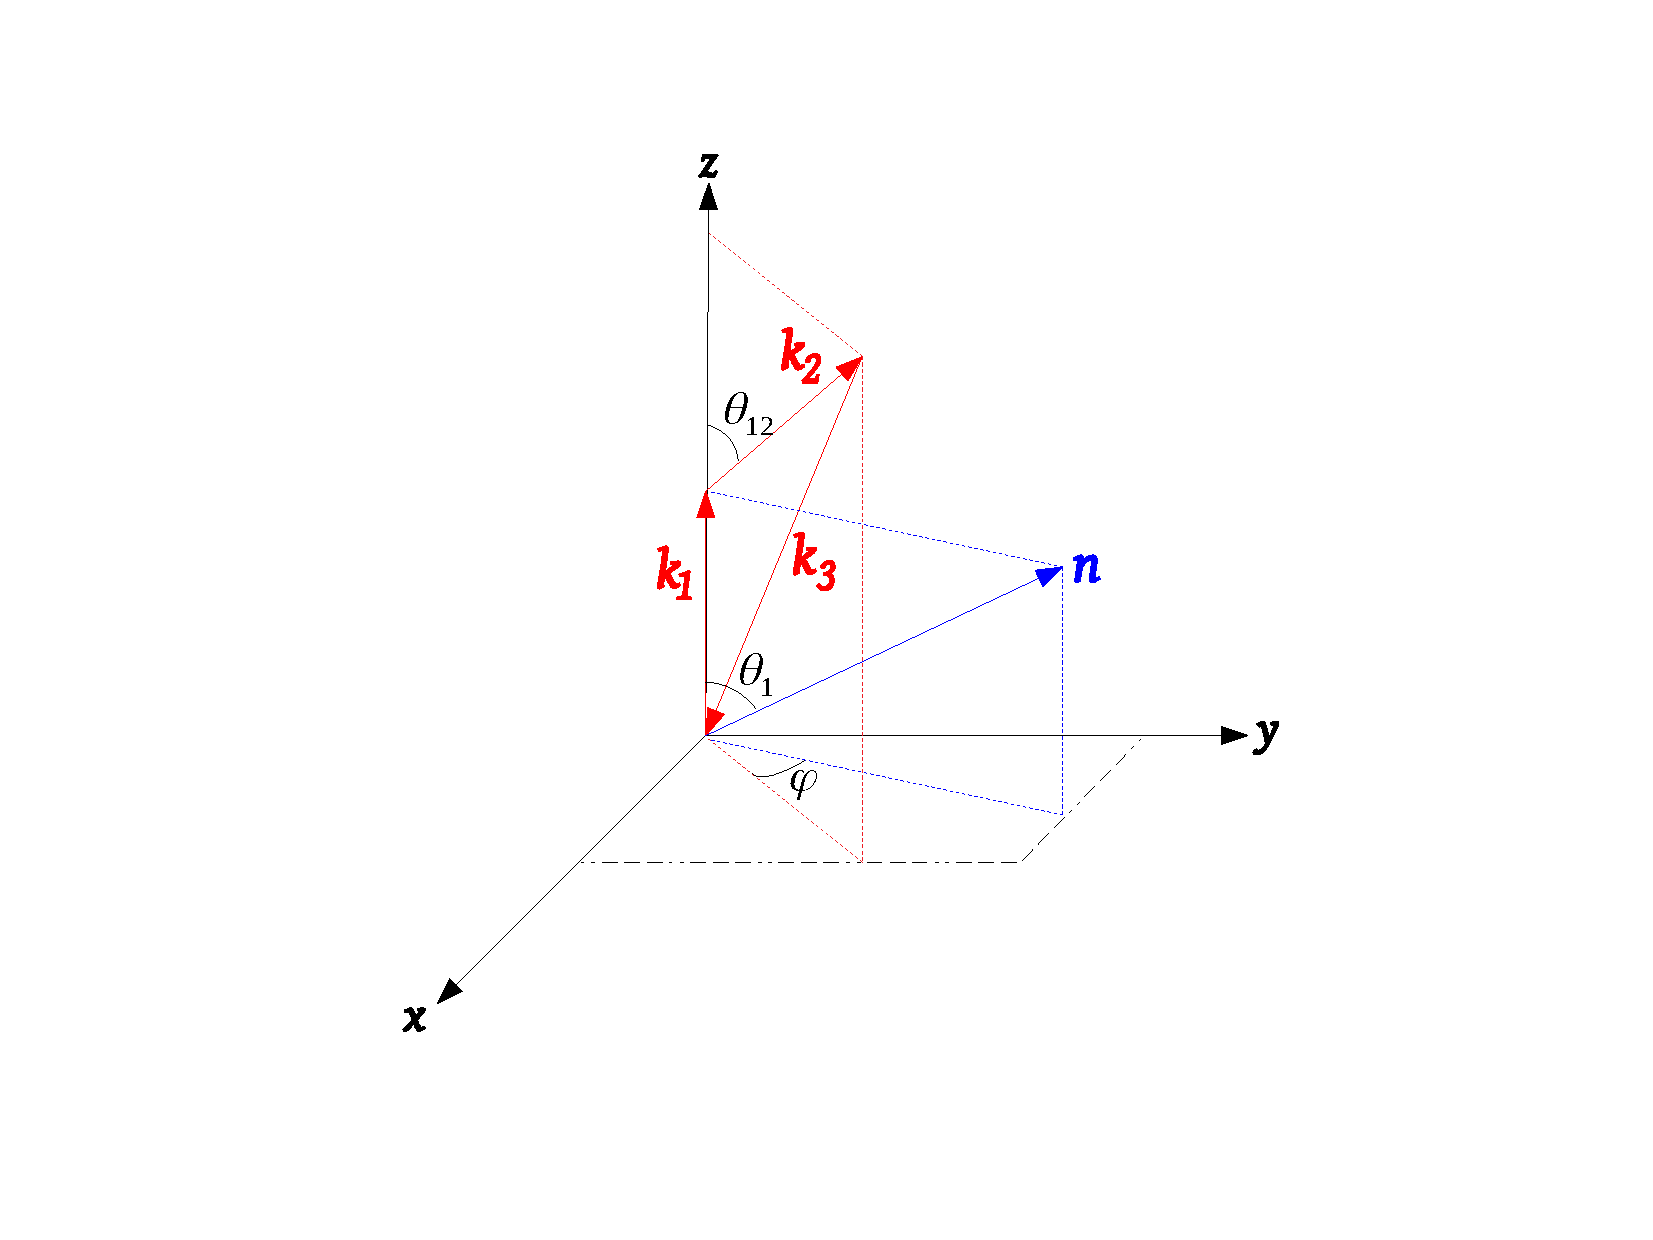
\includegraphics[width=10.0cm]{fig/geometryAngles}
\vspace*{-1cm}
\caption{Relevant vectors and angles for the Fourier bispectrum.} \label{fig0}
\end{figure}

In the standard Newtonian approximation, $B_g=B_{g{\mathrm{N}}}$, the kernels in \eqref{eq:bkern} contain the galaxy bias and the redshift-space distortions (RSD) at first and second order \cite{Bernardeau:2001qr, Karagiannis:2018jdt}:
\begin{align}
\mathcal{K}^{(1)}_{\mathrm{N}}(\bm{k}_{1}) &= b_{1}+f\mu_{1}^{2}\,,  \label{e15} \\ 
{\mathcal{K}^{(2)}_{\mathrm{N}}}(\bm{k}_{1}, \bm{k}_{2},{\bm{k}_3}) &= b_{1}F_{2}(\bm{k}_{1}, \bm{k}_{2}) + b_{2} + f\mu_{3}^{2}G_{2}(\bm{k}_{1}, \bm{k}_{2}) +{fZ_2}(\bm{k}_{1}, \bm{k}_{2})
+ b_{s^{2}}S_{2}(\bm{k}_{1}, \bm{k}_{2}) , \label{k2n}
\end{align}
where we dropped the $z$-dependence for brevity. Here $f$ is the linear matter growth rate, $b_1,b_2$ are the linear and second-order clustering biases, and $b_{s^{2}}$ is the tidal bias. The kernel  $F_2$ is for second-order density, $G_2 , \mathcal{Z}_2$ are for RSD,  and $S_2$  is the kernel for tidal bias.


The Doppler-type relativistic corrections to the Newtonian number count contrast in redshift space are  given {at first order by~\cite{Bonvin:2011bg}:}
\begin{equation}
\delta_{g\mathrm{D}} =  {A}\,\bm{v}\cdot\bm{n}\,,\label{dg1}
\end{equation}
{where $A(z)$ is given below in~\eqref{e25} and the momentum conservation equation has been used to  eliminate the gravitational redshift: $\bm{n}\cdot\bm{\nabla}\Phi\equiv \p_r \Phi = -\bm{v}'\!\cdot\bm{n}-\cH\,\bm{v}\cdot\bm{n} $.} Here $\Phi$ is the gravitational potential, $\bm{v}$ is the peculiar velocity,  $\cH$ is the comoving Hubble parameter, and $r$ is the line-of-sight comoving distance.
Note that $\bm{v}\cdot\bm{n}=\partial_r V$, where $V$ is the velocity potential ($v_i=\partial_iV$). 
At second order, and neglecting vector and tensor modes, it is shown in~\cite{Clarkson:2018dwn}  that (see also \cite{DiDio:2018zmk}) 
\begin{align}
\delta^{(2)}_{g{\mathrm{D}}}&= A\, \bm{v}^{(2)}\!\!\cdot\bm{n}+2{C}(\bm{v}\cdot\bm{n})\,\delta +2 \frac{{E}}{\cH}(\bm{v}\cdot\bm{n})\,\partial_r(\bm{v}\cdot\bm{n})
+ \frac{2}{\cH^2}\big[(\bm{v}\cdot\bm{n}) \,\partial_r^2\Phi-\Phi\, \partial_r^2 (\bm{v}\cdot\bm{n}) \big]
\nonumber\\ \label{eq:dgsecond}
& - \frac{2}{\cH}\,\partial_r (\bm{v}\cdot\bm{v}) + 2 \frac{b_1}{\cH}\,\Phi\, \partial_r\delta \,. 
\end{align}
The redshift-dependent coefficients $C,E$ are  given below  in \eqref{e26}, \eqref{e27}.


In Fourier space, 
neglecting sub-leading $ \mathcal{O}(\cH^2/k^2)$ terms, we find from \eqref{eq:bkern} that
\begin{align}
 B_{g\mathrm{D}}(\bm{k}_{1},\bm{k}_{2},\bm{k}_{3}) &=  \bigg\{\bigg[\mathcal{K}^{(1)}_{\mathrm{N}}(\bm{k}_{1})\mathcal{K}^{(1)}_{\mathrm{D}}(\bm{k}_{2}) + \mathcal{K}^{(1)}_{\mathrm{D}}(\bm{k}_{1})\mathcal{K}^{(1)}_{\mathrm{N}}(\bm{k}_{2})\bigg]\mathcal{K}^{(2)}_{\mathrm{N}}(\bm{k}_{1},\bm{k}_{2},\bm{k}_{3}) 
\nonumber \\&  \quad 
+\mathcal{K}^{(1)}_{\mathrm{N}}(\bm{k}_{1})\mathcal{K}^{(1)}_{\mathrm{N}}(\bm{k}_{2})\mathcal{K}^{(2)}_{\mathrm{D}}(\bm{k}_{1},\bm{k}_{2},\bm{k}_{3})\bigg\}P(k_{1})P(k_{2})+\text{2 cp}. \label{e21}
\end{align}
The relativistic kernels follow from \eqref{dg1} and \eqref{eq:dgsecond}; they are given in \cite{Clarkson:2018dwn} as
\begin{align}
\mathcal{K}^{(1)}_{\mathrm{D}}(\bm{k}_{1}) &= \mathrm{i}\,\cH f A\,\frac{\mu_{1}}{k_{1}}\,, \label{e23} \\
\mathcal{K}^{(2)}_{\mathrm{D}}(\bm{k}_{1},\bm{k}_{2},\bm{k}_{3}) &= \mathrm{i}\,\cH f \bigg[
A\,\frac{\mu_{3}}{k_{3}}G_{2}(\bm{k}_{1},\bm{k}_{2})
+C\left(\frac{\mu_{1}}{k_{1}} + \frac{\mu_{2}}{k_{2}}\right)
 +\left(\frac{3}{2}\Omega_{m}-fE\right)\mu_{1}\mu_{2}\left(\frac{\mu_{1}}{k_{2}}+\frac{\mu_{2}}{k_{1}}\right)
\nonumber \\
&\hspace*{-1.5cm}  
{} -\frac{3}{2}\Omega_{m}\left(\mu_{1}^{3}\frac{k_{1}}{k_{2}^{2}} + \mu_{2}^{3}\frac{k_{2}}{k_{1}^{2}}\right)
+2f\,  {\hat{\bm{k}}_{1} \cdot \hat{\bm{k}}_2}\left(\frac{\mu_{1}}{k_{1}} + \frac{\mu_{2}}{k_{2}}\right) 
 -\frac{3\Omega_{m}b_1}{2f}\left(\mu_{1}\frac{k_{1}}{k_{2}^{2}} + \mu_{2}\frac{k_{2}}{k_{1}^{2}}\right)\!  \bigg]\! .~~~ \label{e24}
\end{align}
It is clear from \eqref{e21}--\eqref{e24} and from the general expressions given in {\cite{Umeh:2016nuh,Jolicoeur:2017nyt}}, that Doppler-type relativistic effects generate an imaginary correction to the Newtonian bispectrum: 
\begin{equation}
{{\mathrm{Re}}\, B_g =B_{g\mathrm{N}} + \mathcal{O}(\cH^2/k^2)\,,~~ {\i}\, {\mathrm{Im}}\, B_g = B_{g\mathrm{D}}+ \mathcal{O}(\cH^3/k^3)}\,. \label{bgnd}
\end{equation}

The  coefficients in~\eqref{e23} and~\eqref{e24} are~\cite{Clarkson:2018dwn}
\begin{align}
A &= b_{e} - 2\mathcal{Q} + \frac{2(\mathcal{Q}-1)}{{r} \cH}
 - \frac{\cH'}{\cH^{2}} \label{e25} \,, \\
C &= b_{1}\big(A+f) + \frac{b_1'}{\cH} + 2\bigg(1-\frac{1}{{r} \cH}\bigg){\frac{\partial b_1}{\partial \ln{L}}\bigg|_{\mathrm{c}}} \label{e26}\,, \\
E &= 4-2A-\frac{3}{2}\Omega_{m} \label{e27} \,,
\end{align}
where a prime is a conformal time derivative, $\Omega_m=\Omega_{m0}(1+z)H_0^2/\cH^2$,  $L$ is the  luminosity, and $\,|_{\mathrm{c}}$ denotes evaluation at the flux cut. 

In addition to the clustering bias  $b_1$, the relativistic bispectrum is sensitive to  the evolution bias and magnification bias, which  are defined as \cite{Alonso:2015uua}
\begin{equation} \label{bq}
b_e=  - \frac{\partial \ln n_g}{\partial\ln (1+z)}\,,~~~{ {\cal Q} =- \frac{\partial \ln n_g}{\partial\ln L}\bigg|_{\mathrm{c}}}\,.
\end{equation}
Here and below,  $n_{g}$ is the {\em comoving} galaxy number density.  (Note that the alternative magnification bias parameter  $s=2{\cal Q}/5$ is often used.)

{It is interesting to note that the magnification bias ${\cal Q}$ enters the relativistic bispectrum, even though we have not  included the effect of the integrated lensing magnification $\kappa$. The reason for this apparent inconsistency is that there is a (non-integrated) Doppler correction to $\kappa$ at leading order \cite{Bonvin:2008ni,Bolejko:2012uj}.} 


\section{Signal-to-Noise}

The signal-to-noise ratio (SNR) for the bispectrum at some redshift $z$ is in the Gaussian approximation of uncorrelated triangles given by~\citep{Scoccimarro:2003wn}, 
\begin{equation}
\left[\frac{S}{N}(z)\right]^{2} = 
\sum_{k_a,\,\mu_{1},\,\varphi}\,\frac{1}{{\mathrm{Var}} [{B_{g}}(z, k_a,\mu_{1},\varphi)]}
\,B_{g}(z, k_{a},  \mu_{1},\varphi)\,B^*_{g}(z, k_a, \mu_{1},\varphi)\,,\label{eq:snrdef} 
\end{equation} 
where we have introduced the complex conjugate $B^*_g$ as the galaxy bispectrum has an imaginary correction. Here ${\mathrm{Var}} [{B_{g}}]$ is the variance of the bispectrum estimator \citep{Chan:2016ehg},
\begin{equation} \label{hatb}
\hat{B}_g(z,\bm{k}_a) = \frac{k_{\mathrm{f}}^3}{V_{123}}\int_{\bm{k}_a}\ud^3\bm{q}_1\, \ud^3\bm{q}_2 \,\ud^3\bm{q}_3\,\delta^{{\mathrm{Dirac}}}(\bm{q}_1+\bm{q}_2+\bm{q}_3)\, \delta_g(z,\bm{q}_1) \delta_g(z,\bm{q}_2) \delta_g(z,\bm{q}_3) \,,
\end{equation}
where integration is over the shells $k_a-\Delta k/2\leq q_a \leq k_a+\Delta k/2$ and  the shell volume is
$V_{123}=\int_{\bm{k}_a}\ud^3\bm{q}_1\, \ud^3\bm{q}_2 \,\ud^3\bm{q}_3\,\delta^{{\mathrm{Dirac}}}(\bm{q}_1+\bm{q}_2+\bm{q}_3)$.


In the Newtonian approximation, the Gaussian variance can be given as \citep{Scoccimarro:2003wn, Karagiannis:2018jdt},
\begin{equation}
\mathrm{Var} [{B_{g}}(z, k_a,\mu_{1},\varphi)] = s_B\, \frac{\pi k_{\mathrm{f}}(z)^3}{k_1k_2k_3 (\Delta k)^3}\,\frac{N_{\mu_1}N_\varphi}{\Delta \mu_1 \Delta \varphi} \, \tilde{P}_{g{\mathrm{N}}}(z,k_{1},\mu_{1}) \tilde{P}_{g{\mathrm{N}}}(z,k_{2},\mu_{2})\tilde{P}_{g{\mathrm{N}}}(z,k_{3},\mu_{3})\,,
\label{eq:gaussvar} 
\end{equation}
where,
\begin{equation}
\tilde{P}_{g{\mathrm{N}}}(z, k_{a}, \mu_{a}) = P_{g{\mathrm{N}}}(z, k_{a}, \mu_{a}) + \frac{1}{n_g(z)}\,, \label{eq:Pgdef} 
\end{equation}
and ${P}_{g{\mathrm{N}}}=(b_1+f\mu_a^2)^2P$ is the linear galaxy power spectrum.
In \eqref{eq:gaussvar}, $s_{B}$ is 6, 2, 1 respectively for equilateral, isosceles and non-isosceles triangles, and $N_{\mu_1},N_\varphi$ are the ranges for $\mu_1,  \varphi $ (which are sometimes reduced from their full values of 2 and $2\pi$ using symmetry arguments).
The fundamental mode is determined by the comoving survey volume of the redshift bin centred at $z$, i.e.,
\begin{equation}\label{eq:kfundamental}
    k_{\mathrm{f}}(z) = {2\pi}{V(z)^{-1/3}}\,,
\end{equation}
where $V(z)=4\pi  f_{\mathrm{sky}}[r(z+\Delta z/2)^3 - r(z-\Delta z/2)^3]$.

For a survey with redshift bin centres ranging from $z_{\mathrm{min}}$ to $z_{\mathrm{max}}$,  the cumulative SNR  is
\begin{equation} \label{csnr}
\frac{S}{N}\big(\leq z\big) = \left\{\sum_{z'=z_{\mathrm{min}}}^z \left[\frac{S}{N}(z')\right]^{2} \right\}^{1/2}\,,
\end{equation}
and then the total SNR is $S/N(\leq z_{\mathrm{max}})$.
%

\subsection{Relativistic contributions to the variance}
%
%
For the full bispectrum, including the relativistic part,~\eqref{hatb} leads to a variance of the form 
\begin{equation} \label{varb}
\mathrm{Var} [{B_{g}}(z,\bm{k}_a)] \propto \tilde{P}_{g}(z,k_{1},\mu_{1}) \tilde{P}_{g}(z,k_{2},\mu_{2})\tilde{P}_{g}(z,k_{3},\mu_{3}) \,.
\end{equation}
In the Newtonian approximation, this gives~\eqref{eq:gaussvar}. By~\eqref{e23}, the galaxy number density contrast has an imaginary relativistic correction, $\delta_g=\delta_{g\mathrm{N}} + \delta_{g\mathrm{D}}$. However, since $P_g \sim\langle \delta_g(\bm{k}) \delta_g(\bm{-k})\rangle =\langle |\delta_g(\bm{k})|^2\rangle$, the galaxy power spectrum is given by~\cite{McDonald:2009dh,Abramo:2017xnp,Clarkson:2018dwn},
\begin{equation} \label{pgnd}
P_g = P_{g\mathrm{N}} + P_{g \mathrm{D}} =  P_{g \mathrm{N}} + \ord(\cH^2/k^2)\,.
\end{equation}
It follows from~\eqref{varb} and~\eqref{pgnd} that at leading order, the relativistic contribution to the variance can be neglected,
\begin{equation}
\mathrm{Var} [{B_{g}}] = \mathrm{Var} [B_{g\mathrm{N}}] + \ord(\cH^2/k^2)\,.
\end{equation}
Therefore the SNR for the Newtonian and relativistic parts of the bispectrum are,
\begin{align}
\left(\frac{S}{N}\right)^2_\mathrm{N} &= 
\sum_{k_a,\,\mu_{1},\,\varphi}\, \frac{B_{g \mathrm{N}}\,B_{g\mathrm{N}}}{\mathrm{Var} [B_{g \mathrm{N}}] }\,,\label{e3a}\\
\left(\frac{S}{N}\right)^{2}_\mathrm{D} &= 
\sum_{k_a,\,\mu_{1},\,\varphi} \, \frac{ B_{g \mathrm{D}} \, B^*_{g \mathrm{D}}  }{ \mathrm{Var} [B_{g{\mathrm{N}}}]}\,.\label{e3b}  
\end{align}
%
%
\subsection{Nonlinear effects}
%
%
In order to avoid nonlinear effects of matter clustering, the maximum $k$ is chosen as a scale where perturbation theory for the matter density contrast begins to break down. It is known that the matter bispectrum is more sensitive to nonlinearity than the matter power spectrum: at $z\sim 0$ nonlinearity sets in at $k\sim 0.1h/\,$Mpc for the matter bispectrum, as opposed to $k\sim 0.2h/\,$Mpc for the matter power spectrum. To account for the growth of $k_{\mathrm{max}}$ with redshift, we use the redshift-dependence proposed in~\cite{Smith:2002dz} for the power spectrum, but with half the amplitude at $z=0$,
\begin{equation}\label{kmax}
k_\mathrm{max}(z) = {0.1h}\left(1+z\right)^{2/(2+n_{s})}\,.
\end{equation}

The cut-off $k\leq k_\mathrm{max}(z)$ avoids a breakdown of perturbative accuracy in the matter correlations, but nonlinearities in the galaxy correlations due to RSD can affect longer wavelength modes. The effect of RSD on these scales is to damp the power -- the `FoG' effect. In order to take account of this, we follow~\cite{Karagiannis:2018jdt,Yankelevich:2018uaz} and use the simple model of FoG damping,
\begin{align}
&P_g \to  D_P\, P_g\,,\quad~ D_{P}(z, \bm{k}) = \exp\left\{-\frac{1}{2}{\left[k\mu\,\sigma(z)\right]^{2}}\right\}\,, \\
&B_g \to  D_B\, B_g\,,  \quad D_{B}(z, \ka,\kb,\kc) = \exp\left\{-\frac{1}{2}{\left[k_{1}^{2}\mu_{1}^{2}+k_{2}^{2}\mu_{2}^{2}+k_{3}^{2}\mu_{3}^{2}\right]\sigma(z)^{2}}\right\}\,, \label{e13}
\end{align}
where $\sigma$ is the linear velocity dispersion.

On sufficiently large scales the non-Gaussian contribution to the bispectrum covariance can be  approximated by including corrections to the power spectra appearing in the bispectrum variance~\eqref{e4}. This is shown by~\cite{Chan:2016ehg} (see also~\cite{Karagiannis:2018jdt}), using the approximation,
\begin{align}
\mathrm{Var} [B_{g}] &\to \mathrm{Var} [B_{g}]+ \delta \mathrm{Var} [B_{g}] \,, \\
\delta \mathrm{Var} [B_{g}] &= \frac{s_B\pi k_\mathrm{f}^3 N_{\mu_1} N_\varphi}{k_1 k_2 k_3 (\Delta k)^3\Delta \mu_1 \Delta \varphi}\, \left\{ \tilde{P}_{g \mathrm{N}}(1) \tilde{P}_{g \mathrm{N}}(2) \left[ \tilde{P}^\mathrm{NL}_{g \mathrm{N}}(3) - \tilde{P}_{g\mathrm{N}}(3) \right] + 2 \, \mbox{cp} \right\}\,.
\label{e4x}
\end{align}
Here $\tilde{P}_{g \mathrm{N}}(a) \equiv \tilde{P}_{g \mathrm{N}}(z,k_a,\mu_a)$ and $\tilde{P}^{\mathrm{NL}}_{g{\mathrm{N}}}(a) = (b + f \mu_a^2)^2 P^\mathrm{NL} + n_g^{-1}$, where $P^{\mathrm{NL}}$ is the nonlinear matter power spectrum, computed with a modified Halofit emulator.
%
%
\subsection{Summations over triangles}

The counting of triangles $\ka + \kb + \kc = \bm{0}$ that contribute to the signal-to-noise involves a sum in $k_a$-space and a sum over orientations.

The triangle sides are chosen so that $k_1\geq k_2 \geq k_3$, and must satisfy $k_1-k_2-k_3\leq 0$.
For the summation in $k_a$ we choose the minimum and the step-length as
\begin{equation}
k_\mathrm{min}(z) = k_\mathrm{f}(z)~~\mbox{and}~~ \Delta k(z)=k_{\mathrm{f}}(z) \,,
\end{equation}
as in~\cite{Karagiannis:2018jdt,Yankelevich:2018uaz}. 
Then the $k_a$ sum is defined as~\cite{Liguori:2010hx,Oddo:2019run}
\begin{equation}
\sum_{k_a} = \sum_{k_{1} = k_\mathrm{min}}^{k_\mathrm{max}} \, \sum_{k_{2}=k_{\mathrm{min}}}^{k_{1}}\,\sum_{k_{3}=k_{\mathrm{min}}}^{k_{2}}
\,.\label{e8}
\end{equation} 

The coordinates $(\mu_1=\cos\theta_{1},\varphi)$ describe all possible orientations of the triangle. 
We follow~\cite{Karagiannis:2018jdt} and choose the ranges $N_{\mu_1}=2, N_{\varphi}=2\pi$.
For a given $\mu_{1}$, a complete rotation in $\varphi$ about $\bm{k}_1$ double counts the  triangle falling onto the fixed $(\bm{n},\bm{k}_1)$-plane at $\varphi=0$ and $\varphi=2\pi$ (see~\ref{fig0}). Similarly, for a given $\varphi$,  the end-points $\theta_1=0$ and $\theta_1=\pi$  correspond to equivalent triangles, with $\bm{k}_a \to - \bm{k}_a$.
This double-counting can be avoided by imposing suitable upper limits:
$-1\leq \mu_1 <1$ and $0\leq \varphi < 2\pi$.
The signal to noise is quite sensitive to the step-lengths $\Delta \mu_{1}, \Delta\varphi$. Figure~\ref{fig4x} shows the effect on the relativistic total SNR of changing the number of orientation bins, $n_{\mu_1}=N_{\mu_1}/\Delta{\mu_1}=2 /\Delta{\mu_1}$  and $n_\varphi=N_\varphi/\Delta\varphi =2\pi/\Delta\varphi$. It is apparent that reducing the number of bins increases the cumulative SNR. The cumulative SNR converges towards a minimum for $n_{\mu_{1}}\,, n_{\varphi} > 40$.
\begin{figure}[ht]
\centering
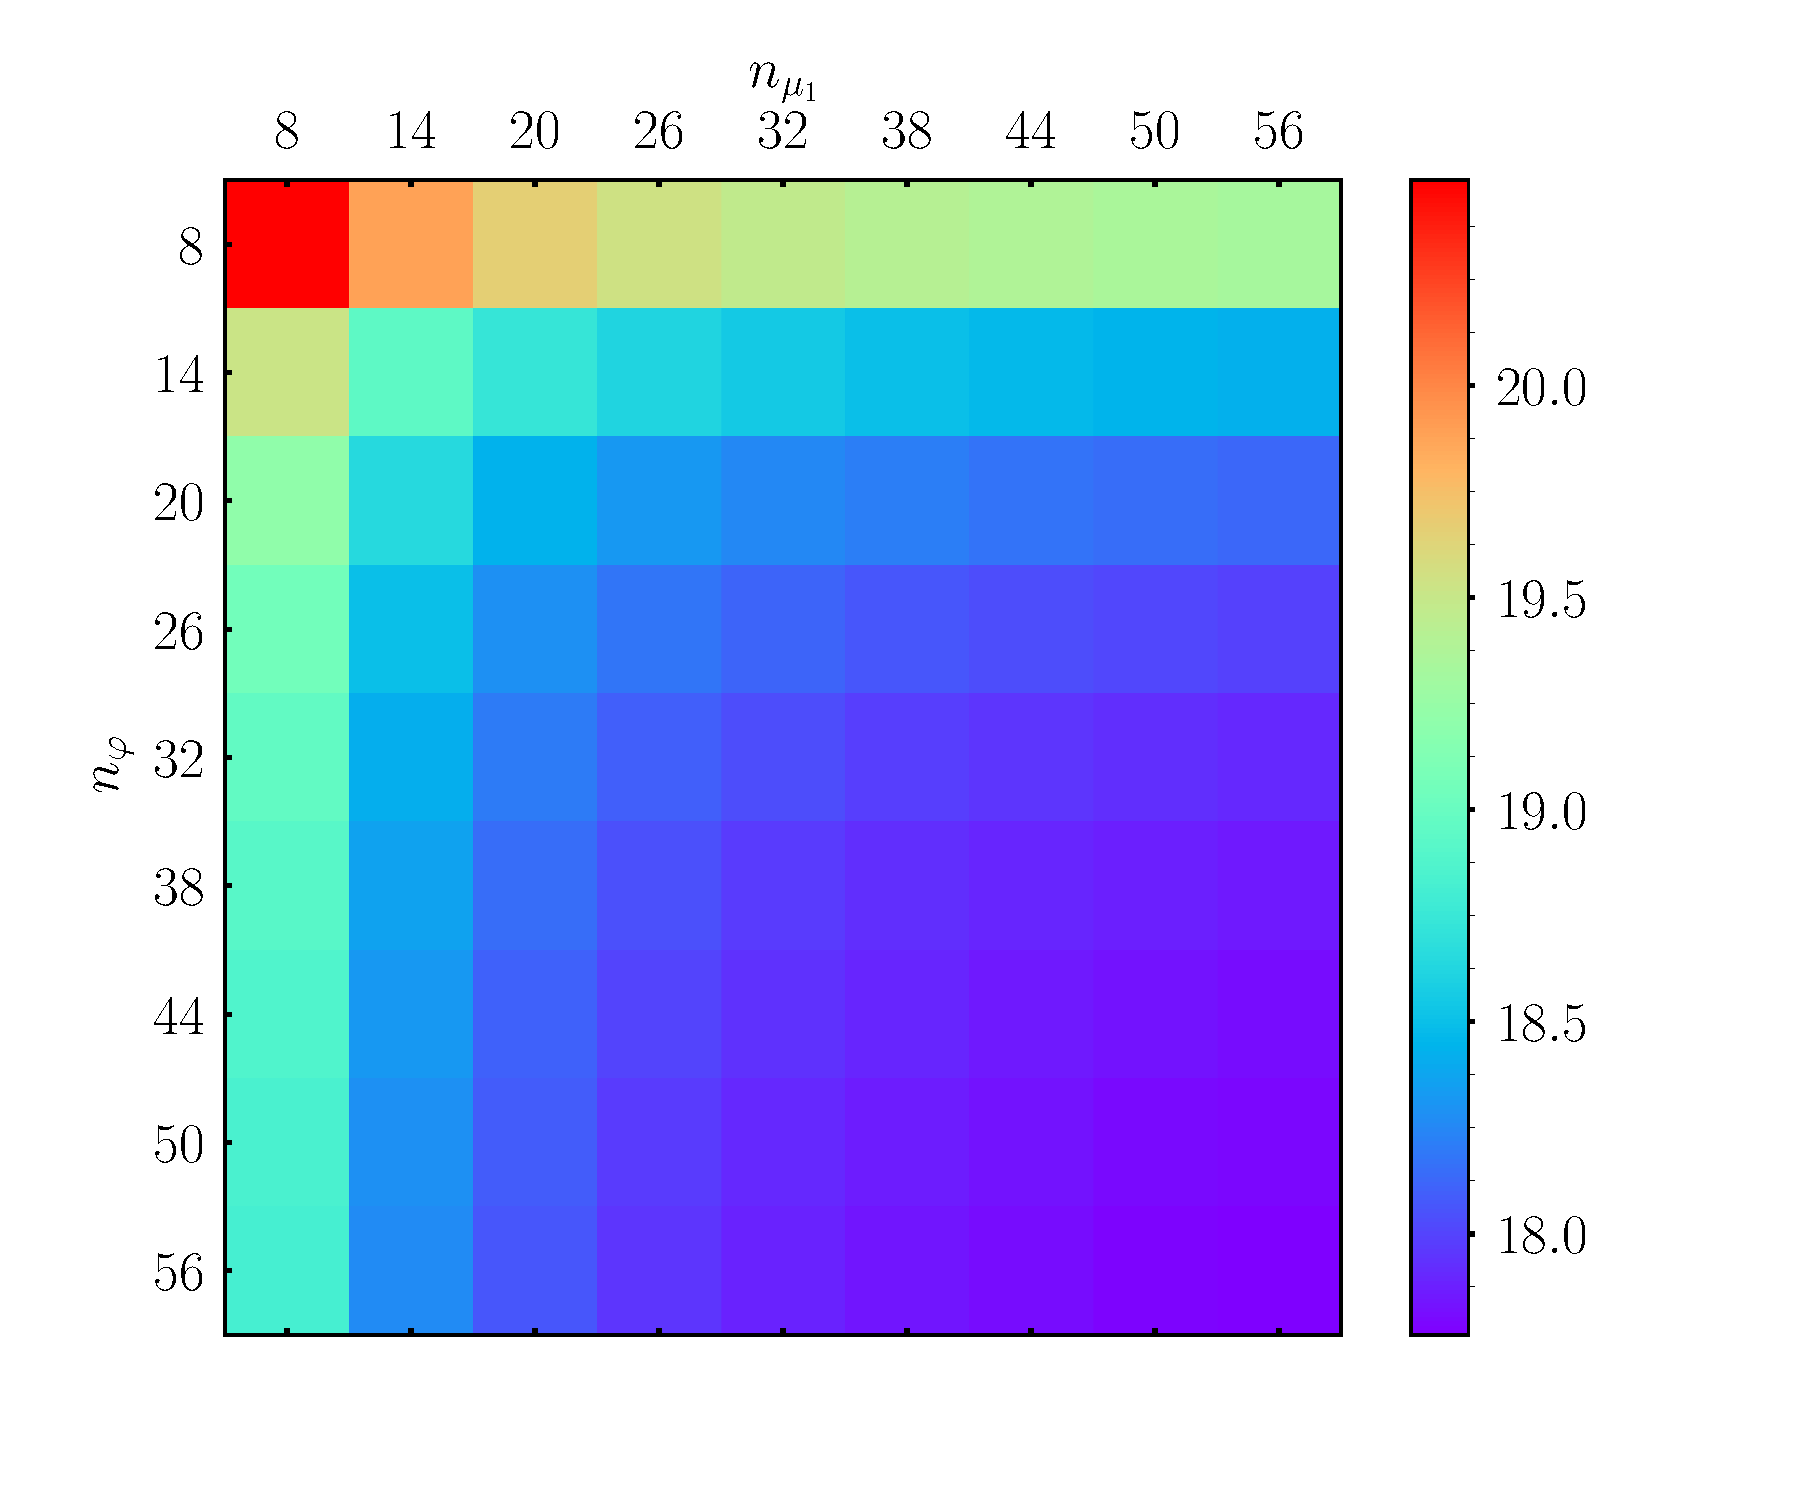
\includegraphics[width=8.0cm]{fig/colournmu1nphi_Doppler-eps-converted-to} 
\caption{Effect on 
{total} relativistic SNR of changing number of  $\varphi$ and $\mu_1$ bins. 
} \label{fig4x}
\end{figure} 
%
Following this, we find that a suitable choice for convergence is
\begin{equation}\label{ori}
\Delta \mu_{1}=0.04\,,~~ \Delta\varphi= \pi/25 \,,
\end{equation}
or $n_{\mu_{1}}= n_{\varphi}=50$.

\section{Next-generation galaxy surveys}
%
\begin{figure}[ht]
\centering
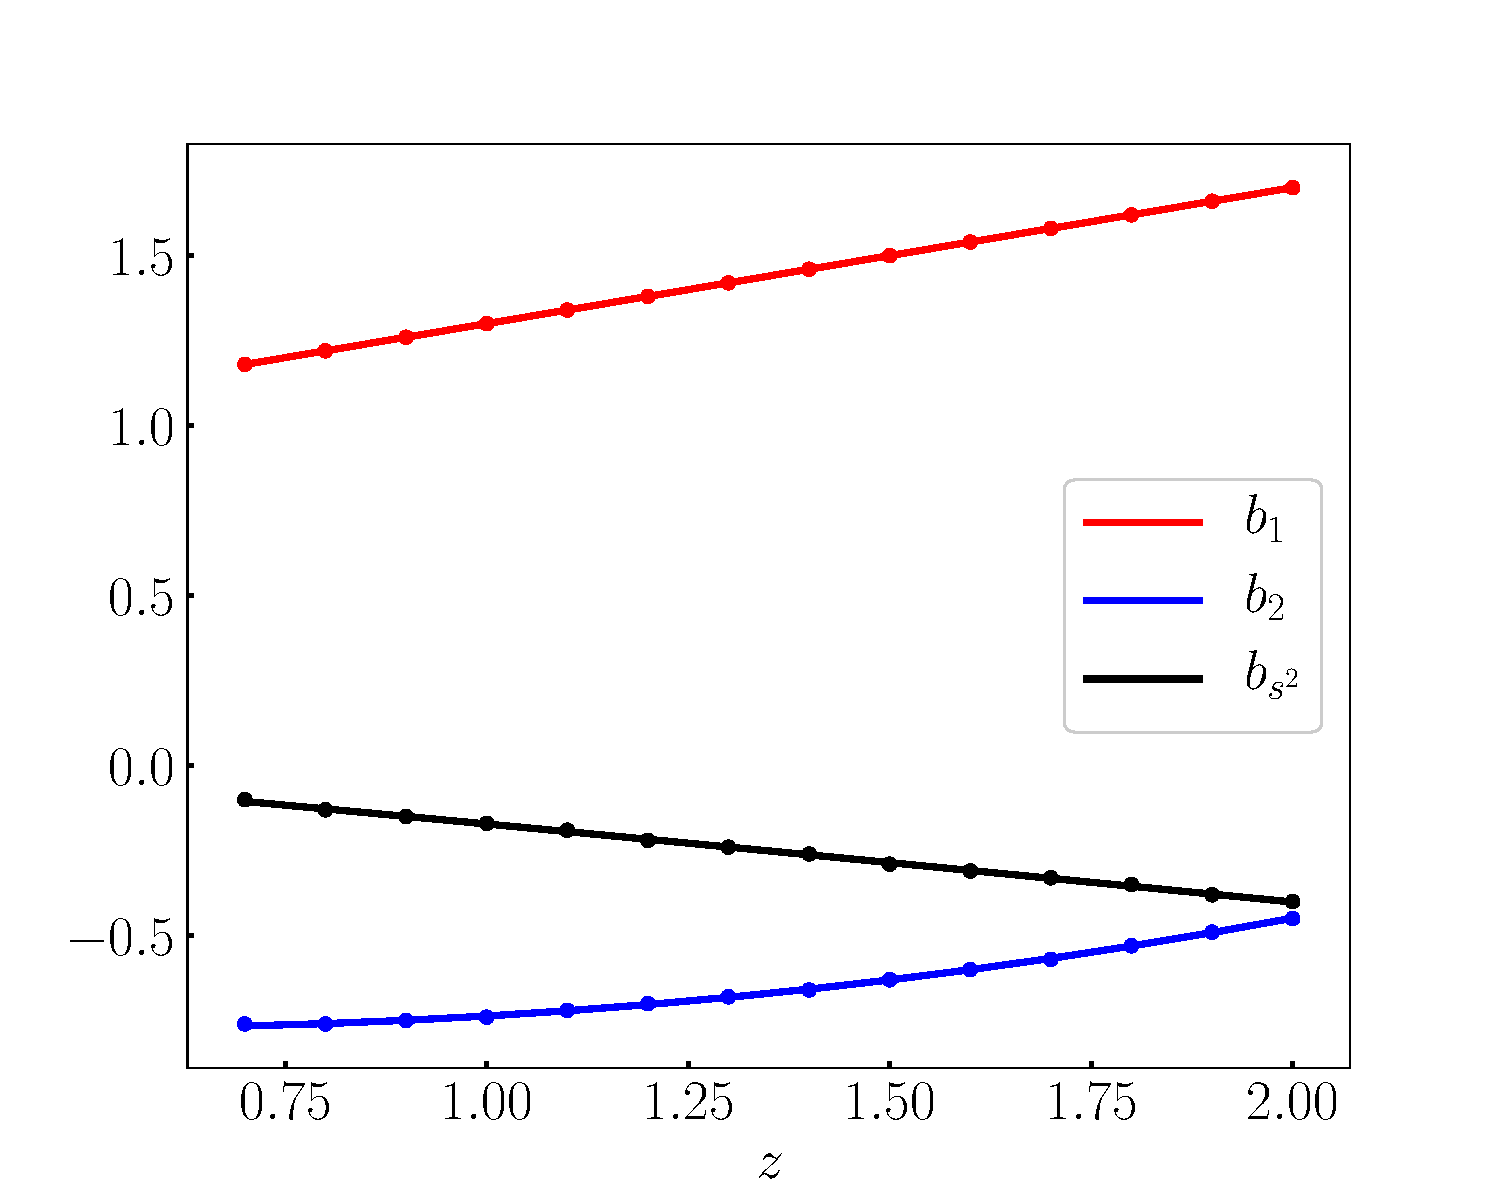
\includegraphics[width=5.cm]{fig/b-eps-converted-to}
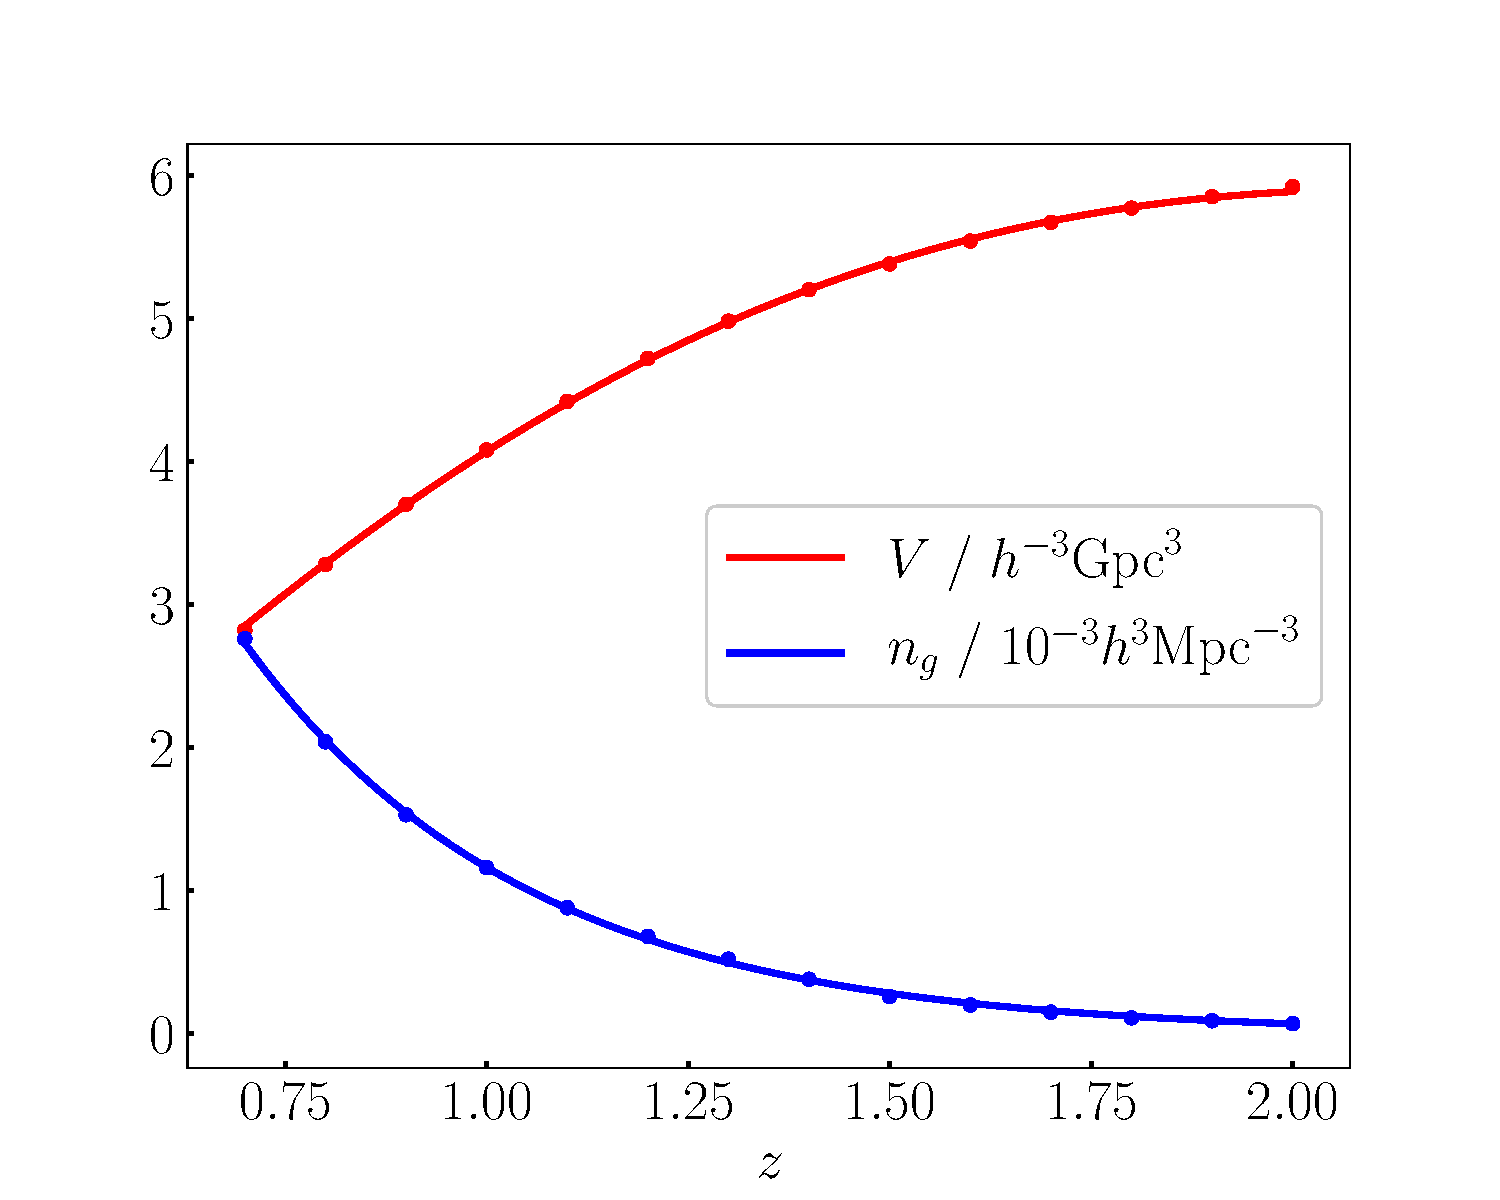
\includegraphics[width=5.cm]{fig/V_n-eps-converted-to} 
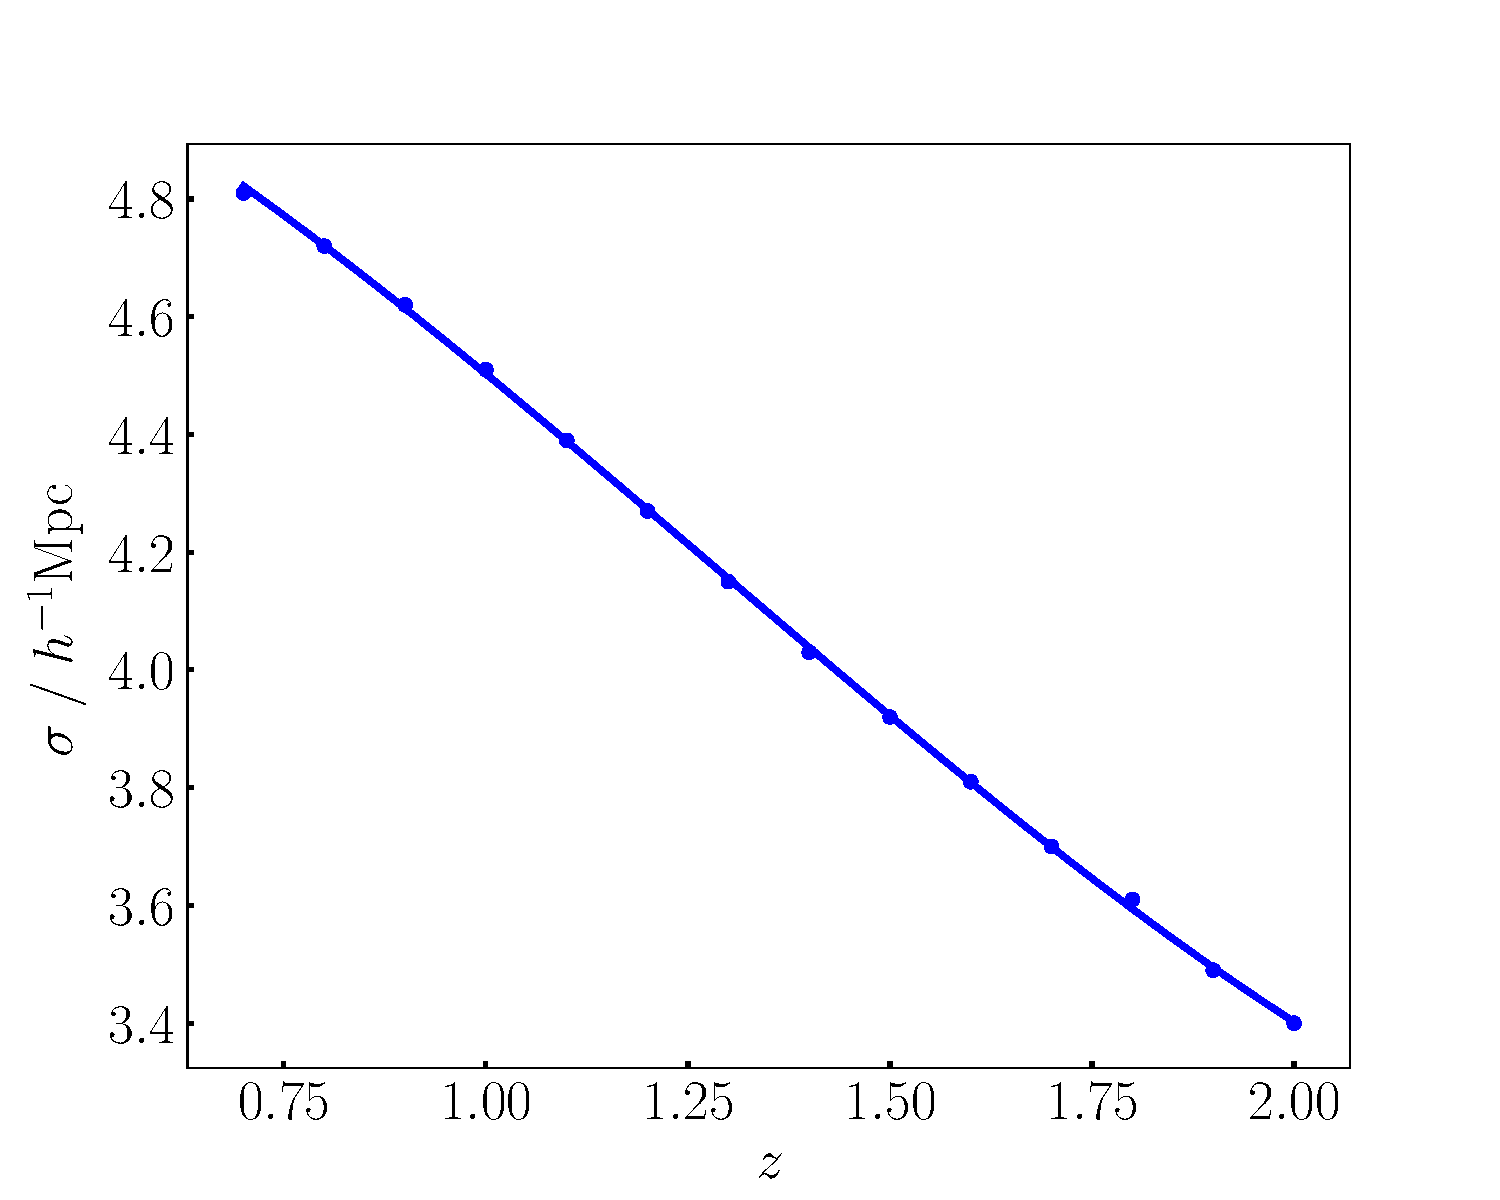
\includegraphics[width=5.cm]{fig/sigma-eps-converted-to}
\caption{Clustering bias parameters ({\em left}), comoving volume and number density ({\em middle}) and RSD damping parameter ({\em right}). Points are the data from Table 1 in~\cite{Yankelevich:2018uaz}.}
\label{fig1}
\end{figure}
%
We consider a Stage IV $H\alpha$ spectroscopic survey, with clustering bias, comoving volume, comoving number density and RSD damping parameter given by Table 1 in~\cite{Yankelevich:2018uaz}, over the redshift range $0.65\leq z\leq 2.05$, with $\Delta z=0.1$ bins. 
Fitting formulas for these quantities are, 
\begin{align}
b_1(z) &= 0.9+0.4 z\,, \quad b_2(z) = -0.741 - 0.125\,z + 0.123\,z^{2} + 0.00637\,z^{3}\,, \label{e9}  \\
 b_{s^2}(z) &= 0.0409 - 0.199\,z - 0.0166\,z^{2} + 0.00268\,z^{3} \,, \label{e11} \\
 V(z) &= 8.85\, z^{1.65}\exp\big({-0.777\,z}\big)~ h^{-3}\,\mathrm{Gpc}^{3}\,, \label{e11_1} \\
n_{g}(z) &= 0.0193\, z^{-0.0282}\exp\big({-2.81\,z}\big) ~h^{3}\,\mathrm{Mpc}^{-3}\,,
 \label{e11_2}\\
\sigma(z)& = \big(5.29 - 0.249\,z - 0.720\,z^{2} + 0.187\,z^{3}\big)~h^{-1}\,\mathrm{Mpc}\,. \label{e14a}
\end{align}
Figure~\ref{fig1} shows the values given in~\cite{Yankelevich:2018uaz} together with the fitting curves. For the cosmological parameters, we use Planck 2018~\cite{Aghanim:2018eyx},
$h = 0.6766, \Omega_{m0} = 0.3111,
\Omega_{b0}h^{2}= 0.02242,
\Omega_{c0} h^{2} = 0.11933,
n_s = 0.9665,
\sigma_8 = 0.8102, \gamma=0.545,
\Omega_{K0} = 0= \Omega_{\nu 0}$.

We checked that the SNR for the Newtonian bispectrum is consistent with Fig.~4 of~\cite{Yankelevich:2018uaz}, when we use their redshift-independent $k_{\mathrm{max}} = 0.15h\;\mathrm{Mpc}^{-1}$, and when we remove the flattened triangle shapes that are excluded by~\cite{Yankelevich:2018uaz}. When we include the flattened shapes, we checked that we recover the total number of triangles given in Table~1 of~\cite{Oddo:2019run}.
%
%
\subsection{Evolution bias and magnification bias}

The relativistic bispectrum depends  also on $b_e$  and ${\cal Q}$, as shown in \eqref{e24}--\eqref{e27}.
These parameters do {\em not} appear in the Newtonian approximation, but they are crucial for the relativistic correction, and we need to evaluate them in a physically consistent way. We compute these parameters from the same luminosity function that is  used to generate the number density shown in Fig. \ref{fig1}, i.e., Model~1 in \cite{Pozzetti:2016cch}:
\begin{equation}
\Phi( z,y) = \Phi_{*}(z) y^\alpha\,{\mathrm{e}}^{-y}\,, \quad y\equiv \frac{L}{L_{*}}\,.
\label{e12_3}
\end{equation}
We have written $\Phi$ in terms of the redshift $z$ and the normalised dimensionless luminosity $y$, where $L_*=L_{*0}(1+z)^\delta$ and $L_{*0}$ is a characteristic luminosity.   Here
 $\alpha$ is the faint-end slope, 
and $\Phi_{*}$ is a characteristic comoving density of $H\alpha$ emitters, modelled as 
\begin{align}
\frac{\Phi_{*}}{\Phi_{*0}}= \,
\begin{cases} (1+z)^{\epsilon} &   z \leq z_{\mathrm{b}}\,,\\
(1+z_{\mathrm{b}})^{2\epsilon}(1+z)^{-\epsilon} & z > z_{\mathrm{b}} \,.
\end{cases}
\end{align}
The best-fit parameters for Model 1 are given by \cite{Pozzetti:2016cch} as 
\begin{equation} \label{eucp}
\alpha=-1.35\,, ~~\delta=2\,,~~ L_{*0}=10^{41.5}\,\mathrm{erg\,s}^{-1}\,,~~\Phi_{*0}=10^{-2.8}\,\mathrm{Mpc}^{-3}\,,~~\epsilon=1\,,~~z_{\mathrm{b}}=1.3  \,. 
\end{equation}
The flux cut  
 $F_{\mathrm{c}}$
 translates to a luminosity cut:
 \begin{equation} \label{lc}
 L_{\mathrm{c}}(z)=4\pi F_{\mathrm{c}} \,d_L(z)^2\,,\quad F_{\mathrm{c}} =3\times10^{-16}\,\mathrm{erg\,cm^{-2}\,s^{-1}} \,,
 \end{equation}
where $d_L$ is the background luminosity distance and the choice of $F_{\mathrm{c}}$ follows \cite{Yankelevich:2018uaz}. 
\begin{figure}[ht]
\centering
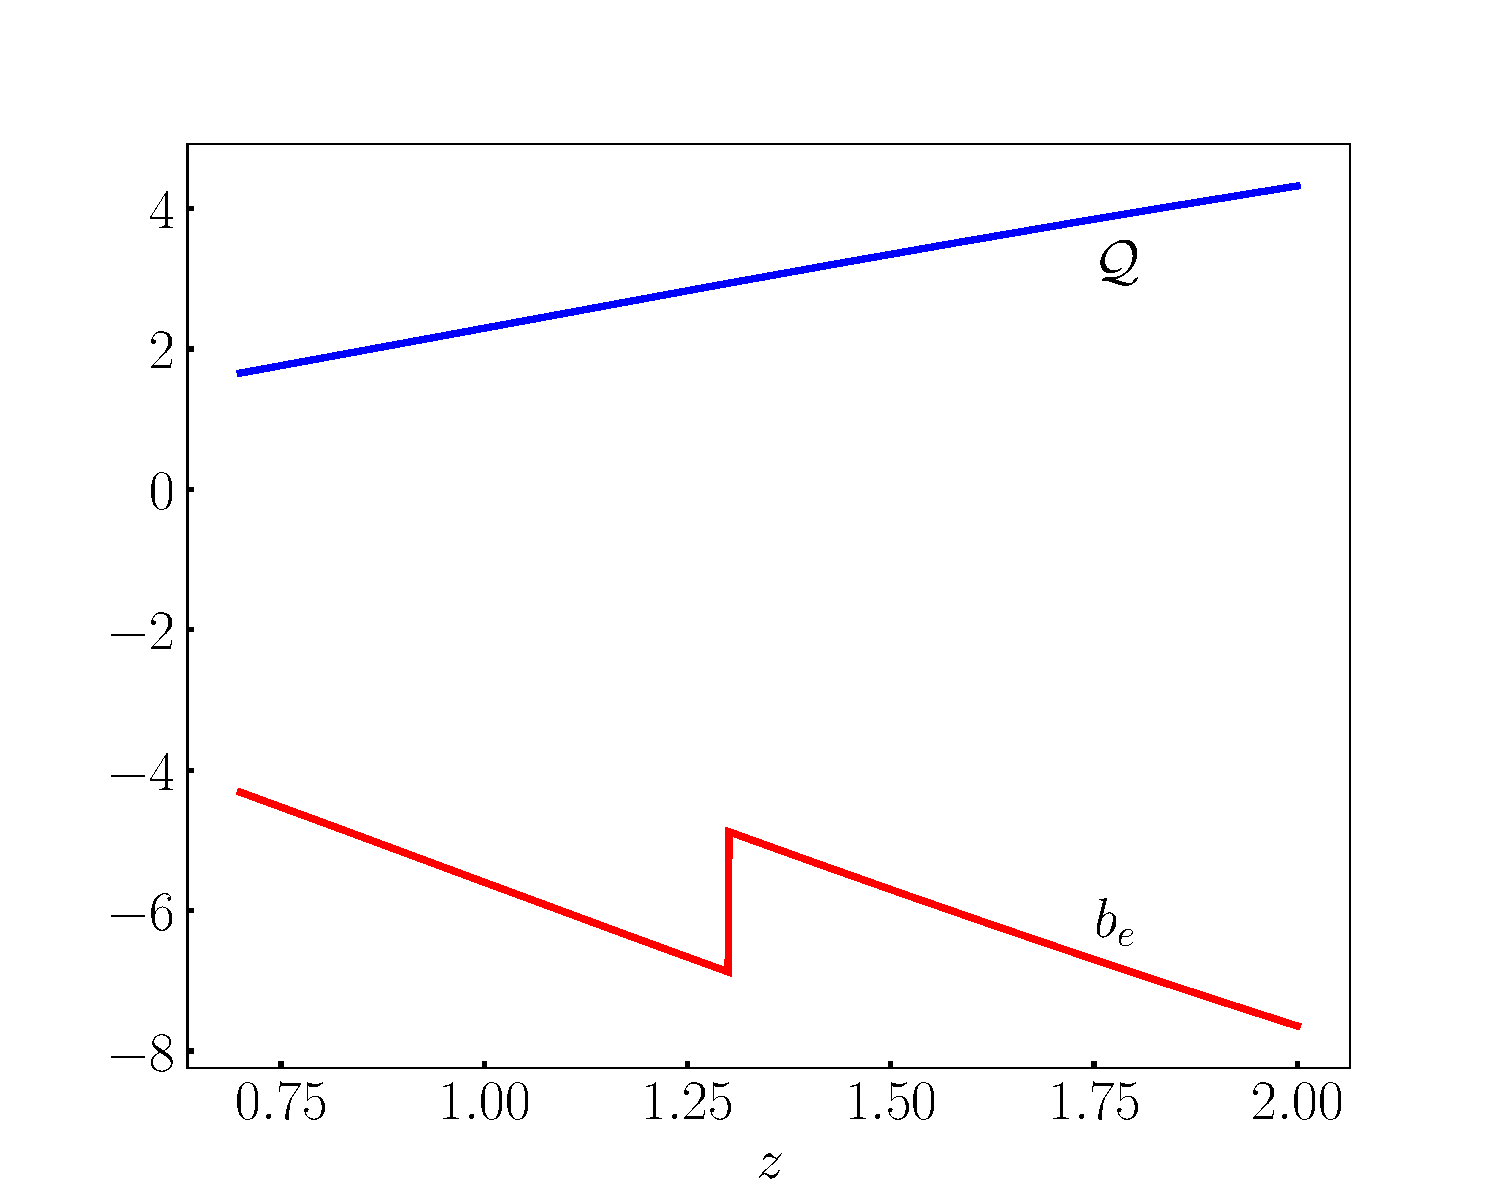
\includegraphics[width=8.0cm]{fig/beQ-eps-converted-to}
\caption{Magnification and evolution bias \eqref{q}, \eqref{be}.} 
\label{fig2}
\end{figure}

In order to compute $b_{e}$ and $\Q$, we require the comoving number density
\begin{equation} \label{ng}
n_g(z)=\int_{y_c(z)}^\infty {\ud  y}\, \Phi(z,y) = \Phi_*(z) \, \Gamma({\alpha+1}, y_c(z)) \,,
\end{equation}
where $\Gamma$ is the upper incomplete Gamma function and
\begin{equation}  \label{ycz}
y_c(z) = \frac{4\pi F_{\mathrm{c}}}{L_{*0}}\, {r}(z)^2  = \left[ \frac{{r}(z)}{2.97\,h\times 10^3~ ({\mathrm{Mpc}}/h)}\right]^2 \,.
\end{equation}
Using \eqref{ycz} and \eqref{e12_3}--\eqref{lc},  we confirm that the analytical form \eqref{ng} for $n_g$ recovers the points from Table~1 in \cite{Yankelevich:2018uaz}. 

By \eqref{bq}, the magnification bias follows as
\begin{equation} \label{q}
{\cal Q}(z) ={\left( y\, \frac{\Phi}{n_g}\right)_{\mathrm{c}}}= \frac{ y_{\mathrm{c}}(z)^{{\alpha+1}}\exp\big[-y_{\mathrm{c}}(z) \big]}{\Gamma({\alpha+1}, y_c(z))}\,,
\end{equation}
since {$\partial/\partial \,{\ln L} = \partial/\partial\, {\ln y}$},  and the evolution bias is
\begin{equation} \label{be}
b_e(z) = - \frac{\ud \ln  \Phi_*(z)}{\ud \ln (1+z)}+  \frac{ {\ud  \ln y}_{\mathrm{c}}(z)}{\ud \ln (1+z)}\,{\cal Q}(z)\,.
\end{equation}
Figure \ref{fig2} shows the analytical forms \eqref{q} and \eqref{be}  for  $b_{e}$ and $\Q$.  
%We checked  our analytical results using the code\footnote{{http://intensitymapping.physics.ox.ac.uk/codes.html}} in  \cite{Alonso:2015uua}.  

Table \ref{tab1} collects the information in Figs. \ref{fig1} and \ref{fig2} to provide an extension of Table  1 in \cite{Yankelevich:2018uaz}.
\begin{table}[!ht] 
\centering 
\caption{Stage IV $H\alpha$ spectroscopic survey parameters.} \label{tab1} 
\vspace*{0.2cm}
\begin{tabular}{|c|c|c|c|c|c|c|c|c|} 
\hline 
~~$z$~~ & ~~$b_{1}$~~ & ~~~~$b_{2}$~~~~ & ~~~~$b_{s^{2}}$~~~~ & ~~~$b_{e}$~~~ & ~~~$\mathcal{Q}$~~~ & $n_{g}$ & $V$ & $\sigma$ \\ 
 & & & & & & $10^{-3}h^{3} \mathrm{Mpc}^{-3}$ & $h^{-3} \mathrm{Gpc}^{3}$ & $h^{-1} \mathrm{Mpc}$\\
\hline\hline 
0.7 & 1.18 & -0.766 & -0.105 & -4.31 & 1.66 & 2.76 & 2.82 & 4.81 \\
0.8 & 1.22 & -0.759 & -0.127 & -4.74 & 1.87 & 2.04 & 3.38 & 4.72 \\
0.9 & 1.26 & -0.749 & -0.149 & -5.17 & 2.08 & 1.53 & 3.70 & 4.62 \\
1.0 & 1.30 & -0.737 & -0.172 & -5.60 & 2.30 & 1.16 & 4.08 & 4.51 \\
1.1 & 1.34 & -0.721 & -0.194 & -6.02 & 2.51 & 0.880 & 4.42 & 4.39 \\
1.2 & 1.38 & -0.703 & -0.217 & -6.45 & 2.72 & 0.680 & 4.72 & 4.27 \\
1.3 & 1.42 & -0.682 & -0.240 & -6.76 & 2.94 & 0.520 & 4.98 & 4.15 \\
1.4 & 1.46 & -0.658 & -0.262 & -5.29 & 3.14 & 0.380 & 5.20 & 4.03 \\
1.5 & 1.50 & -0.631 & -0.285 & -5.70 & 3.35 & 0.260 & 5.38 & 3.92 \\
1.6 & 1.54 & -0.600 & -0.308 & -6.10 & 3.55 & 0.200 & 5.54 & 3.81 \\
1.7 & 1.58 & -0.567 & -0.332 & -6.50 & 3.75 & 0.150 & 5.67 & 3.70 \\
1.8 & 1.62 & -0.531 & -0.355 & -6.89 & 3.94 & 0.110 & 5.77 & 3.61 \\
1.9 & 1.66 & -0.491 & -0.378 & -7.27 & 4.13 & 0.0900 & 5.85 & 3.49 \\
2.0 & 1.70 & -0.449 & -0.401 & -7.64 & 4.32 & 0.0700 & 6.92 & 3.40 \\ \hline
\end{tabular}
\end{table}

Finally, we need to deal with the luminosity derivative of the bias in \eqref{e26}. Simulations by \cite{Pan:2019dxa} indicate that the  clustering bias of $H\alpha$ galaxies does not vary appreciably with luminosity near the fiducial luminosity $L_{*0}$ in \eqref{eucp} and for $z\lesssim 2$ (see their Fig. 8). We therefore take
\begin{equation}\label{b1l}
\frac{\partial b_1}{\partial \ln{L}}\bigg|_{\mathrm{c}}=0\,, 
\end{equation}
in \eqref{e26}. 



\subsection{Relativistic signal-to-noise ratio}
%
%
We can now evaluate the Doppler-type relativistic part of the bispectrum, \eqref{e21}--\eqref{e27}, using \eqref{q}--\eqref {b1l}. 
Then the SNR is computed using  \eqref{csnr}  and \eqref{e3b} together with \eqref{e4x}.
The results, for SNR in each $z$-bin, $S/N(z)$, and for the cumulative SNR, $S/N(\leq z)$, are shown in Fig.~\ref{fig4}.
Our forecasts indicate that the total SNR, $S/N(\leq z_{\mathrm{max}})$, for a Stage IV $H\alpha$  survey could be ${\cal O}(10)$, which  is high enough for a detection in principle.

The relativistic SNR is sensitive in particular to two factors:
\begin{itemize}
\item 
Changes in the nonperturbative scale  $k_{\mathrm{max}}(z)$: this sensitivity is due to the coupling of long-wavelength relativistic terms to short-wavelength Newtonian terms. 
We use a conservative and redshift-dependent $k_{\mathrm{max}}$, given in \eqref{kmax}. In  Fig.~\ref{kmsnr}
we show the comparison of SNR using \eqref{kmax} and using the redshift-independent $k_{\mathrm{max}}=0.15h/\,$Mpc. The redshift-independent model does not incorporate  the increase in the nonperturbative scale with growing $z$, and therefore produces a lower SNR; however, the difference is not large.
\begin{figure}[ht]
\centering
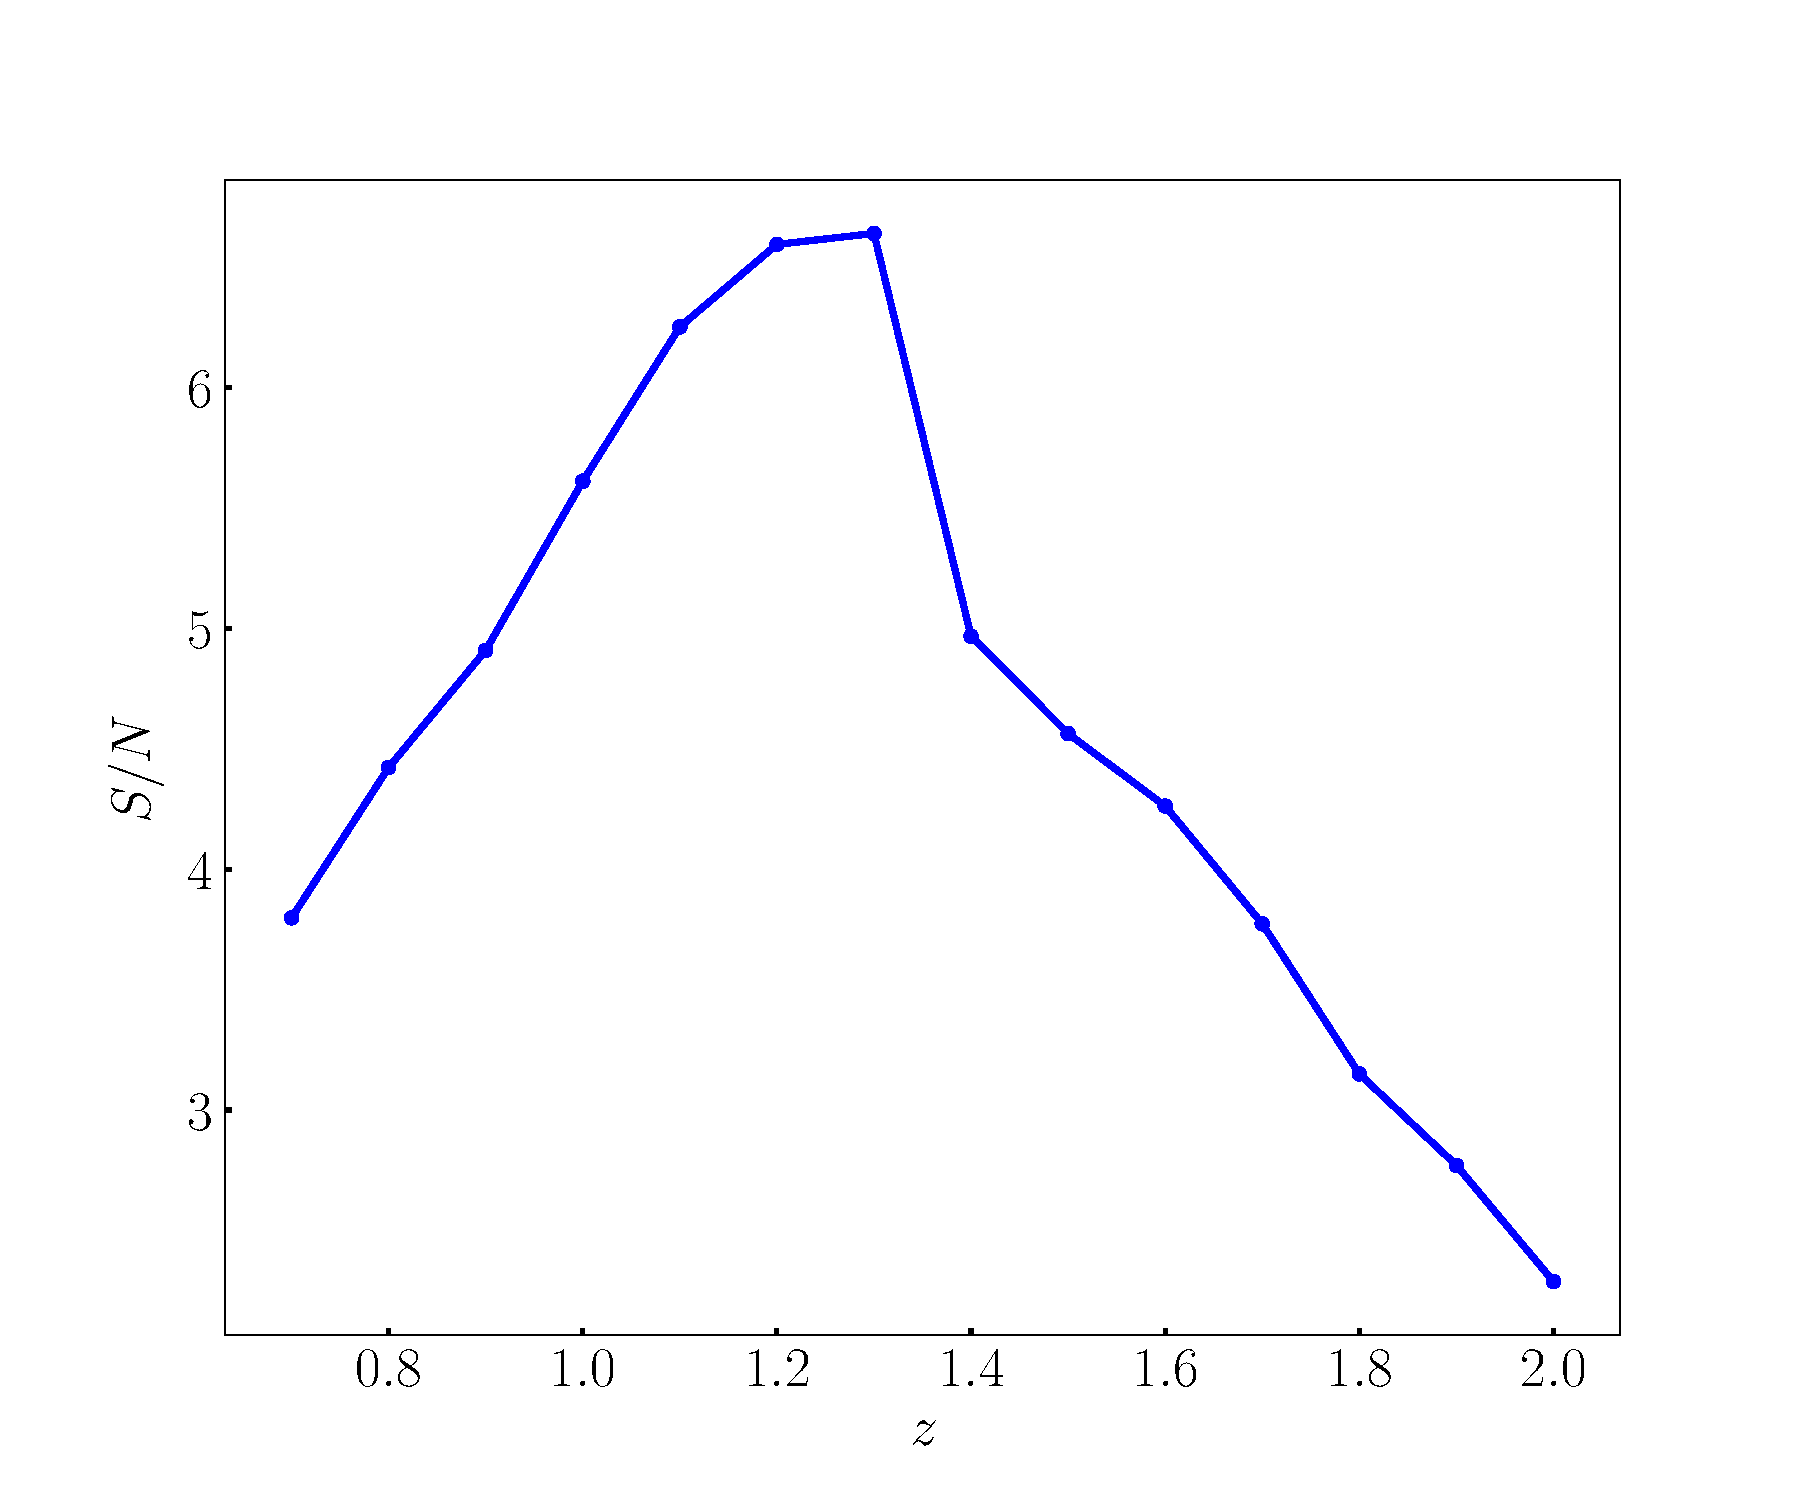
\includegraphics[width=7.5cm]{fig/snrDoppler-eps-converted-to}
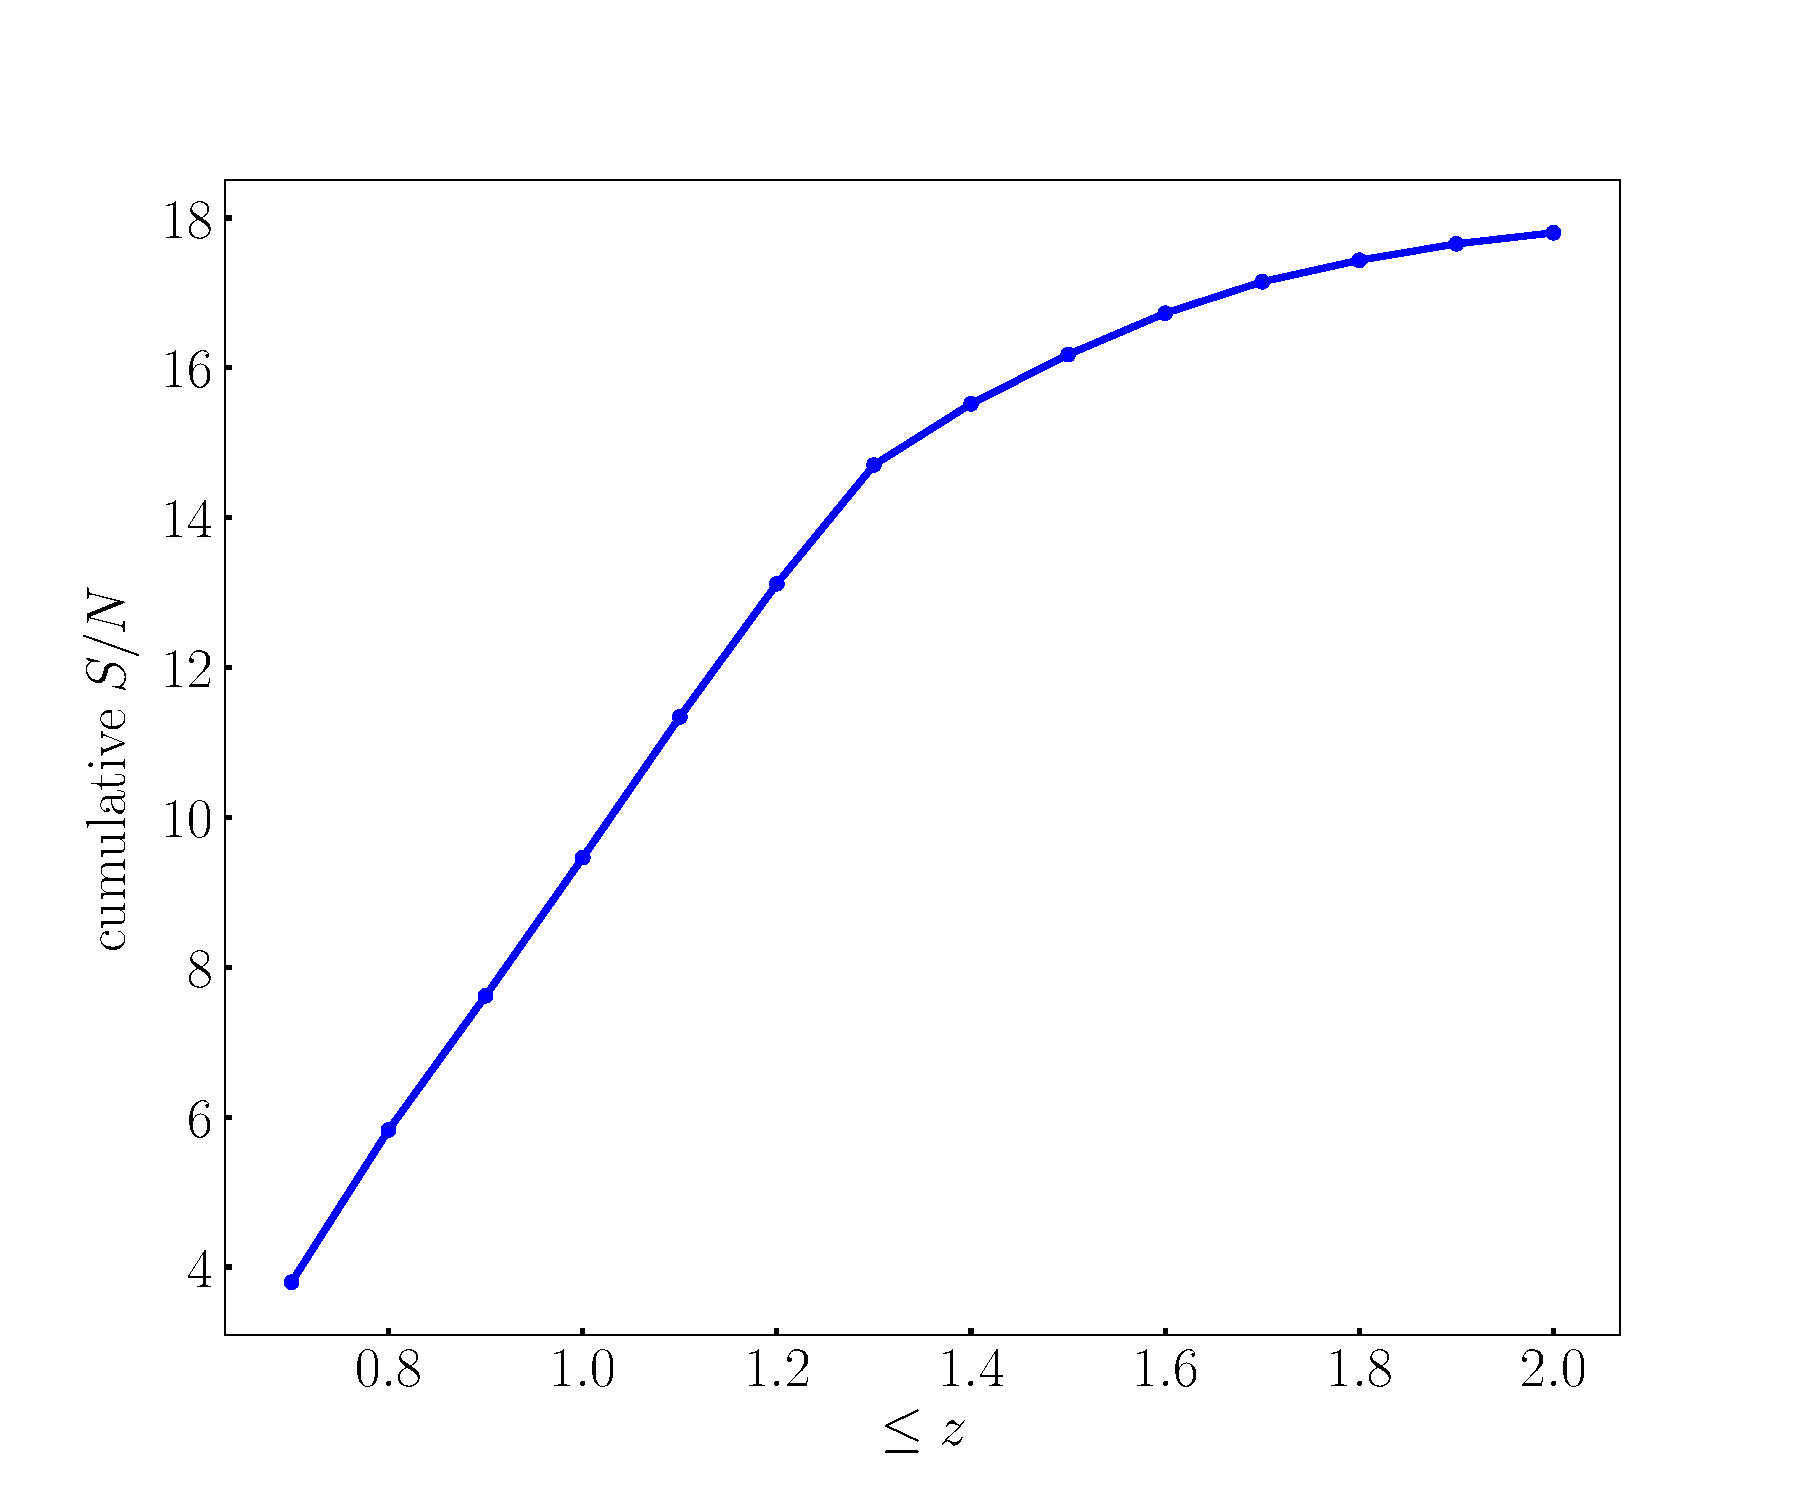
\includegraphics[width=7.5cm]{fig/CumulativesnrDoppler-eps-converted-to}
\caption{Relativistic SNR per $z$-bin  ({\em left}) and cumulative ({\em right}) for a Stage IV $H\alpha$ survey.} \label{fig4}
\end{figure}
\begin{figure}[ht]
\centering
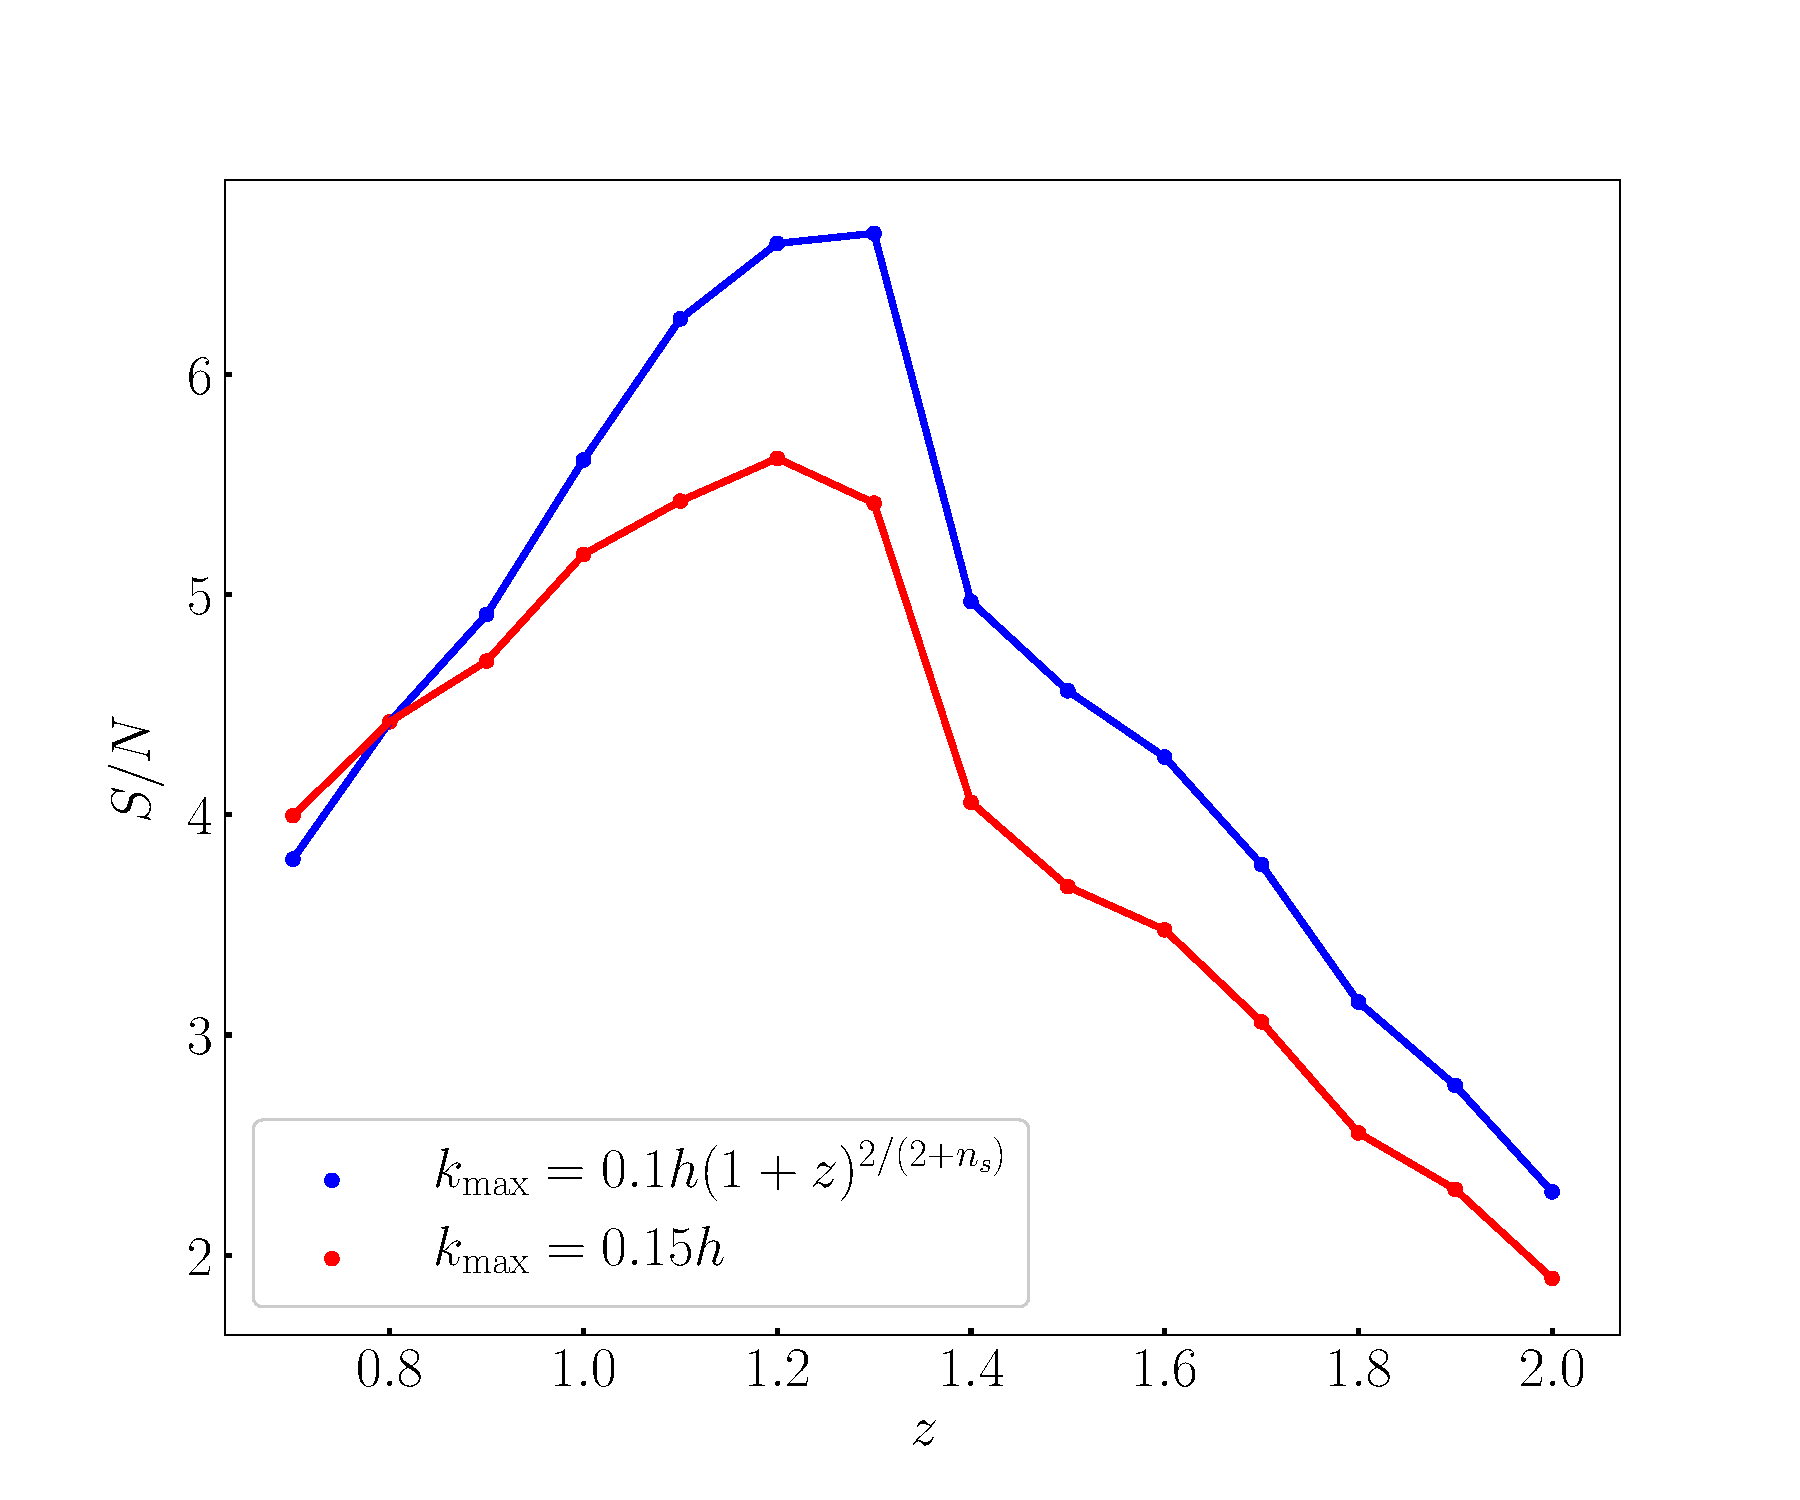
\includegraphics[width=7.5cm]{fig/kmaxsnr-eps-converted-to}
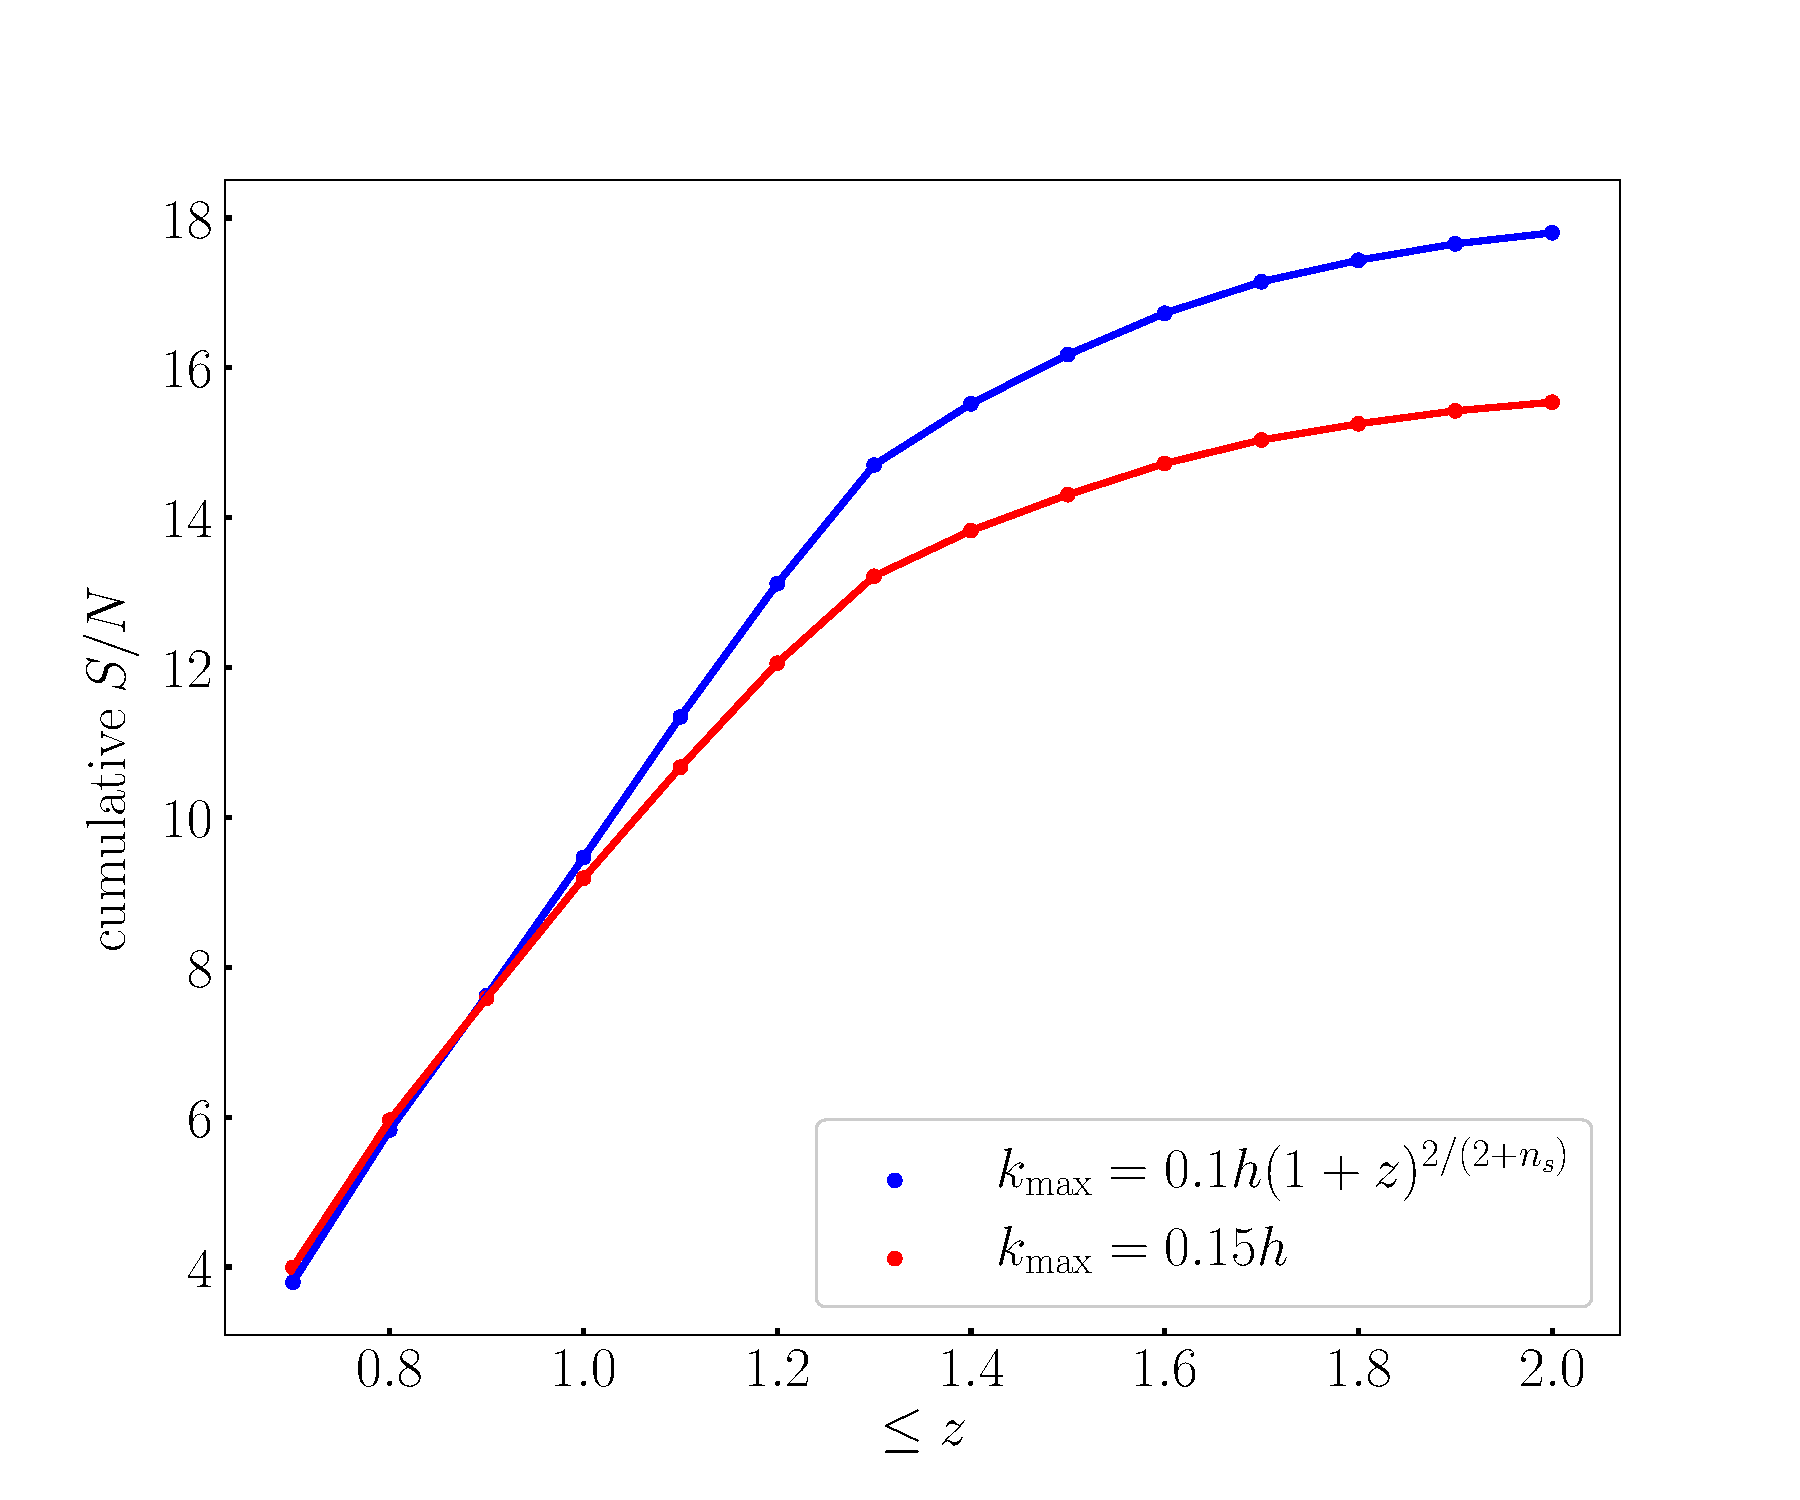
\includegraphics[width=7.5cm]{fig/kmaxcumsnr-eps-converted-to} 
\caption{Effect of changing $k_{\mathrm{max}}$ on SNR per bin ({\em left}) and cumulative SNR ({\em right}).} \label{kmsnr}
\end{figure} 
\item  
Changes in $b_e(z),\Q(z)$: 
The effect on the relativistic SNR of changes in magnification bias and in evolution bias is illustrated in Fig.~\ref{fig1x}.
\begin{figure}[ht]
\centering
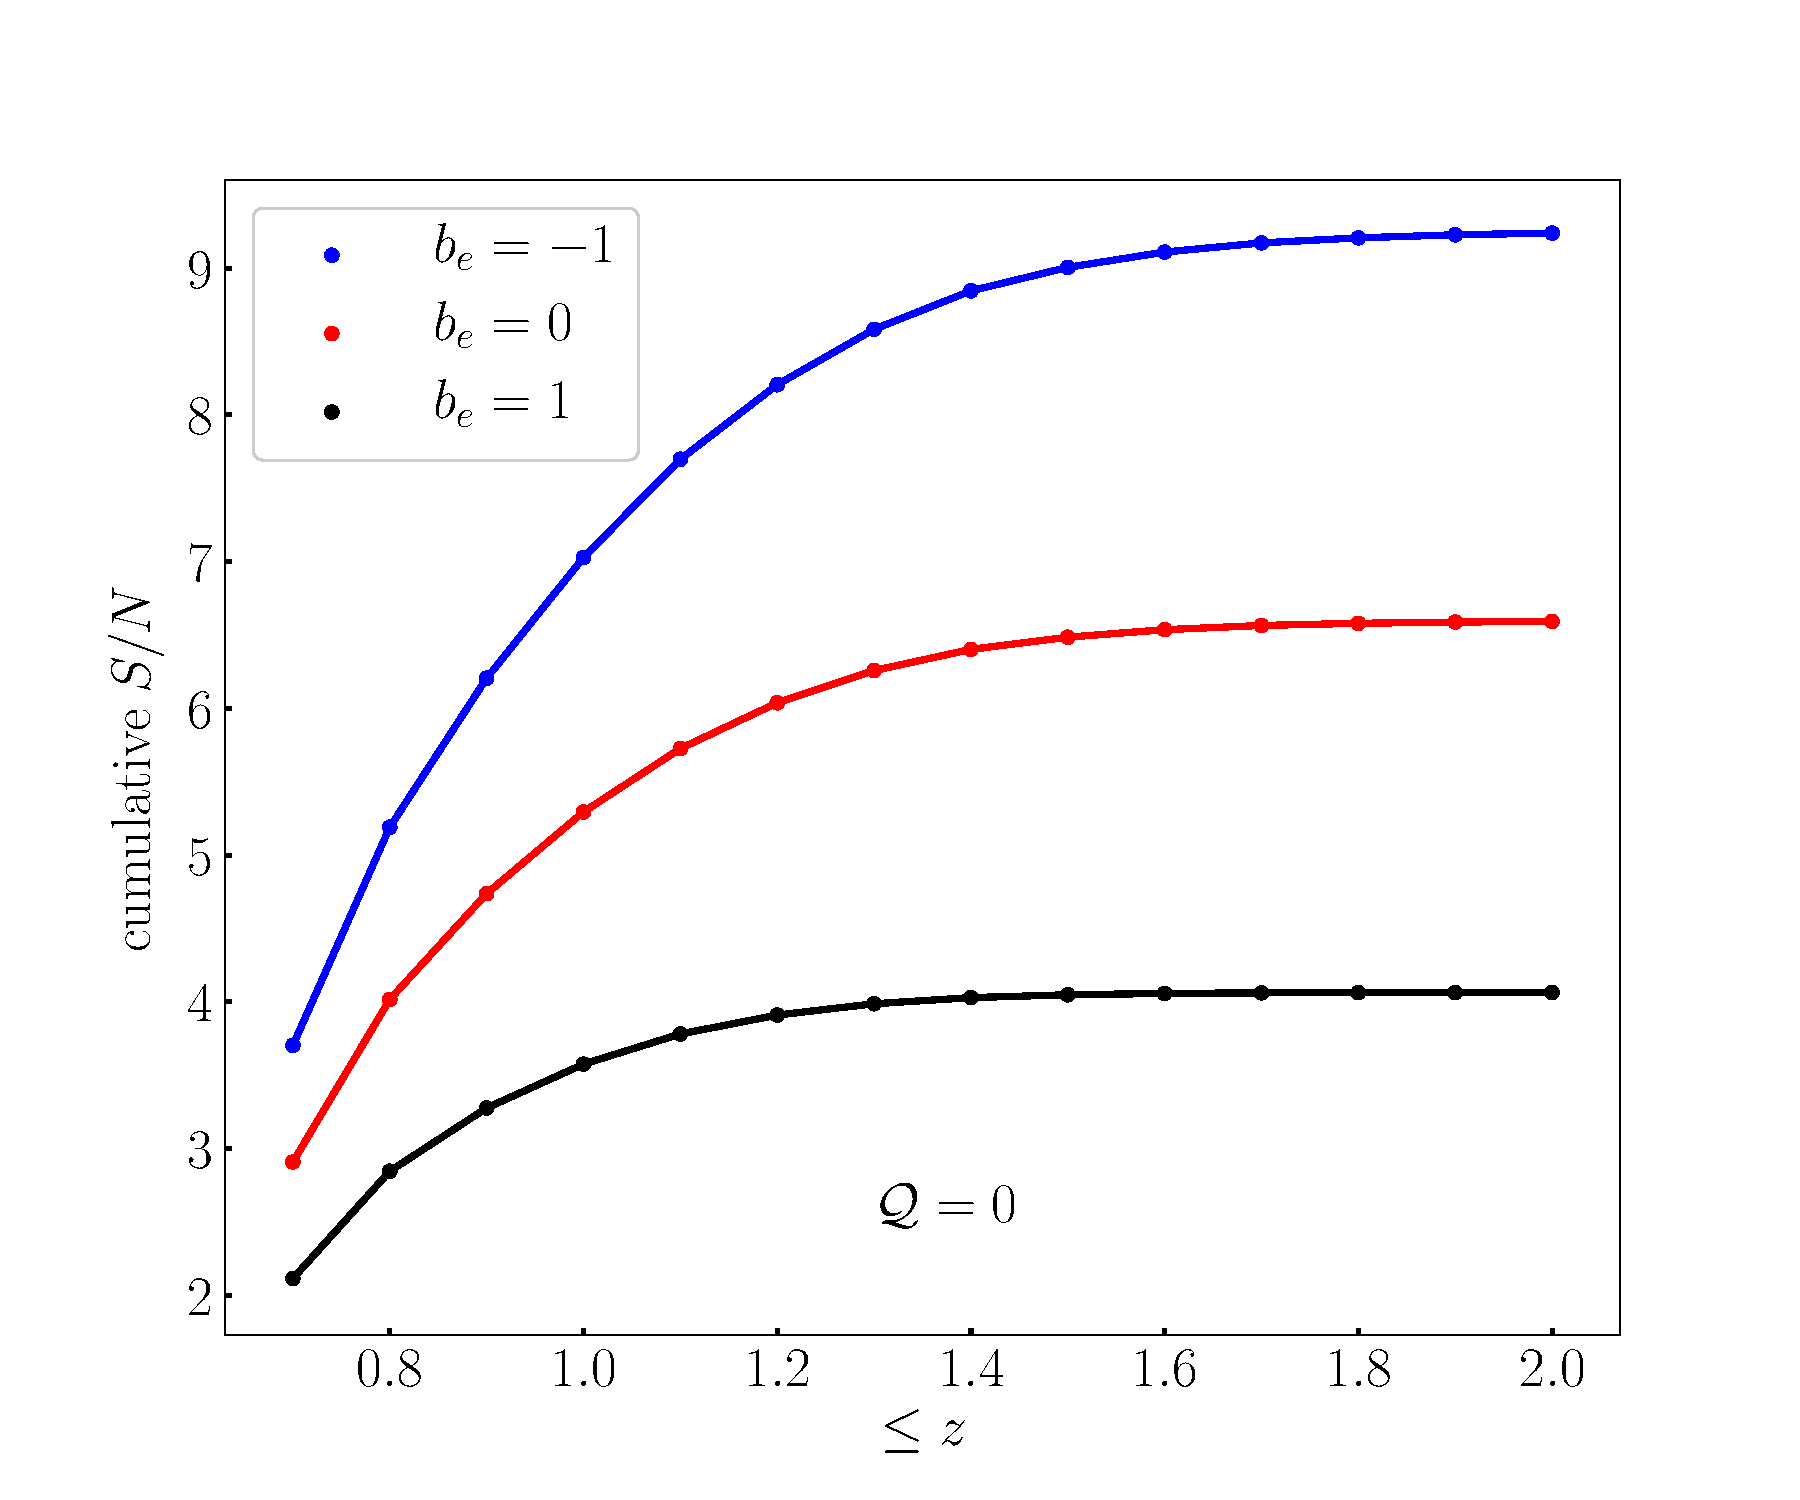
\includegraphics[width=7cm]{fig/cumulativeSnrdopplerQ0_0-eps-converted-to} 
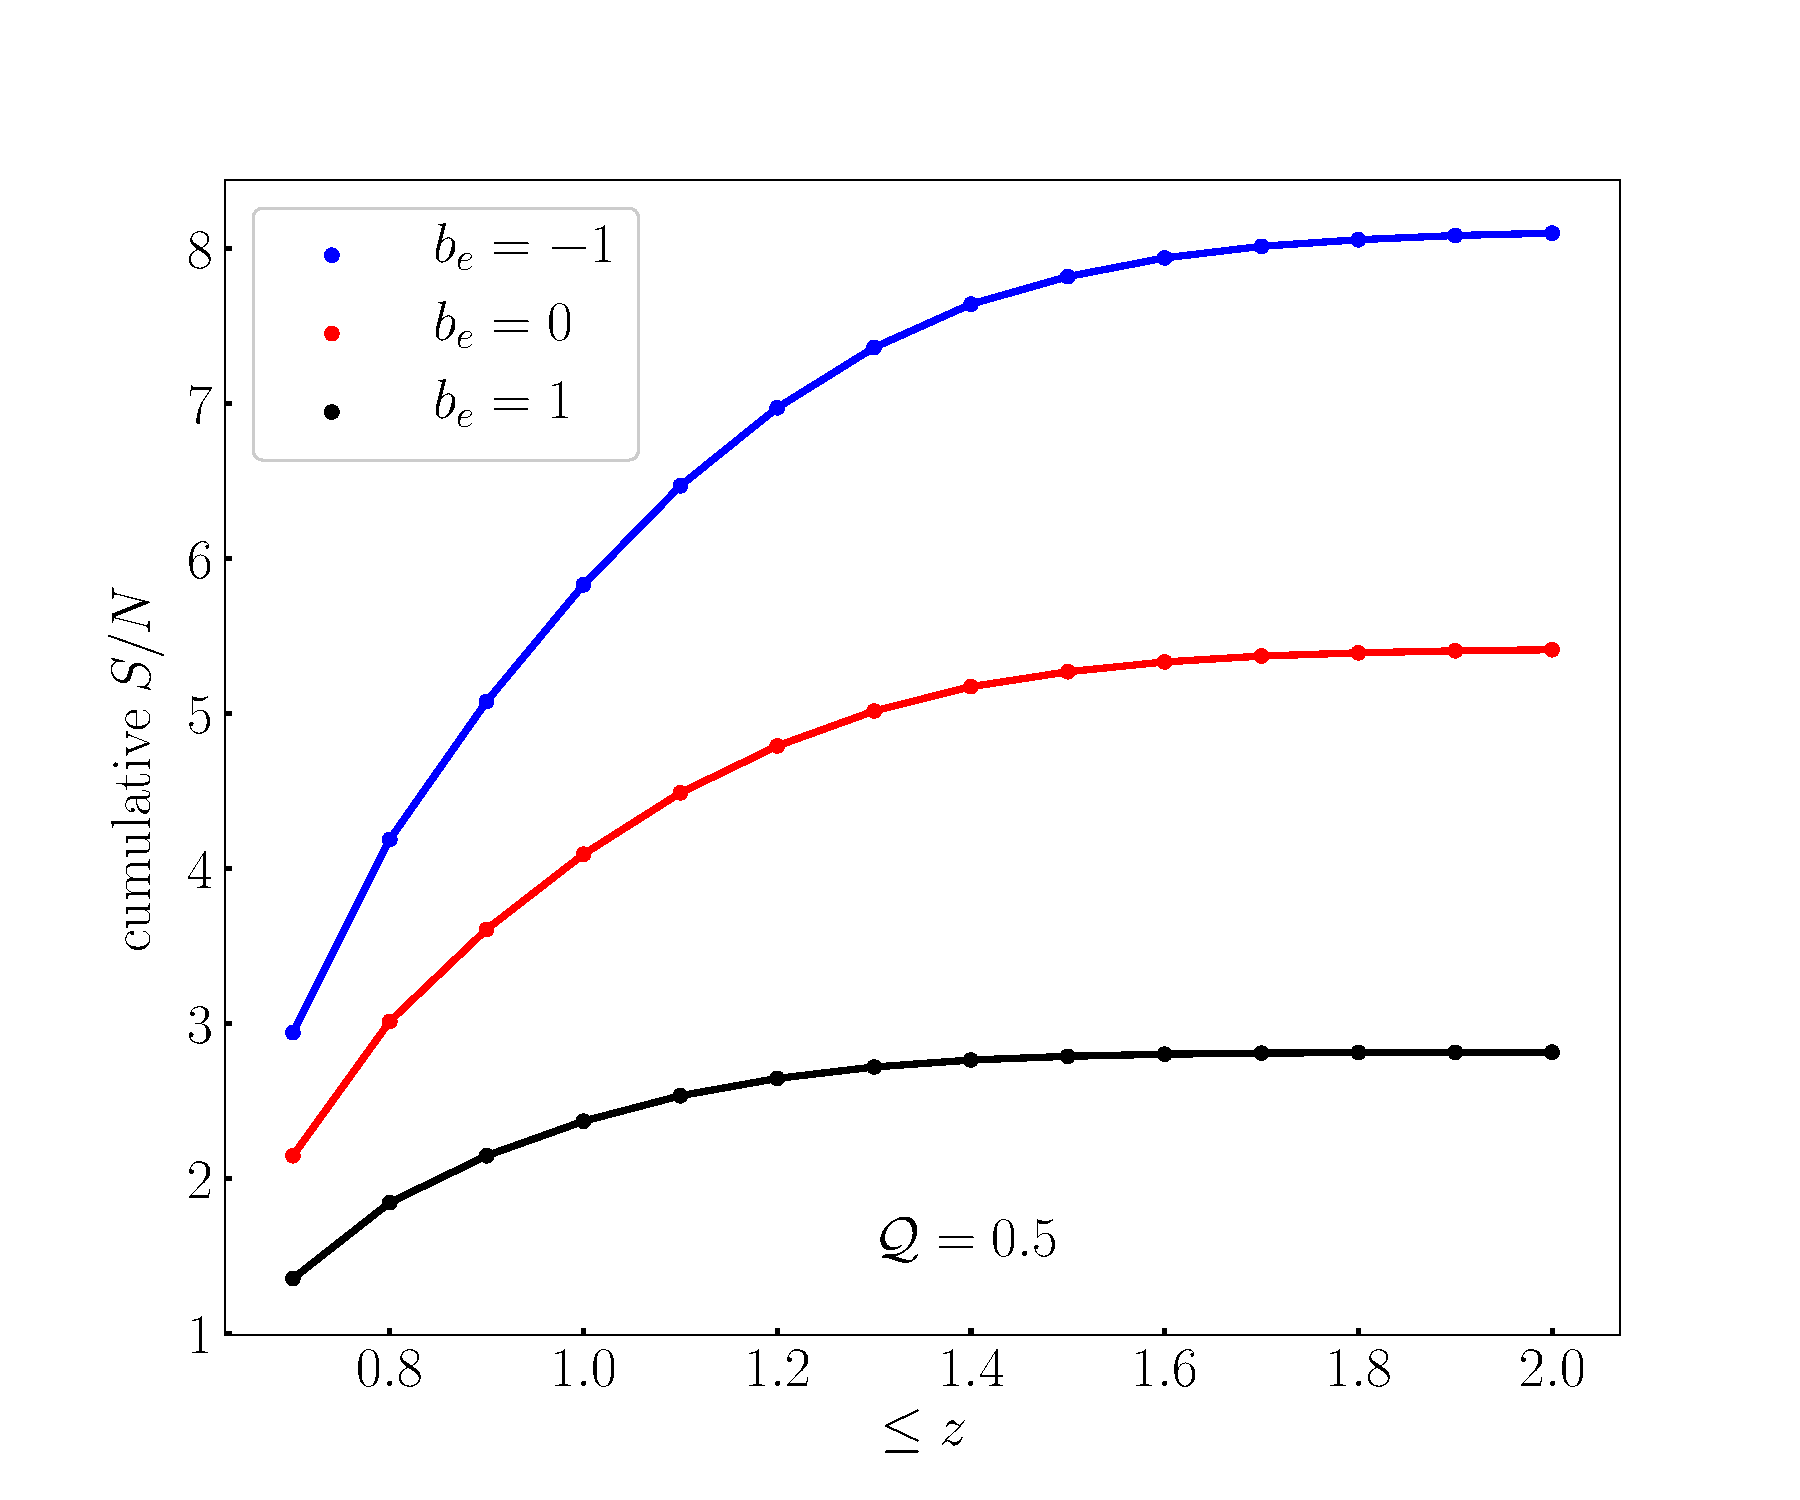
\includegraphics[width=7cm]{fig/cumulativeSnrdopplerQ0_5-eps-converted-to} \\
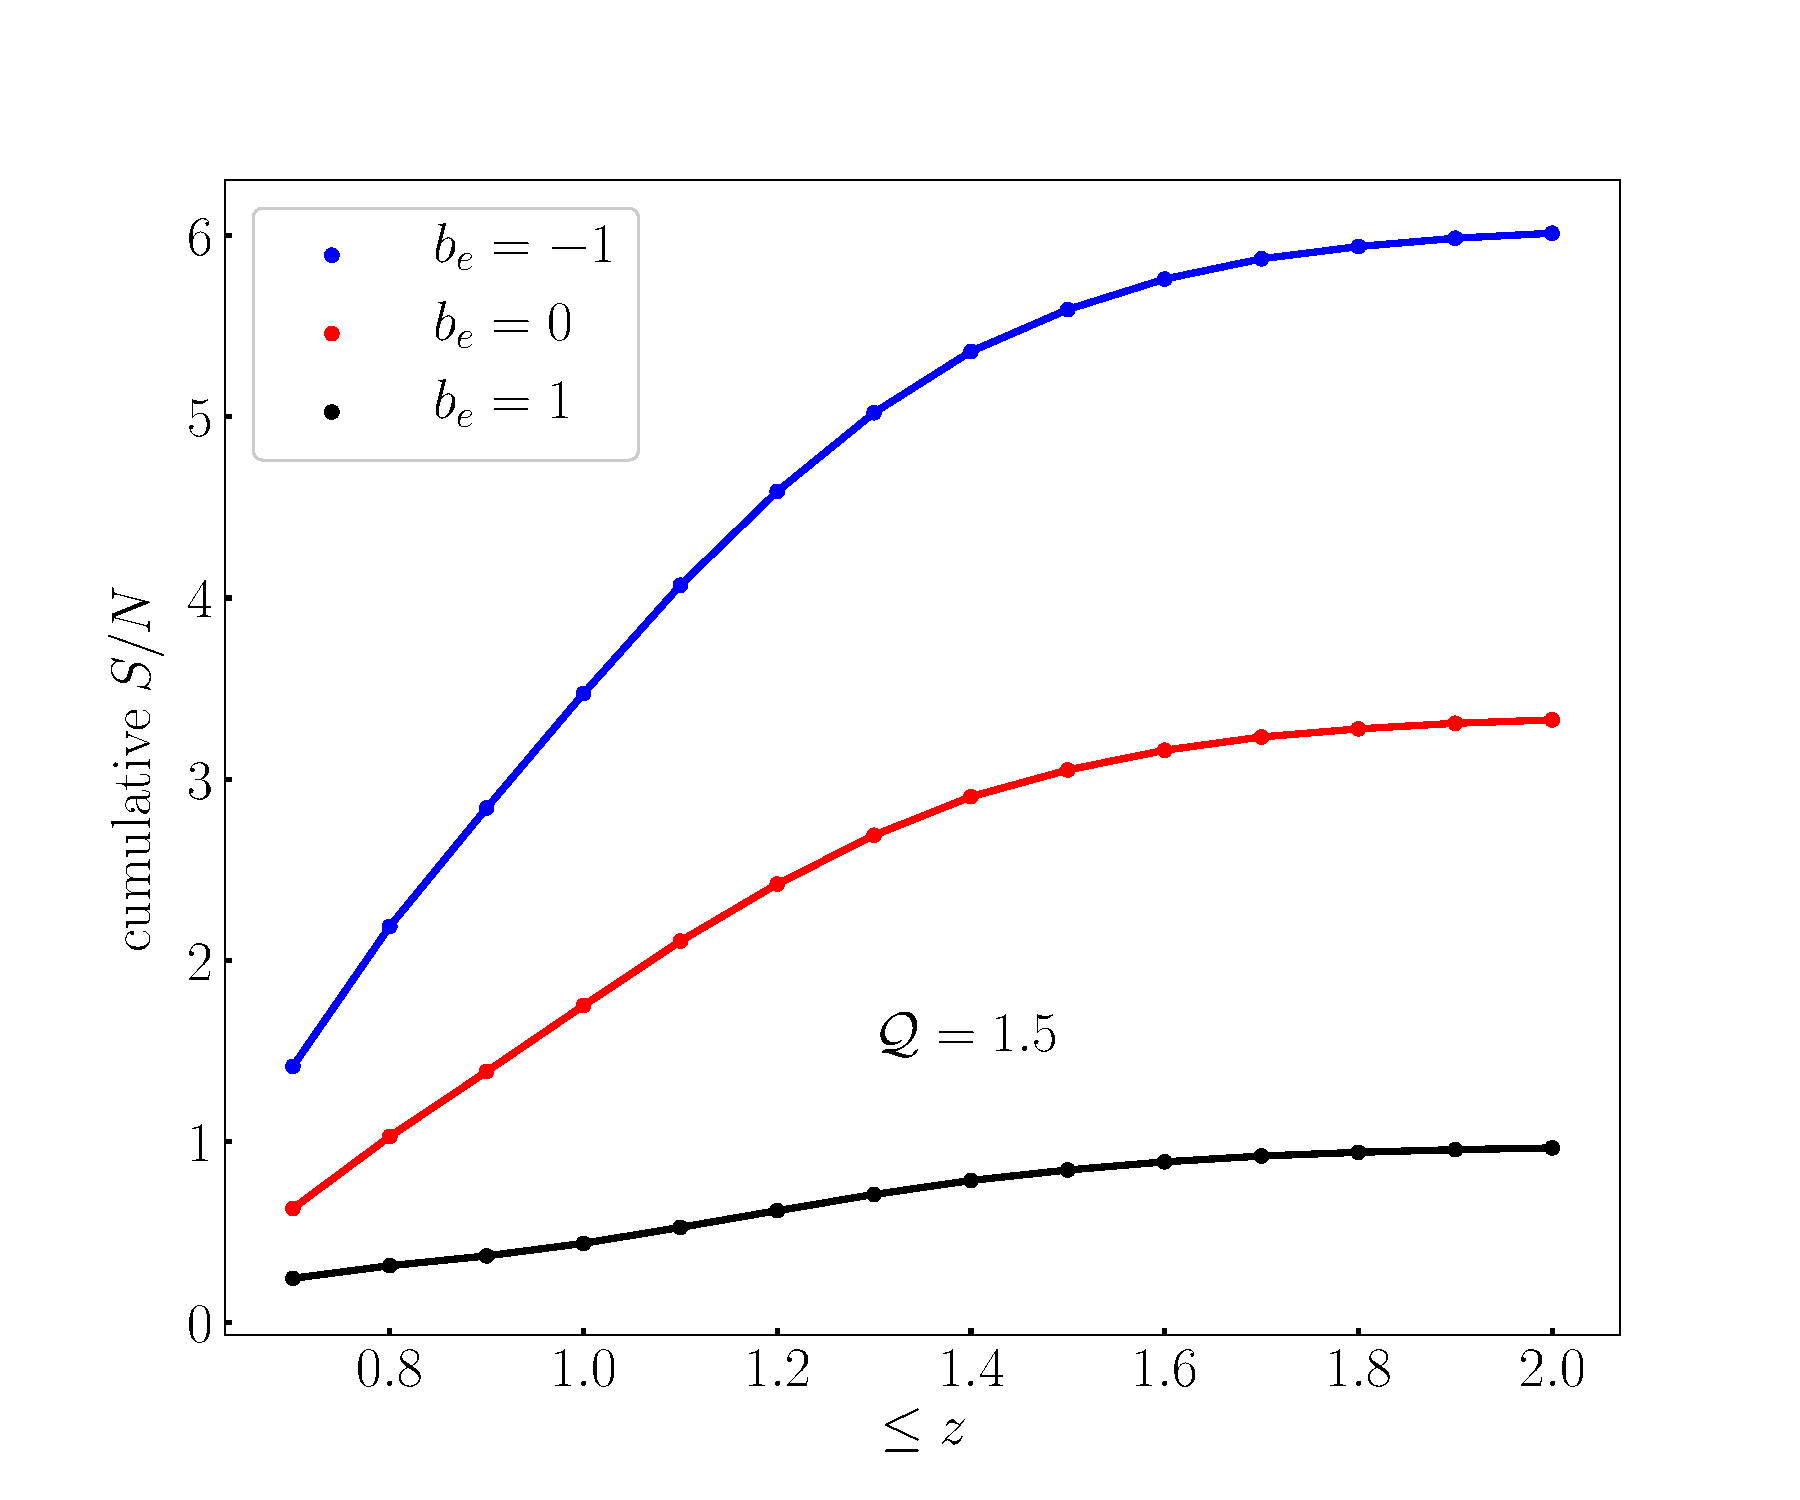
\includegraphics[width=7cm]{fig/cumulativeSnrdopplerQ1_5-eps-converted-to}
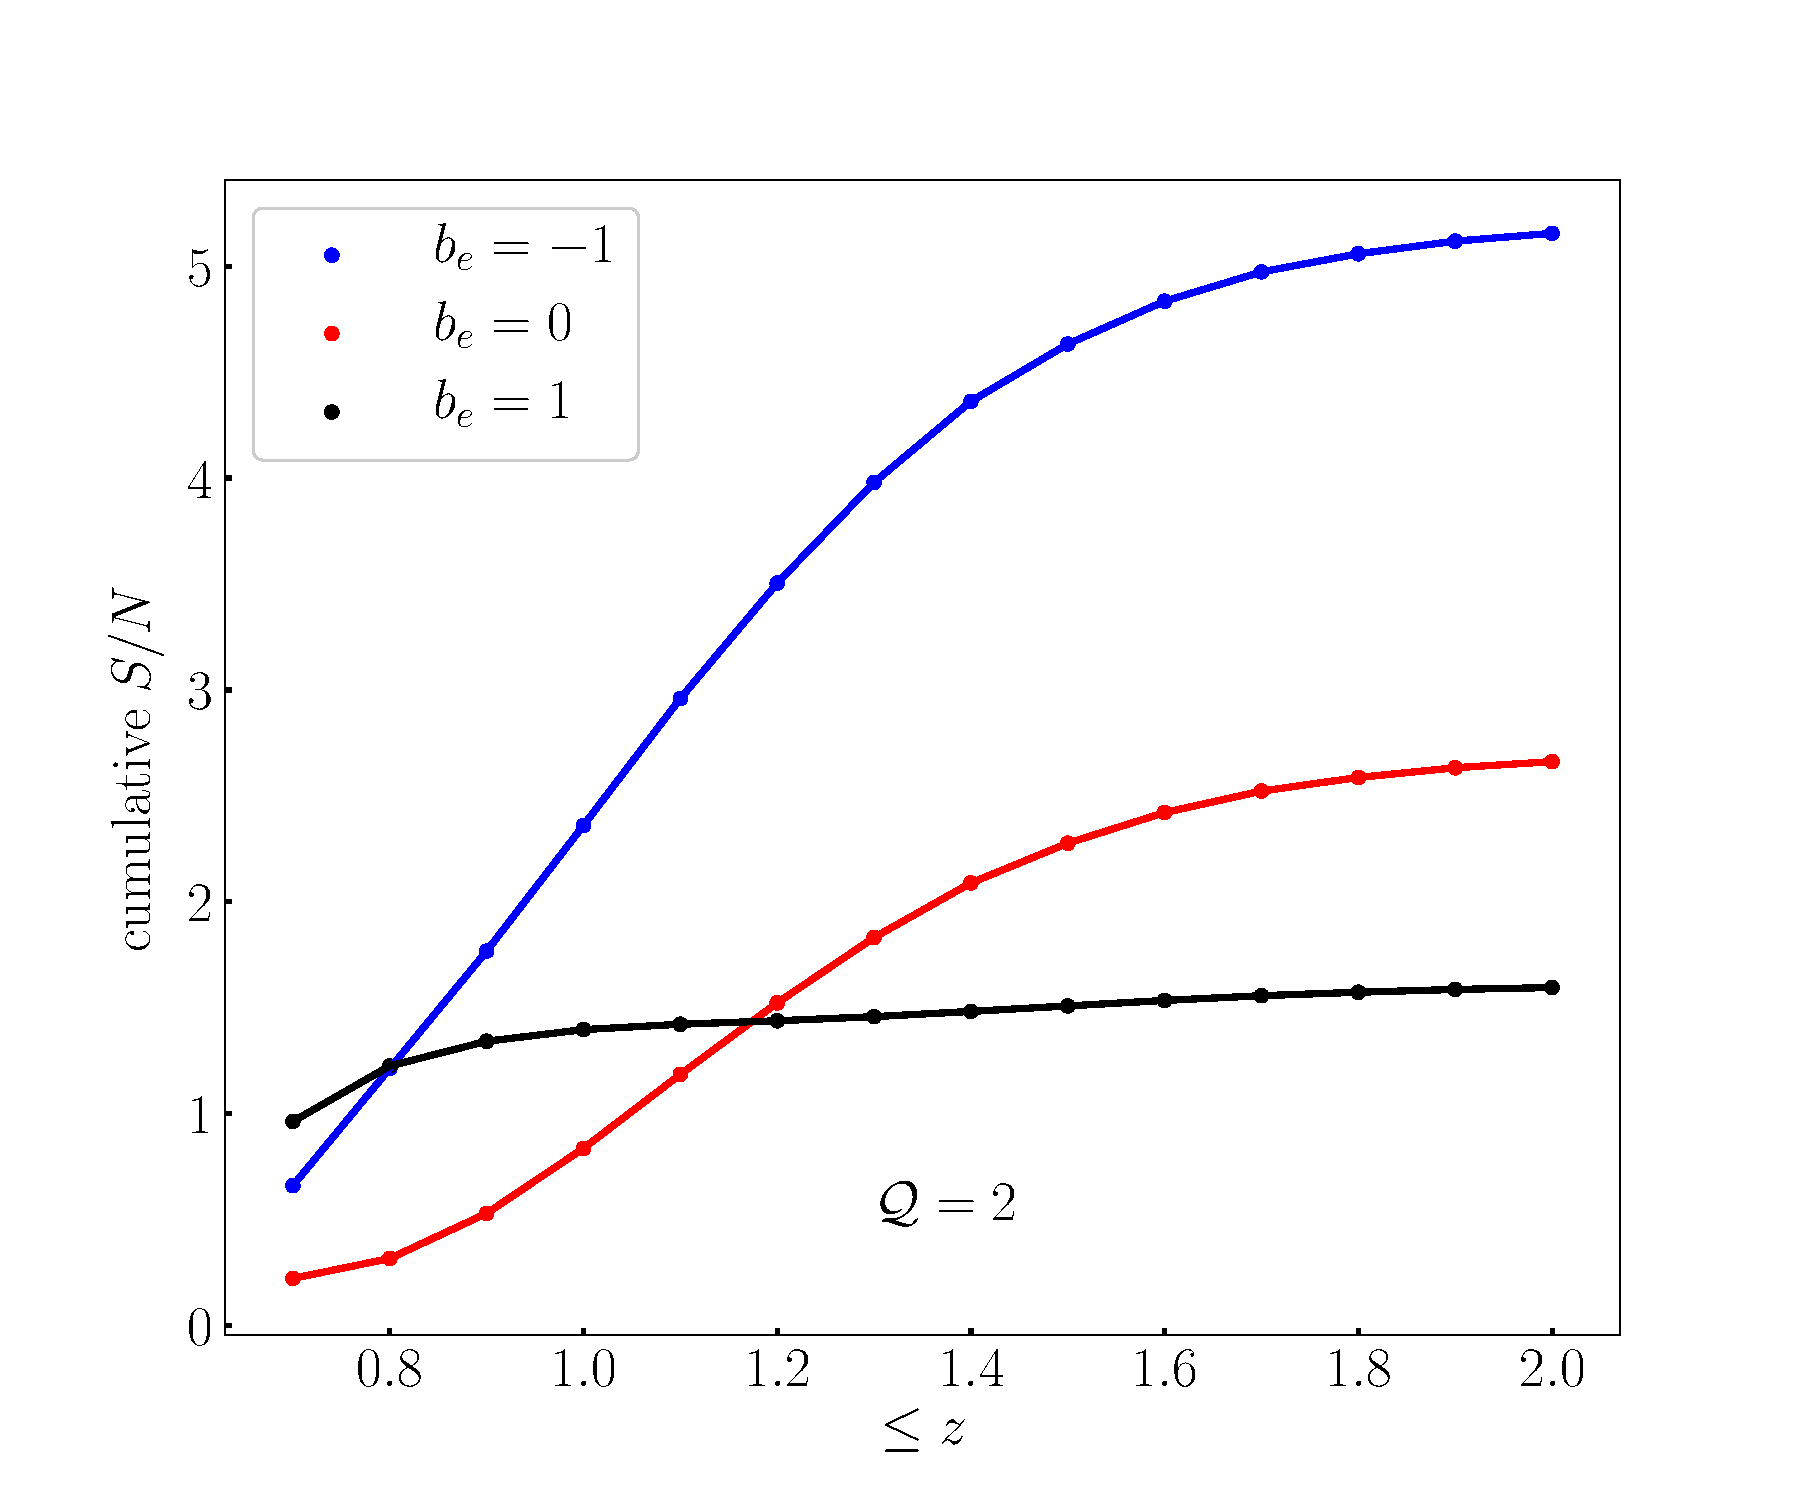
\includegraphics[width=7cm]{fig/cumulativeSnrdopplerQ2_0-eps-converted-to} 
\caption{Effect of changing ${\cal Q}$ and $b_e$ on relativistic cumulative SNR.} \label{fig1x}
\end{figure}
In Figure~\ref{fig1x}) we illustrate the significant impact on cumulative SNR of changing $b_e,\Q$. We use a range of constant choices for $b_e,\Q$ -- which are not physically motivated. This shows the importance of modelling $b_e,\Q$ self-consistently from the same  luminosity function that produces the number density, as we have done. 
\end{itemize}

{The sensitivity of the relativistic SNR to  $k_{\mathrm{max}}$ reflects the importance of the coupling of the relativistic signal to Newtonian terms on short scales. How sensitive is the SNR to the signal on the largest scales? We can answer this by increasing $k_{\mathrm{min}}$ from its fiducial value $k_{\mathrm{f}}$, which is the maximal observable scale. The result is that there is only a small reduction when $k_{\mathrm{min}}/k_{\mathrm{f}}$ is increased by a factor up to 5, as shown in Fig.~\ref{kmin}. 
{Even with $k_{\mathrm{min}}=10 k_{\mathrm{f}}$, the total SNR is $\sim 10$.} 
This means that the relativistic SNR does not depend critically on accessing the largest possible scales.}
\begin{figure}[ht]
\centering
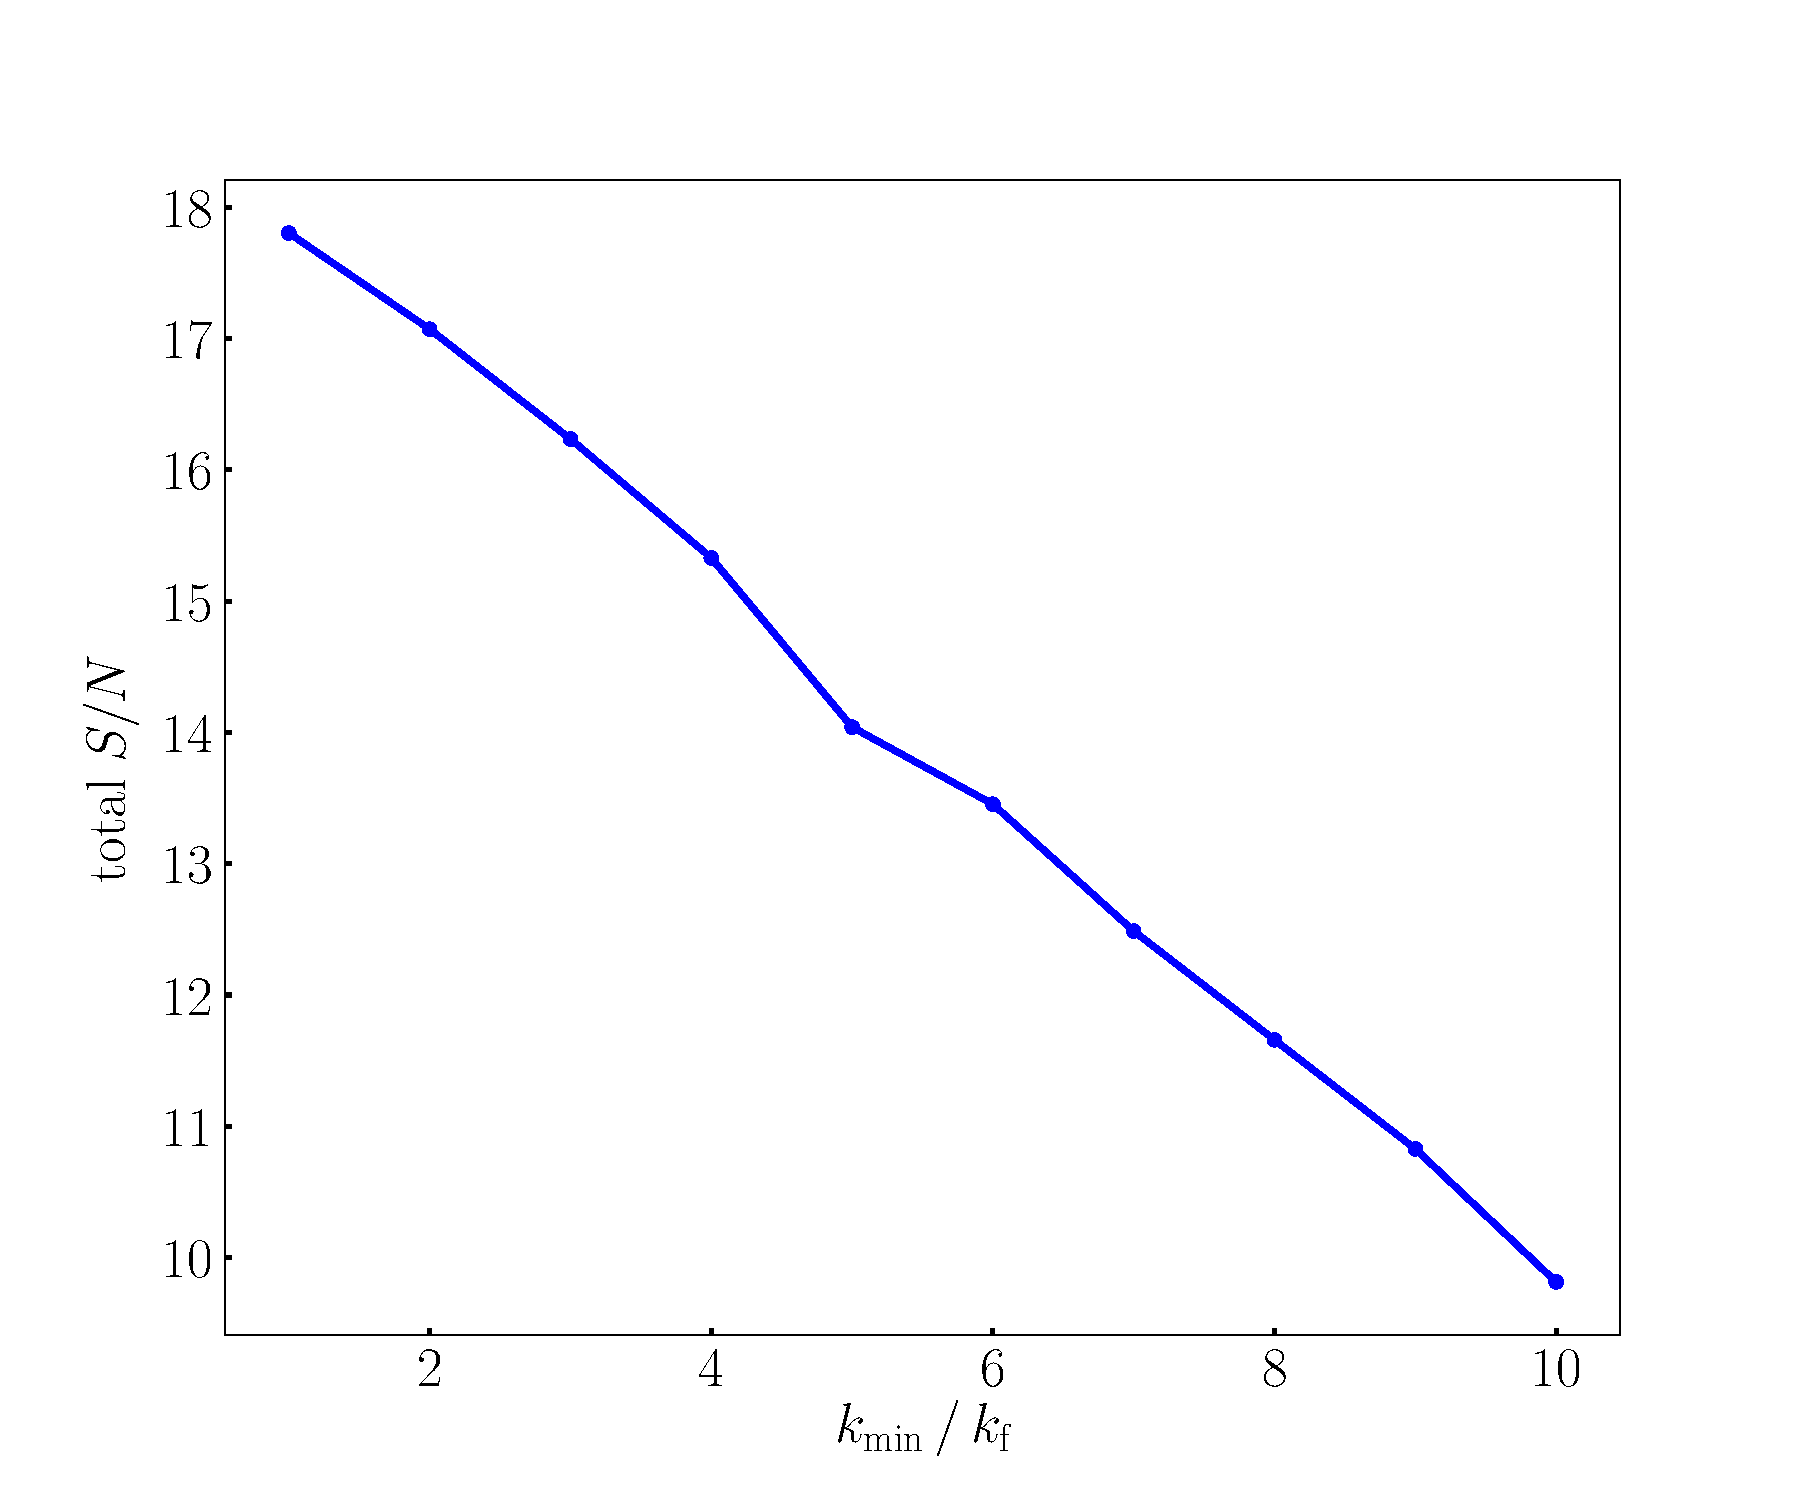
\includegraphics[width=8.0cm]{fig/cumDoppSnr_kmin-eps-converted-to}
\caption{{Effect of changing $k_{\mathrm{min}}$ on  total relativistic SNR.} 
} \label{kmin}
\end{figure} 

It is also interesting to investigate how important for the SNR is the second-order relativistic contribution 
in the bispectrum, i.e. from terms of the form
\begin{equation} \label{2oc}
\mathcal{K}^{(1)}_{\mathrm{N}}(\bm{k}_{1})\mathcal{K}^{(1)}_{\mathrm{N}}(\bm{k}_{2})\mathcal{K}^{(2)}_{\mathrm{D}}(\bm{k}_{1},\bm{k}_{2},\bm{k}_{3})\,,
\end{equation}
 in \eqref{e21},  compared to the first-order contribution, i.e. from terms of the form
 \begin{equation} \label{1oc}
 \Big[\mathcal{K}^{(1)}_{\mathrm{N}}(\bm{k}_{1})\mathcal{K}^{(1)}_{\mathrm{D}}(\bm{k}_{2}) + \mathcal{K}^{(1)}_{\mathrm{D}}(\bm{k}_{1})\mathcal{K}^{(1)}_{\mathrm{N}}(\bm{k}_{2})\Big]\mathcal{K}^{(2)}_{\mathrm{N}}(\bm{k}_{1},\bm{k}_{2},\bm{k}_{3}) \,.
 \end{equation}
 It is conceivable that the first-order Doppler-type contribution in \eqref{1oc} to $B_g$, which couples to first- and second-order Newtonian terms, dominates the SNR. However, we find that the first- and  second-order relativistic parts of the bispectrum make comparable contributions to the SNR -- see Fig.~\ref{fig4z}. We deduce that the second-order relativistic contribution in \eqref{2oc} cannot be neglected. Furthermore, this means that it must be accurately modelled, as we  have done. 
\begin{figure}[ht]
\centering
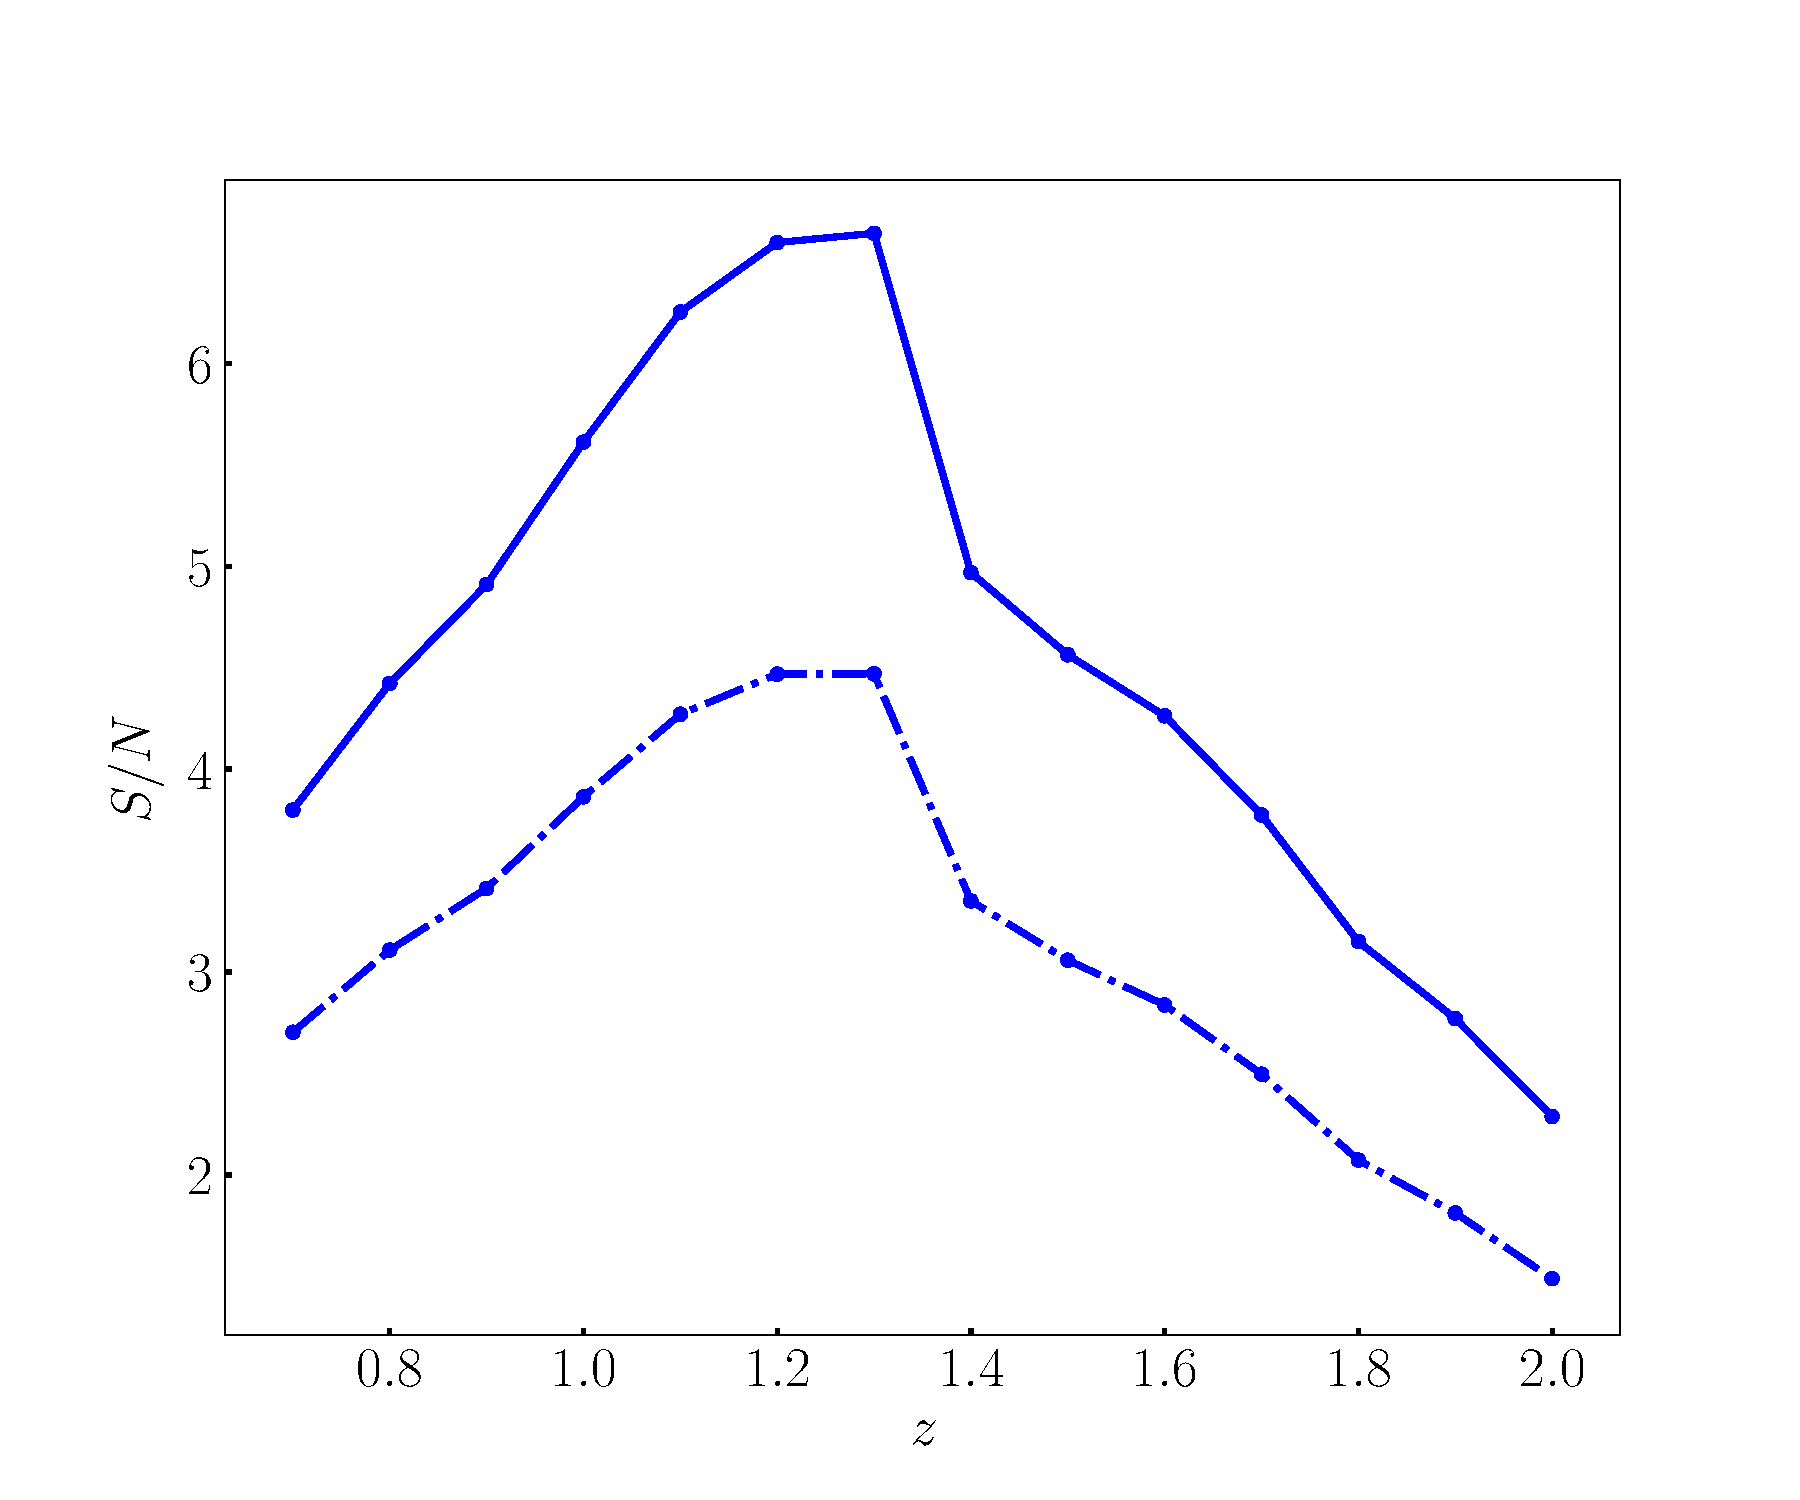
\includegraphics[width=7.5cm]{fig/DoppSnr_K2D-eps-converted-to}
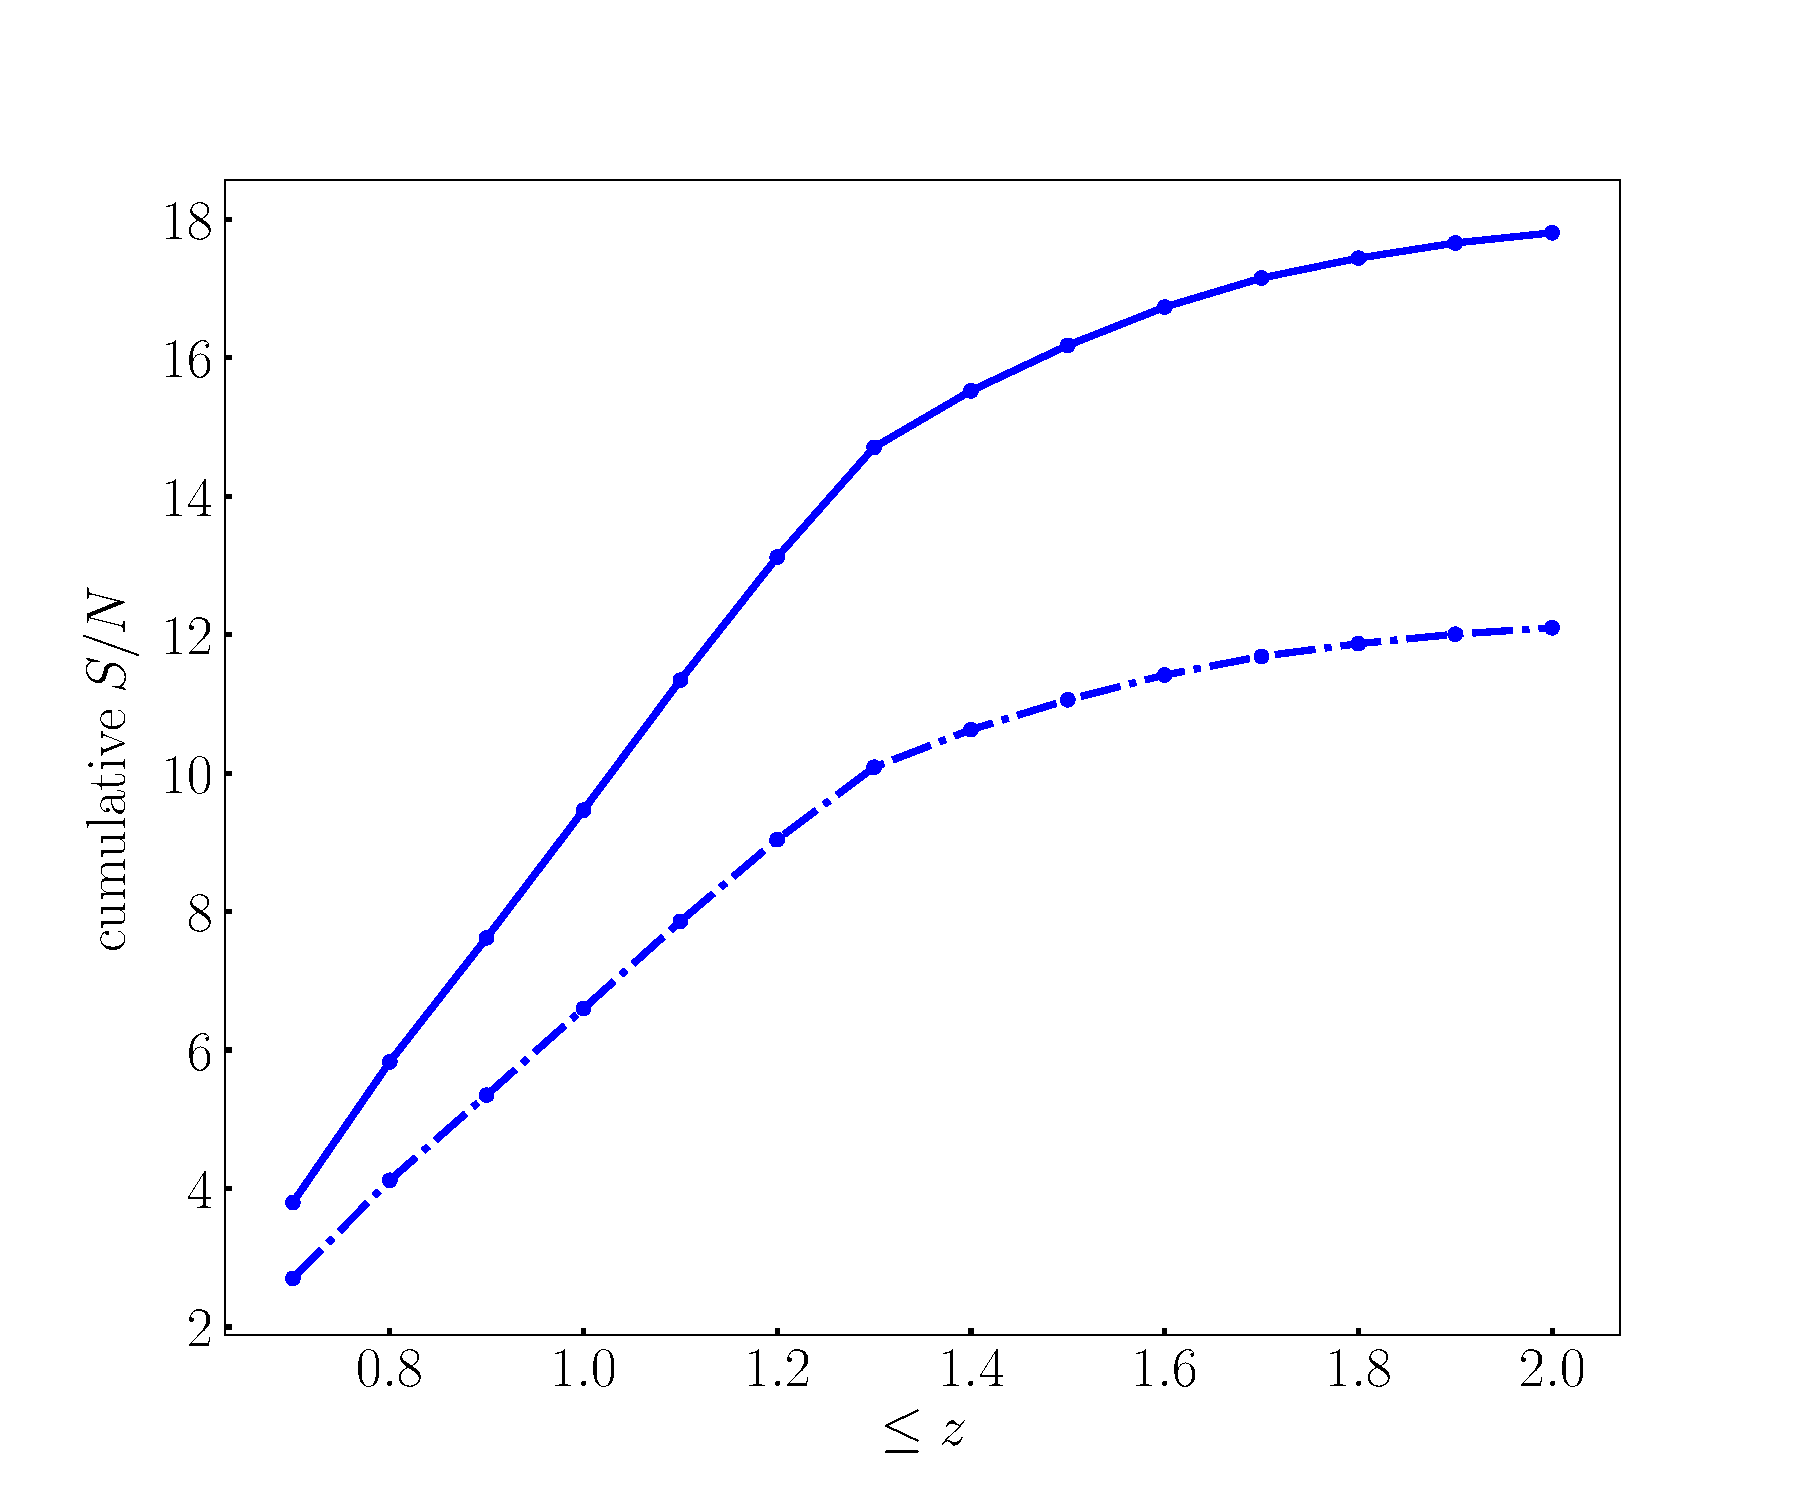
\includegraphics[width=7.5cm]{fig/cumDoppSnr_K2D-eps-converted-to}
\caption{As in Fig.~\ref{fig4}, but showing the effect of omitting the second-order relativistic contribution \eqref{2oc} to the bispectrum (dot-dashed curves).} \label{fig4z}
\end{figure}

Recently \cite{Jeong:2019igb} estimated the  SNR for the leading relativistic part of the bispectrum.  There are significant differences in their analysis compared to ours. In particular, they neglect most of the terms in $\delta_{g \mathrm{D}}^{(2)}$ [see our \eqref{dg2}] which defines ${\cal K}^{(2)}_{\mathrm{D}}$ 
In \cite{Jeong:2019igb},  
a significant number of terms is neglected in the relativistic second-order  galaxy number count contrast, $\delta_{g\mathrm{D}}^{(2)}$, given by our \eqref{dg2}. (Note that our  \eqref{dg2}, derived in \cite{Clarkson:2018dwn}, was independently confirmed by \cite{DiDio:2018zmk}). They have the first term, $A\, \bm{v}^{(2)}\!\!\cdot\bm{n}$, on the right of \eqref{dg2}.  In the second term, $2{C}(\bm{v}\cdot\bm{n})\,\delta$, they do not have the correct form of the coefficient $C$ -- they include only the first part, $b_1A$, of $C$ [see the right-hand side of eq 26?]. All terms after the second term in \eqref{dg2} are omitted by \cite{Jeong:2019igb}. Note that none of the omitted terms is suppressed by a higher power of $k^{-1}$;  they all have the same scaling, i.e., $\propto (\cH/k)\,{(\delta)^2}$. In detail, they omit the following
terms:
\begin{align}
\delta_{g\mathrm{D}}^{(2)}({\mathrm{us}})- \delta_{g\mathrm{D}}^{(2)}(\mbox{{\cite{Jeong:2019igb}}}) &= 2\left[b_{1}f + \frac{b_1'}{\cH} 
+ 2\bigg(1-\frac{1}{{r} \cH}\bigg){\frac{\partial b_1}{\partial \ln{L}}\bigg|_{\mathrm{c}}} \right](\bm{v}\cdot\bm{n})\,\delta 
\\\nonumber
& 
+ \frac{2}{\cH}\left(4-2A-\frac{3}{2}\Omega_{m} \right)(\bm{v}\cdot\bm{n})\,\partial_r(\bm{v}\cdot\bm{n})\\
\nonumber
&
+ \frac{2}{\cH^2}\big[(\bm{v}\cdot\bm{n}) \,\partial_r^2\Phi-\Phi\, \partial_r^2 (\bm{v}\cdot\bm{n}) \big]
 - \frac{2}{\cH}\,\partial_r (\bm{v}\cdot\bm{v}) + 2 \frac{b_1}{\cH}\,\Phi\, \partial_r\delta \,. 
\end{align} In addition they do not use self-consistent models for $b_{e}$ and $\mathcal{Q}$. These two differences could account for their conclusion that the relativistic signal is not detectable, in contrast to our result. 


An interesting feature of the relativistic signal is that there is a significant contribution to the SNR from  flattened triangle shapes. This is consistent with the results of  \cite{Clarkson:2018dwn} for the dipole that is generated by the imaginary part of the bispectrum.
%
%

\subsection{Inclusion of cosmological parameters}
\begin{figure}[ht]
\centering
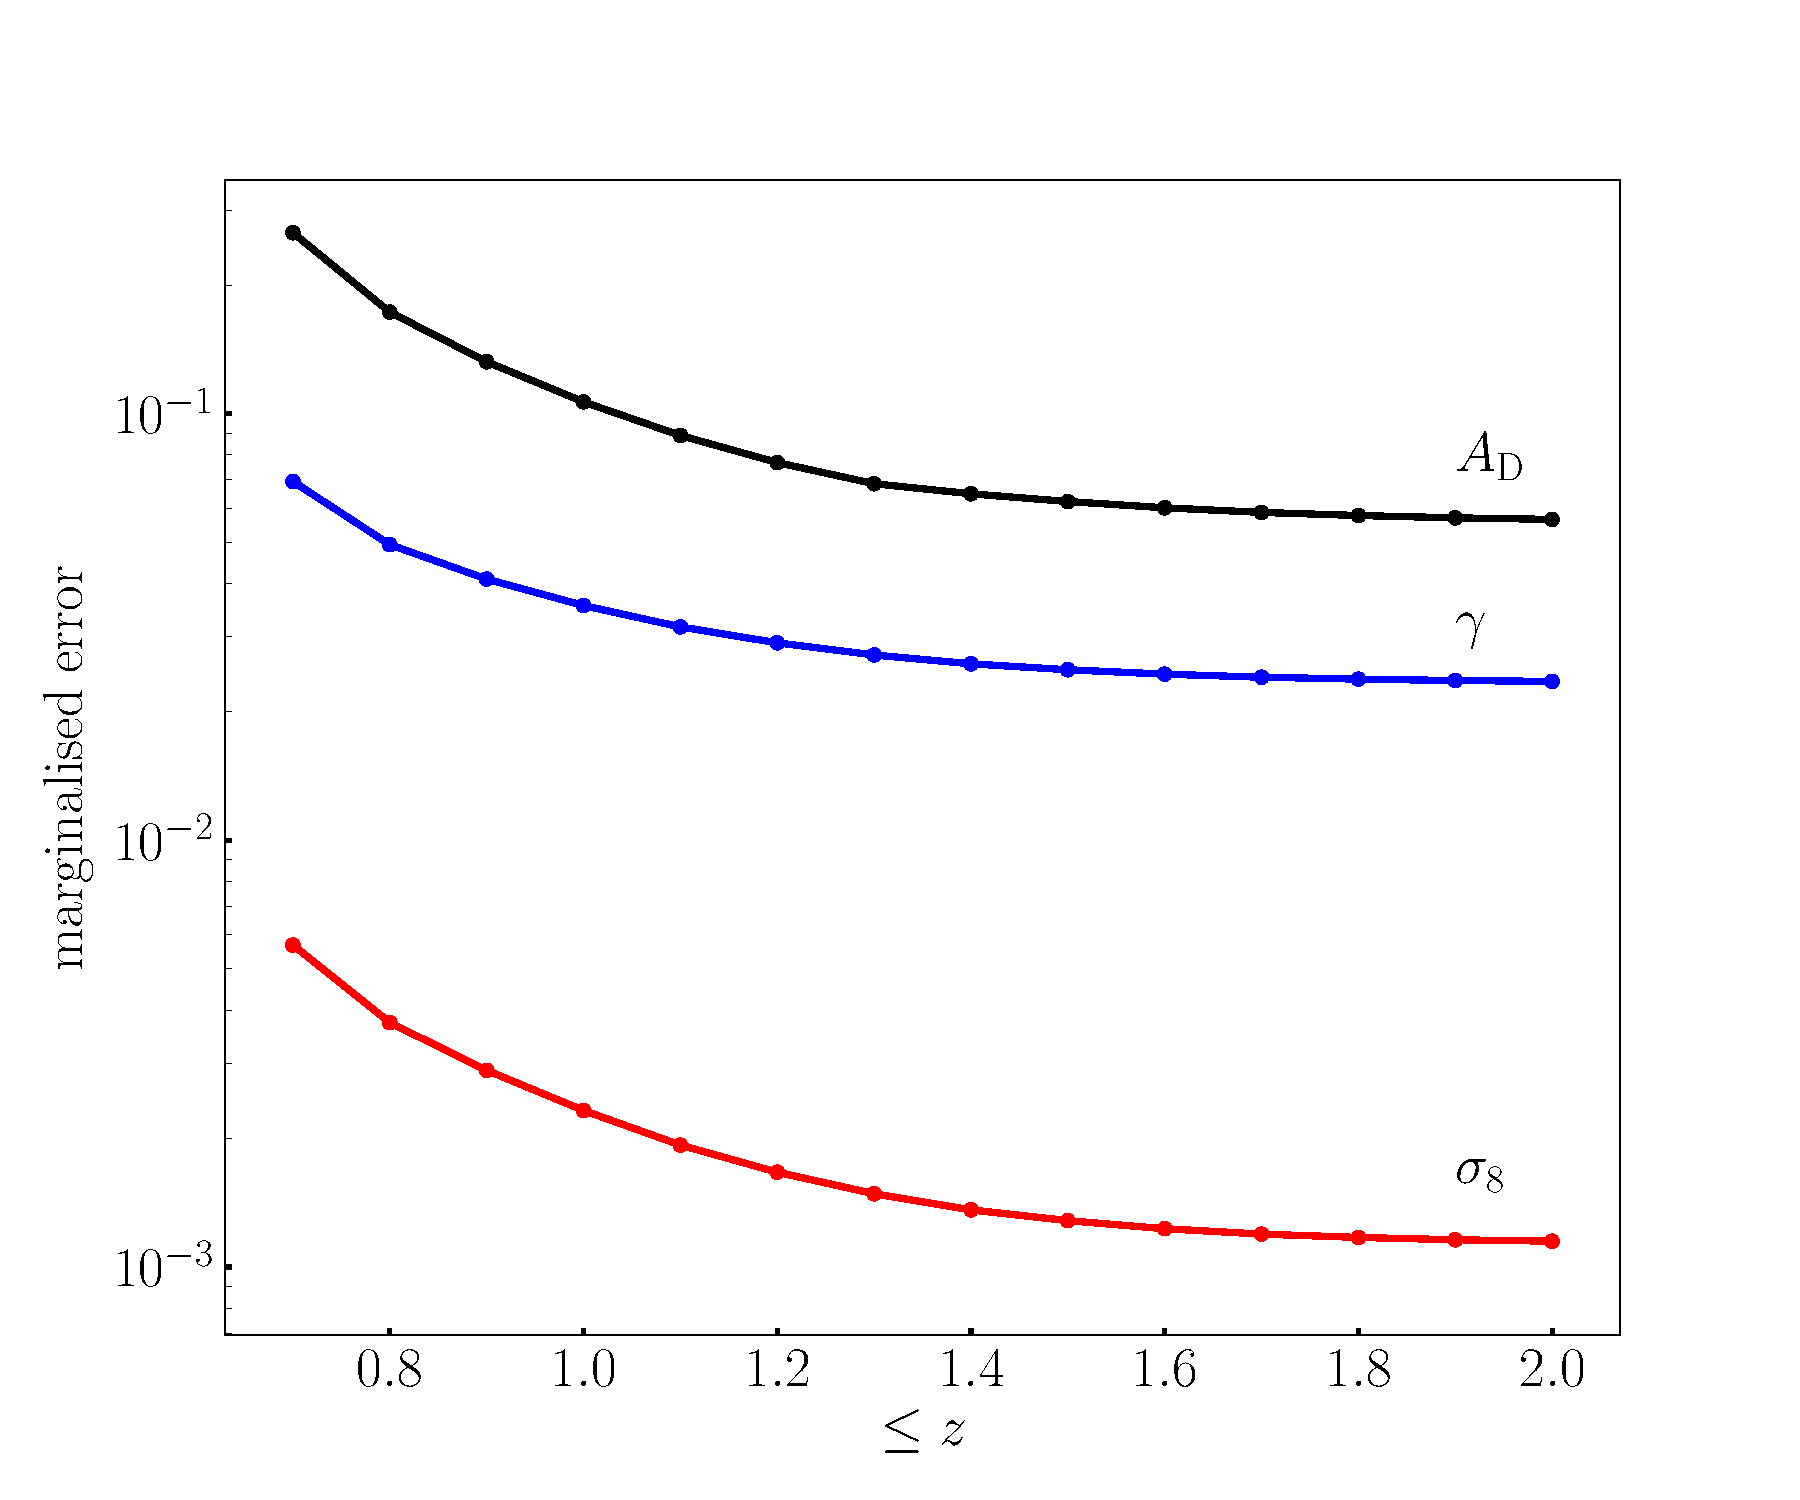
\includegraphics[width=8.0cm]{fig/gamma_sigma8_AD-eps-converted-to}
\caption{Marginal errors (cumulative) on the relativistic contribution, growth index and clustering amplitude, using the full bispectrum.} \label{sig}
\end{figure}
{A full treatment of cosmological constraints would marginalise over the standard cosmological parameters, together with the Alcock-Paczynski parameters and the clustering bias parameters. The constraints obtained would depend almost entirely on the Newtonian galaxy power spectrum and bispectrum (as analysed in \cite{Yankelevich:2018uaz}), given that the relativistic contribution to the power spectrum is below leading order, while in the bispectrum the relativistic SNR is  an order of magnitude smaller than the Newtonian SNR. 

Our focus here is instead on the detectability of the relativistic signal in the bispectrum, {assuming that $P_{g\mathrm{N}}$ and $B_{g\mathrm{N}}$ have been used to constrain the standard parameters.}
We now investigate the effect on this detectability when we include the parameters directly related to redshift-space effects, i.e.,  the growth index $\gamma=\ln f/ \ln\Omega_m$ (with fiducial value 0.545), and the clustering amplitude $\sigma_8$ (with Planck 2018 fiducial).} 
{For forecasts we use the theoretical values of $b_e, \Q$. In a galaxy survey, they would be measured directly from the observed luminosity function, and their measurement uncertainties would need to be marginalised over.}


For the relativistic part of the bispectrum, we introduce a parameter  $A_{\mathrm{D}}$, with fiducial value 1: 
\begin{equation}
B_g=B_{g\mathrm{N}}+A_{\mathrm{D}}\,B_{g\mathrm{D}} \,.
\end{equation}
Then the Fisher matrix for the parameters  $\vartheta_\alpha=(A_{\mathrm{D}},\gamma,\sigma_8)$ is
\begin{equation}
F_{\alpha\beta} = 
\sum_{z,k_a,\,\mu_{1},\,\varphi}\,\frac{1}{{\mathrm{Var}} [{B_{g}}]}
\,\frac{\partial B_{g}}{\partial \vartheta_{(\alpha}}\,\frac{\partial B^*_{g}}{\partial \vartheta_{\beta)}}\,,\label{fm}
\end{equation} 
where the round brackets denote symmetrisation. The cumulative marginal errors $\sigma_\alpha = [(F^{-1})_{\alpha\alpha}]^{1/2}$  are shown in Fig.~\ref{sig}. The fact that $\sigma_{A_{\mathrm{D}}}\lesssim 0.1$  means that the relativistic effects remain detectable when the two additional cosmological parameters are marginalised over.
%

\subsection{Conclusions}


As shown by \cite{Clarkson:2018dwn}, the tree-level galaxy bispectrum in Fourier space has an imaginary part which is a unique signal of the leading-order relativistic corrections in redshift space. These corrections arise from Doppler and other line-of-sight effects on the past lightcone [see \eqref{dg1}, \eqref{dg2}]. In the galaxy bispectrum, the corrections scale as ${\i}\,(\cH/k)P^2$, where $P$ is the linear matter power spectrum [see \eqref{e21}--\eqref{e24}]. By contrast,  at leading order in the galaxy power spectrum, the relativistic correction is real and scales as $(\cH/k)^2P$ -- i.e., it is suppressed by a further factor of  $\cH/k$. 
Only the cross-power spectrum of two different tracers produces an imaginary contribution that scales as ${\i}(\cH/k)P$ \cite{McDonald:2009dh}.
\footnote{See also \cite{Bonvin:2013ogt, Bonvin:2015kuc, Gaztanaga:2015jrs, Irsic:2015nla, Hall:2016bmm,Lepori:2017twd,Bonvin:2018ckp, Lepori:2019cqp} for the corresponding effect in the two-point correlation function, and see \cite{Okoli:2016vmd} for an imaginary {short-scale} contribution from neutrino drag on haloes.}


For a single tracer, the $(\cH/k)^{2}$ relativistic signal in the galaxy {\em power} spectrum is not detectable, even for a cosmic-variance limited survey \cite{Alonso:2015uua}.
The galaxy bispectrum of a single tracer, with its ${\i}\,(\cH/k)$ relativistic contribution, improves the chances of detectability. In addition, the relativistic contribution in the bispectrum couples to short-scale Newtonian terms -- which means that the signal is not confined to very large scales, unlike the case of the power spectrum. We confirmed the expectations of detectability by showing that the signal to noise on the imaginary relativistic part is ${\cal O}(10)$ for a Stage IV $H\alpha$ spectroscopic survey similar to Euclid [see Fig. \ref{fig4}].  We checked that detectability is not compromised by including the uncertainties on two cosmological growth parameters, $\sigma_8$ and $\gamma$ [Fig. \ref{sig}], assuming that other cosmological  and nuisance parameters are determined by the Newtonian power spectrum and bispectrum. 


The relativistic SNR depends on the $k_{\mathrm{max}}(z)$ assumed, because of the coupling of relativistic effects to short-scale Newtonian terms [Fig.~\ref{kmsnr}], and  we made a conservative choice \eqref{kmax}, which includes a redshift dependence to reflect the weakening of nonlinearity at higher $z$. 
Accurate modelling of nonlinear effects would allow us to increase the SNR  
 -- this is not at all specific to the relativistic signal,  but is required for the standard analysis of RSD.

The relativistic SNR also relies  on the largest available scales, but very little signal is lost if $k_{\mathrm{min}}/k_{\mathrm{f}}$ is increased by a factor up  to 5, and even a factor of 10 increase leaves a detectable SNR  [Fig. \ref{kmin}].

By contrast, the SNR depends strongly on accurate modelling of the second-order part of the relativistic correction  [Fig.~\ref{fig4z}]. This includes both the theoretical form \eqref{dg2}, and the
 two astrophysical parameters that do not appear in the Newtonian approximation of the galaxy bispectrum: the evolution bias $b_e$ (measuring the deviation from comoving number conservation) and the magnification bias $\Q$ (which is brought into play by a Doppler correction to standard lensing magnification).  A key feature of our analysis is a physically self-consistent derivation of these quantities from the luminosity function [Fig.~\ref{fig2} and \eqref{q}, \eqref{be}].
We showed that the SNR is very sensitive to these parameters [Fig. \ref{fig1x}], which underlines the need for accurate physical modelling. 

We assumed a Gaussian covariance in our computations, but we used the approximation  of \cite{Chan:2016ehg} to include non-Gaussian corrections. 

Further work should include the window function which we have  neglected.
The imaginary part of the galaxy bispectrum generates a dipole, as shown in \cite{Clarkson:2018dwn}. This suggests a multipole analysis that uses the relativistic dipole in addition to the monopole and quadrupole, {which are unaffected by relativistic effects at leading order.} The
window function can also have an imaginary part \cite{Beutler:2018vpe}, which will need to be corrected for. The dipole from the imaginary part of the bispectrum vanishes in equilateral configurations \cite{Clarkson:2018dwn}, which may help to disentangle the relativistic dipole from that of the window function.

{Our analysis, in common with other works on the Fourier bispectrum, implicitly uses the plane-parallel approximation, since the line-of-sight direction ${\bm{n}}$ is fixed. At the cost of significant complexity, the approximation can be avoided, for example by using a Fourier-Bessel analysis of bispectrum multipoles \cite{Castorina:2017inr}. Further work is needed to address this, but we note that errors from the approximation are mitigated in high redshift surveys such as the one considered here.}

Finally, further work also needs to include the effects of lensing magnification, which are excluded in the standard Fourier analysis, but have been included in the galaxy angular bispectrum \cite{Kehagias:2015tda,DiDio:2015bua, DiDio:2016gpd, DiDio:2018unb} and in a spherical Bessel analysis \cite{Bertacca:2017dzm}. 
%
%
%
%
%
%
%--------------------------------------------
%
%
%
%
%
%
\section{21cm intensity mapping surveys}
%
In this work, we investigate the detectability of the relativistic signal in the bispectrum of various planned 21cm intensity mapping surveys at post-reionisation redshifts. 
The 21cm emission line of neutral hydrogen (HI) is measured without detecting the individual galaxies that contain HI. This results in brightness temperature maps that trace the large-scale structure with exquisite redshift precision. In Section 2 we discuss the leading order relativistic form of the temperature contrast up to second order, and its contribution to the bispectrum. Section 3 describes the signal, modelled using the tree-level bispectrum with the addition of a phenomenological model to account for RSD `fingers-of-god' nonlinearity.
Foreground contamination overwhelms the signal, and cleaning techniques must be applied which lead to a loss of signal in regions of Fourier space, which we take into account. We also discuss the effects of telescope beams and the instrumental noise. Our forecast signal to noise for future surveys is presented in Section 4, and we conclude in Section 5.

\subsection{Relativistic effects in the 21cm IM bispectrum}
%
The HI brightness temperature measured at redshift $z$ in direction $\n$ is related to the observed number of 21cm emitters per redshift per solid angle, $N_{\hi}$, as follows (see~\cite{Hall:2012wd,Alonso:2015uua} for details):
\begin{equation}
T_{\hi}(z,\n)= \mathrm{const.}\, \frac{ N_{\hi}(z,\n)}{d_\mathrm{A}(z,\n)^2}\,,
\label{tobs}
\end{equation}
where $d_\mathrm{A}$ is the angular diameter distance.  

The background HI brightness temperature follows from~\eqref{tobs} as~\cite{Villaescusa-Navarro:2018vsg}
\begin{equation} \label{bart}
\bar{T}_{\hi}(z)= 189h\,\frac{(1+z)H_0}{\cH(z)}\Omega_{\hi}(z)~~\mathrm{mK}.
\end{equation}
Here $h=H_0/(100\,$km/s), $\cH=(\ln a)'$ is the conformal Hubble rate, and $\Omega_{\hi}(z)$ is the comoving HI density in units of the critical density today, which is currently poorly constrained by observations and is modelled by simulations. We use the fit in~\cite{Santos:2017qgq}:
\begin{equation}
\bar{T}_{\hi}(z) = 0.0 56 +0.23\,z -0.024\, z^{2} ~~ \mathrm{mK}. \label{e1.24}
\end{equation}

The temperature fractional perturbation ism
\begin{equation}
\Delta_{\hi}(z,\n) = \frac{T_{\hi}(z,\n) - \bar{T}_{\hi} (z)}{\bar{T}_{\hi} (z)}\,.\label{e1.1_02}
\end{equation}
Using~\eqref{tobs}, this leads to the following perturbative expansion (our convention is $X+X^{\tw}/2$).(A clear and concise derivation of the following expressions for $\Delta$ and $\Delta^{(2)}$ is given in Appendix A of \cite{DiDio:2018zmk}.)
\begin{itemize}
\item 
{\bfseries At first order} \cite{Hall:2012wd}:
\begin{equation} \label{dt1}
\Delta \equiv \Delta^{(1)}_{\hi} = \Delta_\mathrm{N} + \Delta_\mathrm{D}\,,\quad  \Delta_\mathrm{N} = b_1\delta_m - \frac{1}{\cH} \p_r(\v\cdot\n )\,,\quad \Delta_\mathrm{D}=A\,(\v\cdot\n ) \,.
\end{equation}
Here $r$ is the radial comoving distance and $\v=\bm{\nabla}V$ is the peculiar velocity.
$ \Delta_\mathrm{N}$ is the standard density + RSD term, which scales as $\delta_\mathrm{m}$. $\Delta_\mathrm{D}$ is the dominant relativistic correction, scaling as i\,$(\cH/k)\delta_m$ in Fourier space. This Doppler term has coefficient
\begin{equation}
A = b_e - 2 - \frac{\cH'}{\cH^{2}}= -\frac{\ud \ln \left[(1+z) \bar{T}_{\hi} \right]}{\ud \ln (1+z)} \,,
 \label{eq:AcoeffTrel}
\end{equation}
where the evolution bias is~\cite{Fonseca:2015laa},
\begin{equation}
b_e = -\frac{\ud \ln \left[(1+z)^{-1}\cH\, \bar{T}_{\hi} \right]}{\ud \ln (1+z)}\,.
\end{equation}
We omit sub-leading relativistic corrections that scale as $(\cH/k)^2\delta_m$. 
%
%
\item
{\bfseries At second order}
\cite{Maartens:2019yhx} (see also \cite{Umeh:2015gza,DiDio:2015bua,Umeh:2016thy,Clarkson:2018dwn,DiDio:2018zmk}):
\begin{align}
\Delta^{\tw} &\equiv \Delta^{(2)}_{\hi} = \Delta^{\tw}_\mathrm{N} + \Delta^{\tw}_\mathrm{D} \,,\\
\Delta^{\tw}_\mathrm{N}&= b_1\delta_m^{\tw}+b_2 \left(\delta_m \right)^2+ b_{s^2}s^2 + \mathrm{RSD}^{\tw}\,,
\label{d2n} \\
\Delta^{\tw}_\mathrm{D} &= A\, (\v^{(2)}\!\!\cdot\n)+2\left[ b_{1} (A+f) + \frac{b_1'}{\cH}\right]\,(\v\cdot\n)\,\delta_m +\frac{1}{\cH}\left( 8 - 4 A-3 \Omega_m \right)(\v\cdot\n)\,\partial_r(\v \cdot \n)
\nonumber\\ \label{e1.2}
&+\frac{2}{\cH^2}\left[(\v\cdot\n) \,\partial_r^2\Phi-\Phi\, \partial_r^2 (\v\cdot\n) \right]
 -\frac{2}{\cH}\,\partial_r (\v\cdot\v)+2 \frac{{b_{1}}}{\cH}\,\Phi\, \partial_r\delta_m \,.
\end{align}
In~\eqref{d2n}, $b_{s^2}s^2$ is the tidal bias contribution and RSD$^{\tw}$ is the standard second-order RSD contribution (see \cite{Maartens:2019yhx} for details). The bias parameters are computed via a halo model and are shown in Figure \ref{fig:detectfigbiasparam}, together with the evolution bias.
In~\eqref{e1.2}, we see the Doppler terms and the line-of-sight gradients that make up the dominant relativistic contribution.
 $\Phi$ is the gravitational potential and $\Omega_m =\Omega_{m 0}(1+z)H_0^2/\cH^2$. We  neglect sub-dominant relativistic effects in $\Delta^{\tw}$ that scale as  $(\cH/k)^2(\delta_m)^2$. 
%
\begin{figure}[ht]
\centering
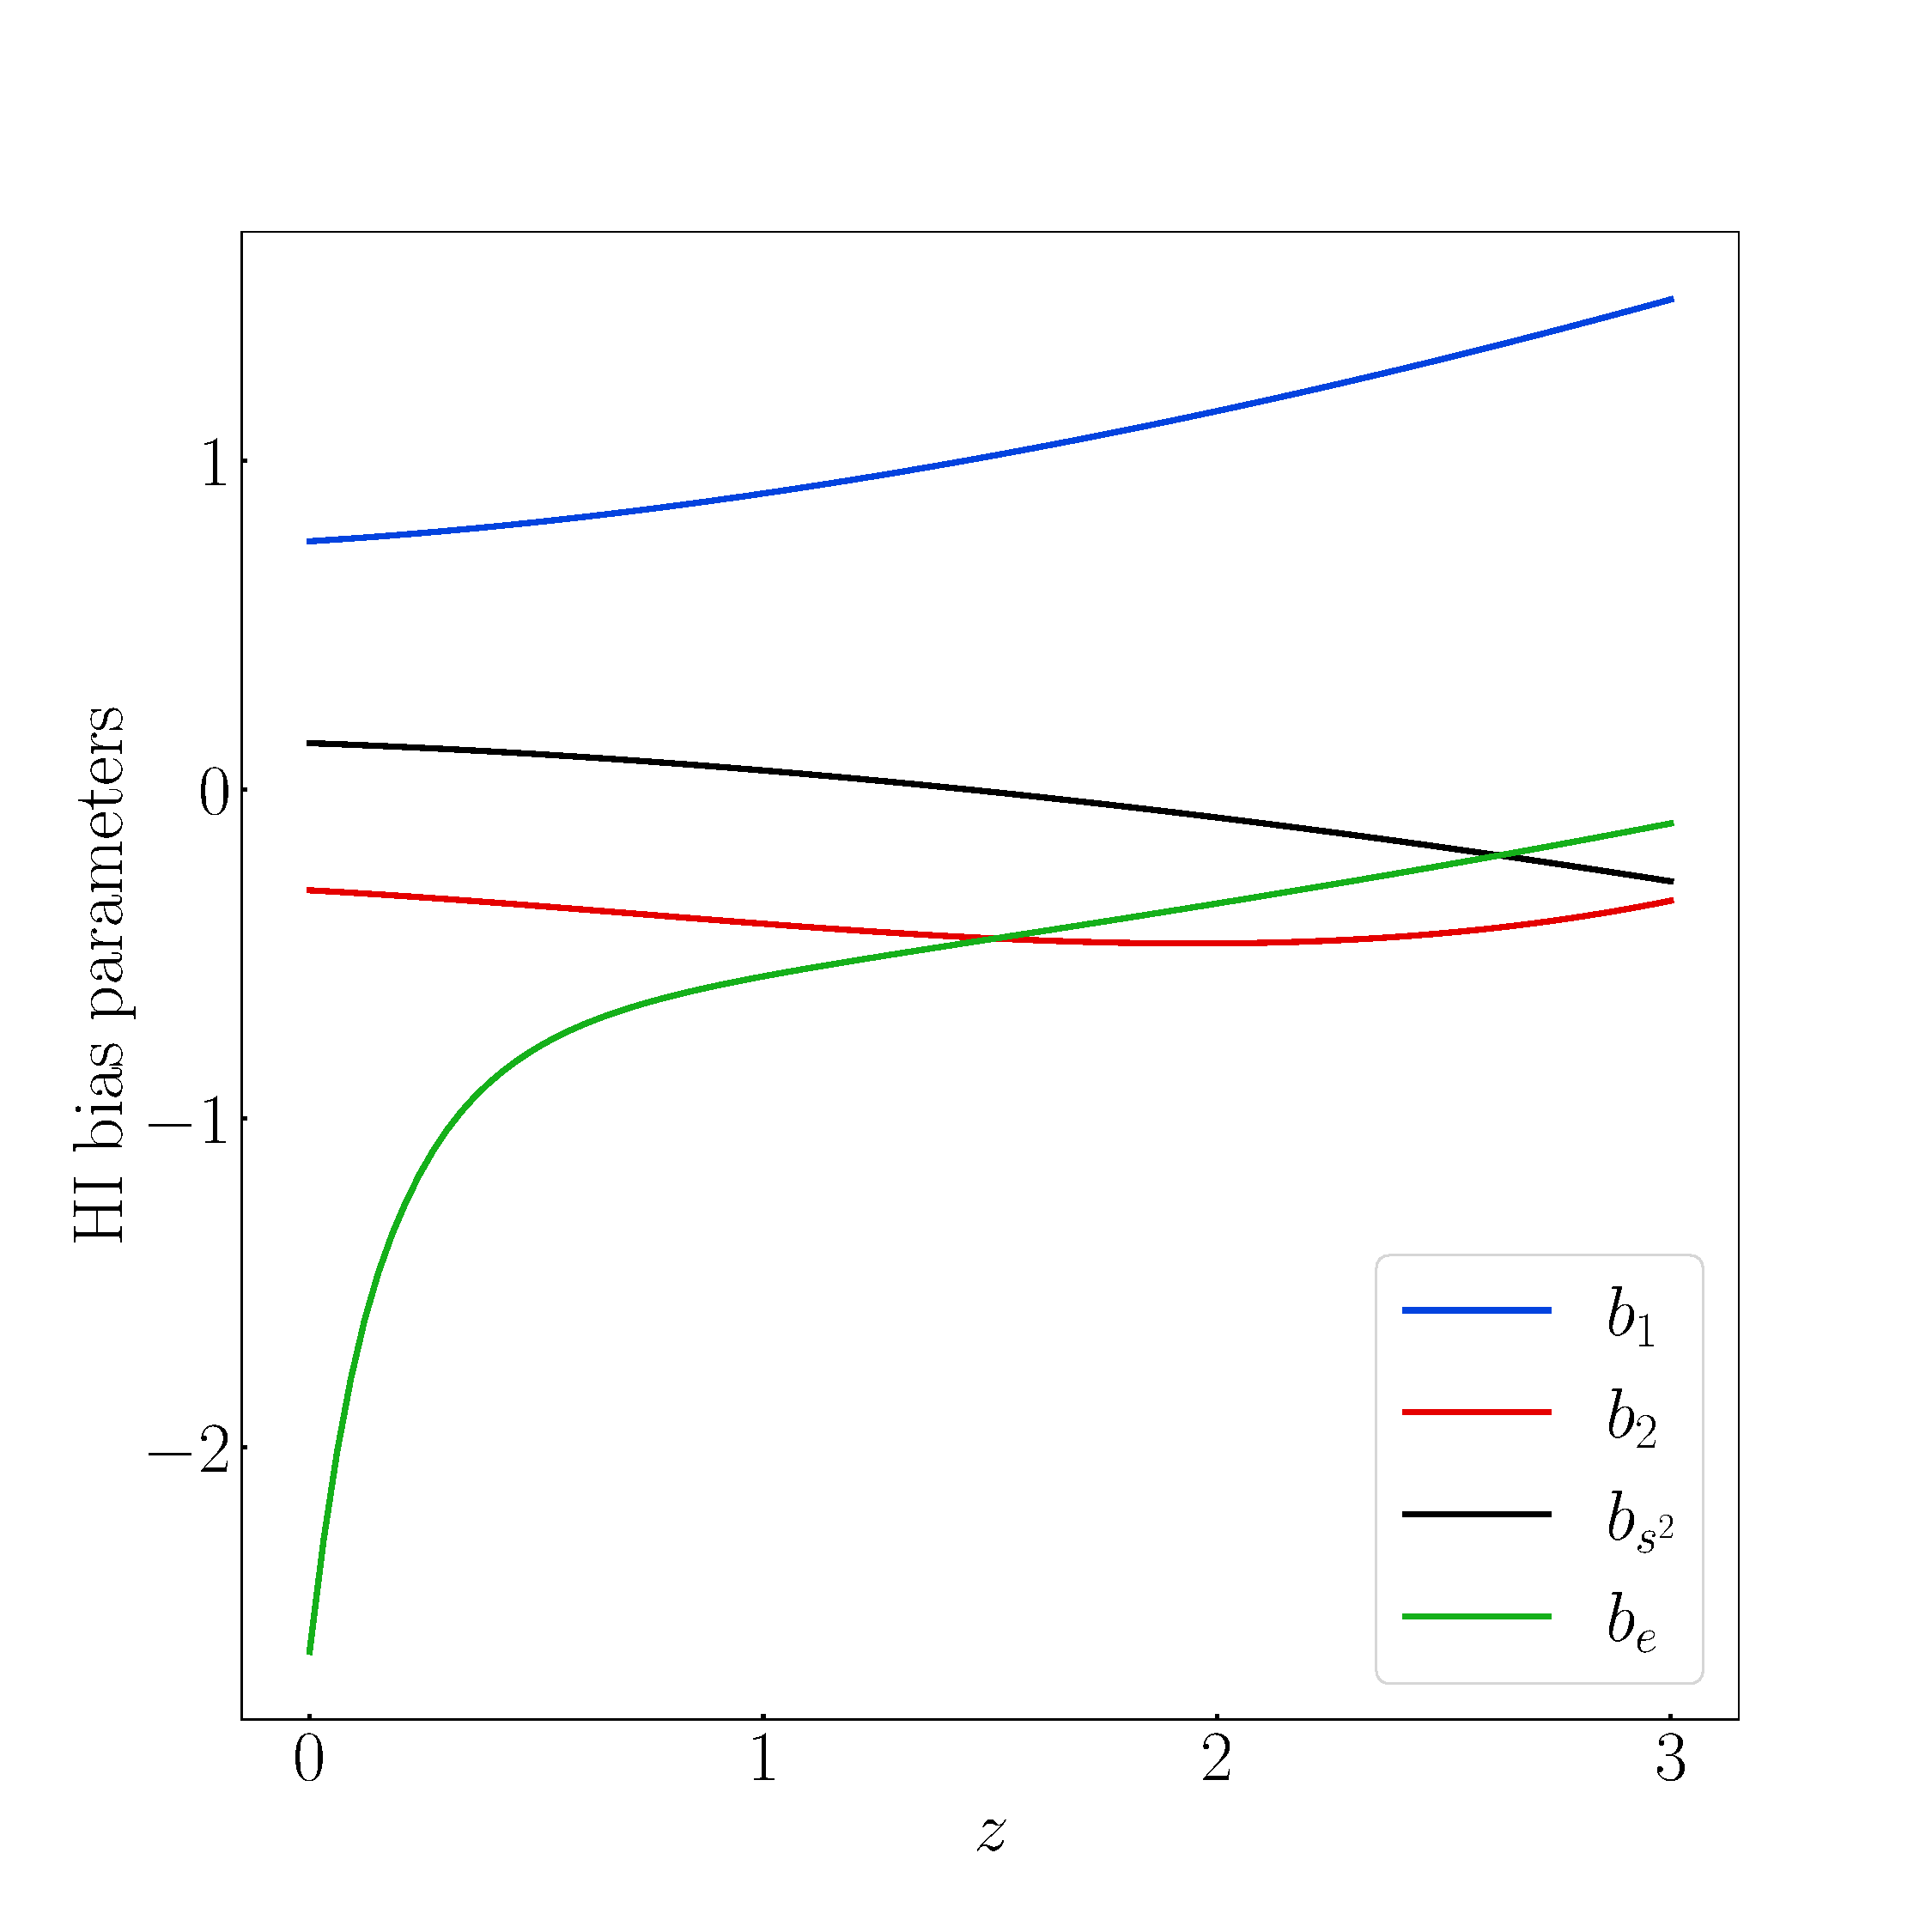
\includegraphics[width=.49\textwidth]{fig/HIBias.pdf}
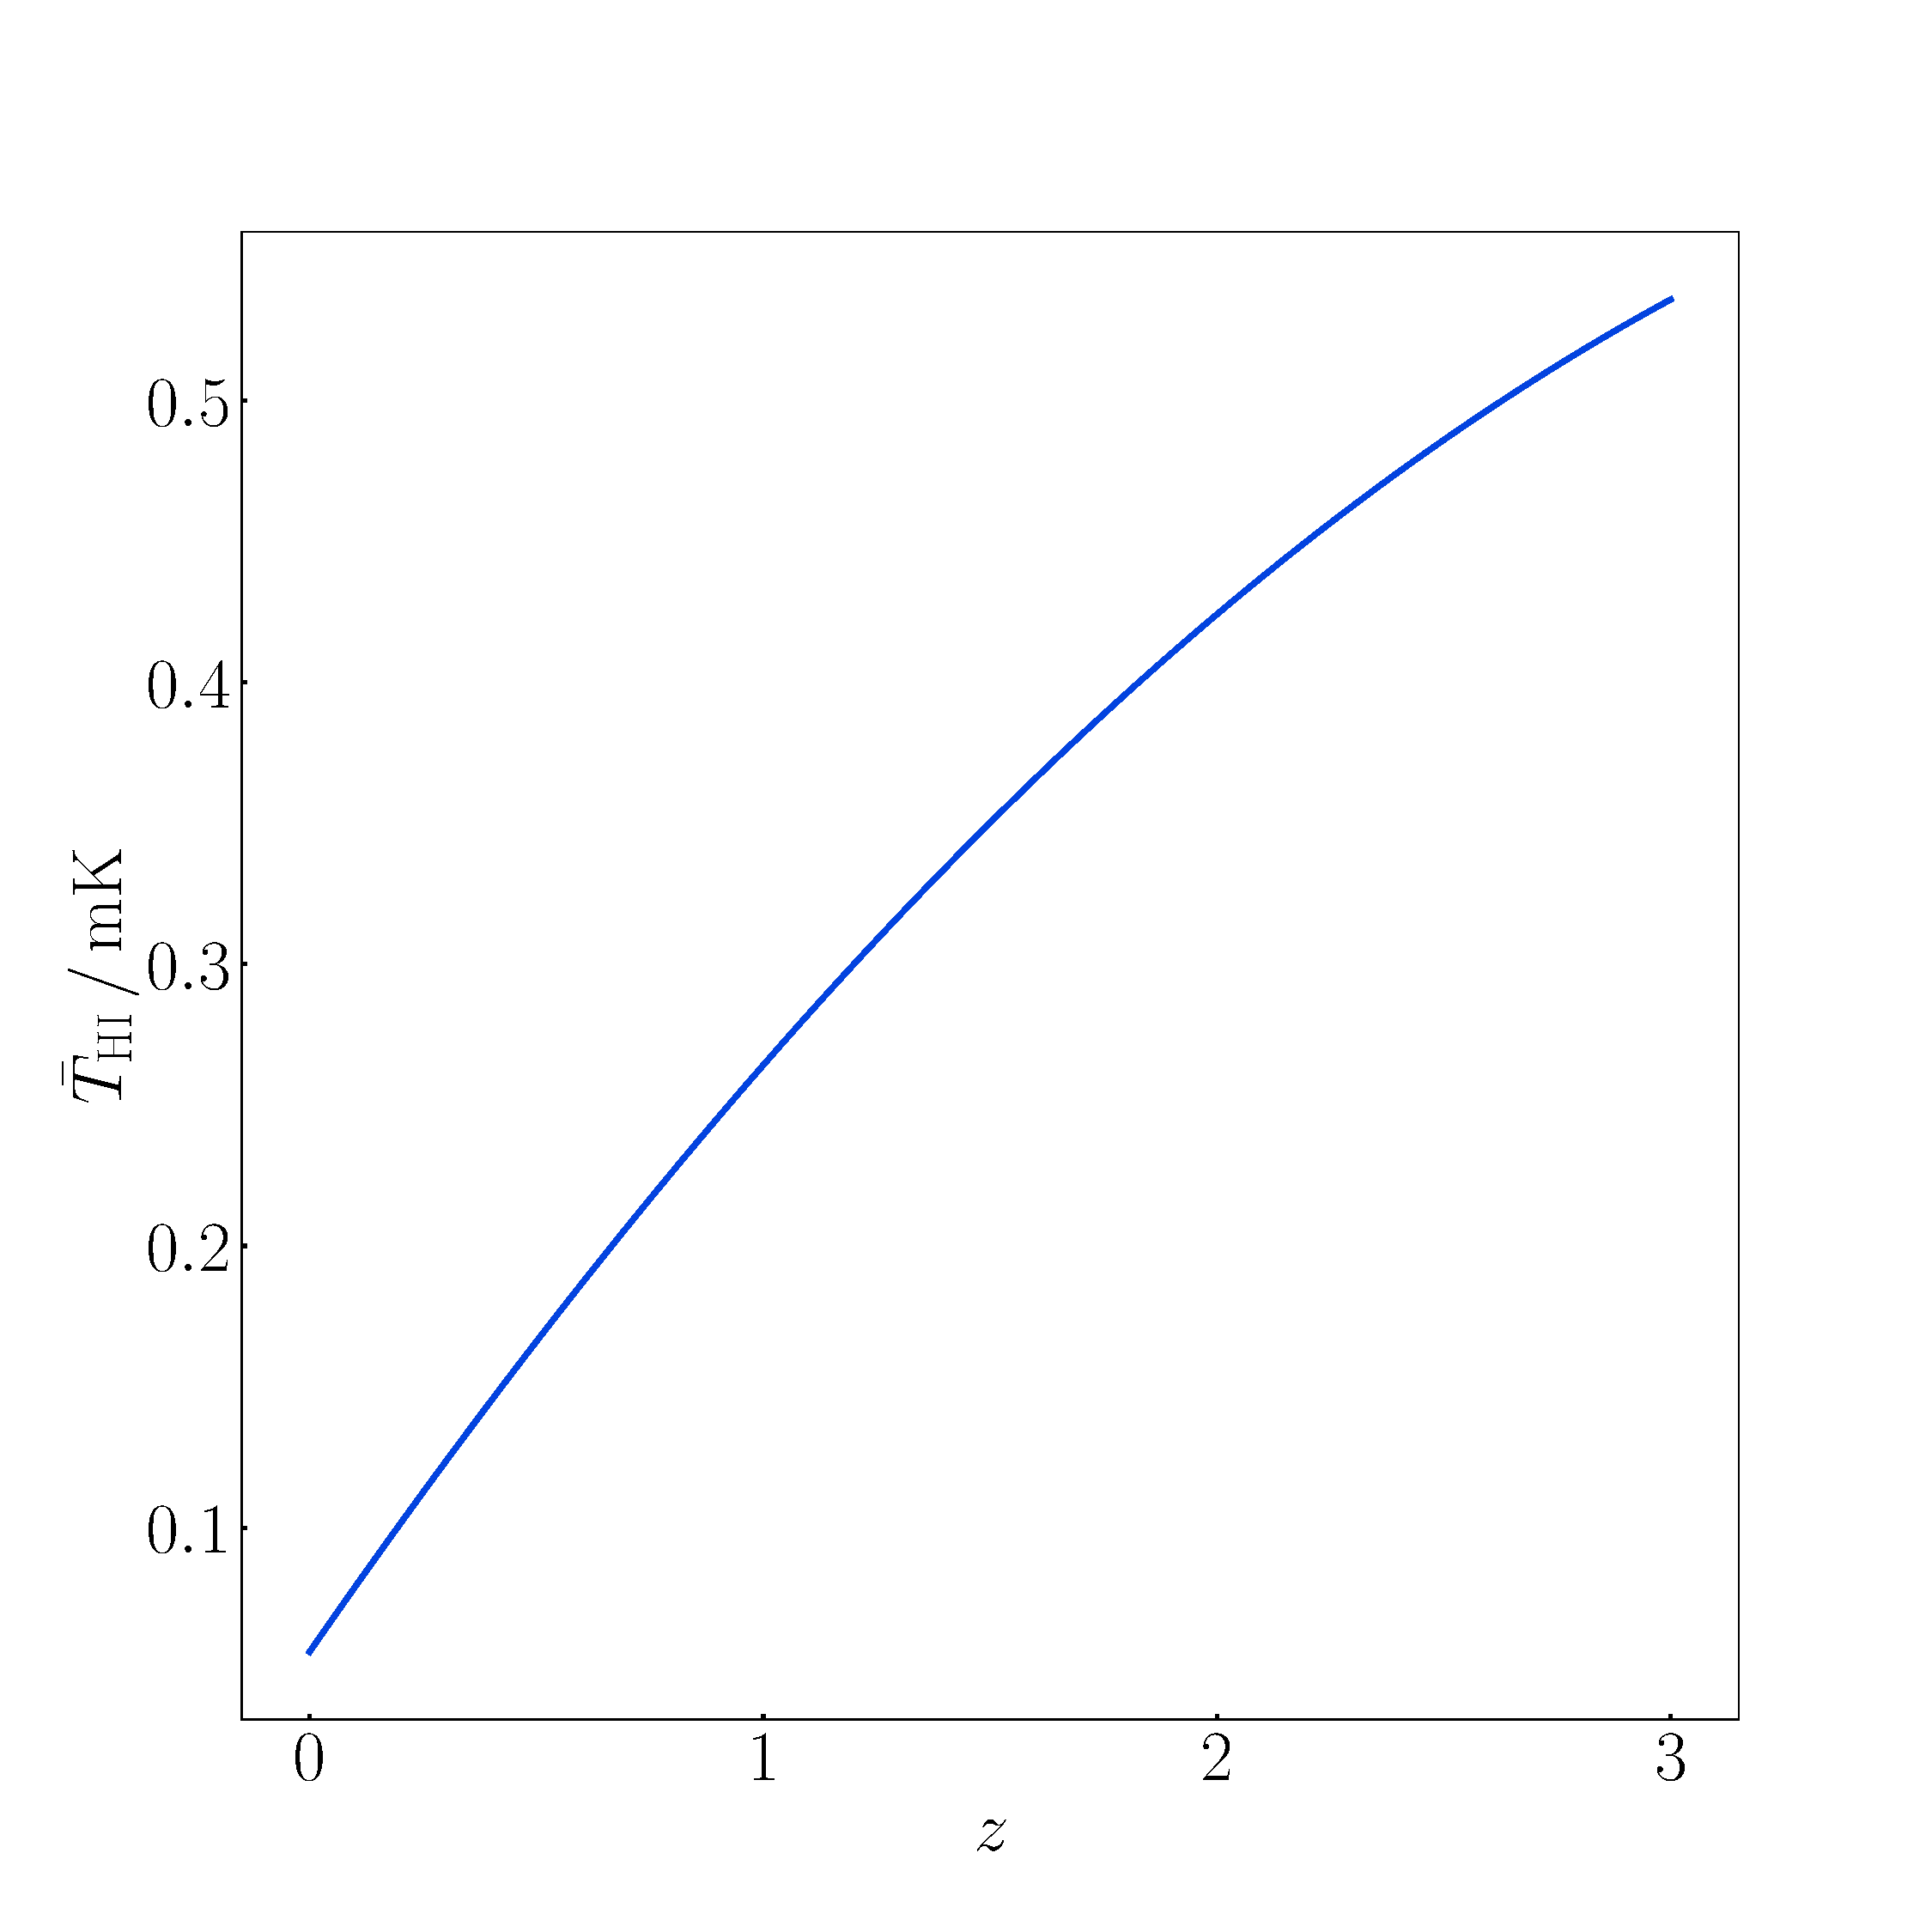
\includegraphics[width=.49\textwidth]{fig/THI.pdf}
\caption{HI clustering and evolution bias parameters (left) and background temperature (right).}\label{fig:detectfigbiasparam}
\end{figure}
%
%
\item {\bfseries Lensing contribution:}\\
At first order, there is no lensing contribution to $\Delta$ \cite{Hall:2012wd}. The general case of galaxy number density contrast contains a lensing  contribution $2({\cal Q}-1)\kappa$ to $\Delta_g$, where $\kappa$ is the convergence \cite{Challinor:2011bk}.  For HI emitters in intensity mapping, the magnification bias satisfies
\begin{equation}
{\Q} \equiv -\frac{\p \ln \bar{N}_{\hi}}{\p \ln L}\bigg|_\mathrm{c} = 1\,, \label{magb}
\end{equation}
where c indicates evaluation at the luminosity cut. 

At second order, \eqref{tobs} shows that there is also no contribution to $\Delta^{\tw}$ from lensing convergence~\cite{DiDio:2015bua,Jalivand:2018vfz}. We can recover this result from the full general expression for second-order number density contrast~\cite{Bertacca:2014dra, Bertacca:2014wga, Yoo:2014sfa, DiDio:2014lka, Bertacca:2014hwa}, by imposing \eqref{magb} together with the conditions~\cite{DiDio:2015bua}
\begin{equation} \label{magb2}
\frac{\p^2 \ln \bar{N}_{\hi}}{\p (\ln L)^2}\bigg|_\mathrm{c} = 0\,, \quad  \frac{\p b_1}{\p \ln L}\bigg|_\mathrm{c}=0\,.
\end{equation}

There remains however a lensing deflection contribution $\nabla_{\perp a}\Delta\,\nabla_\perp^a\phi$ to  $\Delta^{\tw}$,  where $\nabla_{\perp a}$ is a screen-space gradient and $\phi$ is the lensing potential~\cite{Umeh:2015gza,DiDio:2015bua,Jalivand:2018vfz}. In the bispectrum the contribution of this term is negligible for equal-redshift correlations~\cite{DiDio:2015bua,Durrer:2020orn}. Since we only consider the bispectrum at equal redshifts, we can safely neglect this term. 
\end{itemize}
\vspace{0.2cm}
%
In Fourier space, the HI bispectrum at tree level is defined by,
\begin{equation}
\left\langle \Delta(z,\ka)\Delta(z,\kb)\Delta^{(2)}(z,\kc) \right\rangle + \text{2 cp}=2 (2\pi)^3 B_{\hi}(z, \ka, \kb, \kc) \delta^\mathrm{Dirac}\left(\ka + \kb + \kc\right)\,, \label{e1.3}
\end{equation}
where cp denotes cyclic permutation. It follows that, 
\begin{equation}
B_{\hi}(z, \ka,\kb,\kc) = \mathcal{K}^{(1)}(z, \ka)\mathcal{K}^{(1)}(z, \kb)\mathcal{K}^{(2)}(z, \ka,\kb,\kc)P_\mathrm{m} (z, k_{1})P_\mathrm{m}(z, k_{2}) + \text{2 cp}\,, \label{e1.5}
\end{equation} 
where $P_\mathrm{m}$ is the linear matter power spectrum (computed using CLASS~\cite{Blas:2011rf}).  From now on, we often drop the $z$ dependence for brevity.  
The bispectrum kernels are as follows:
\begin{itemize}
\item
{\bfseries Standard (Newtonian) kernels:}
\begin{align}
\mathcal{K}^{(1)}_\mathrm{N}(\ka) &= b_1 + f\mu_{a}^{2}\,,  \label{e1.7} \\ 
\mathcal{K}^{(2)}_\mathrm{N}(\ka,\kb,\kc) &= b_1 F_2(\ka,\kb) + b_2 + f\mu_{3}^{2} G_2(\ka,\kb) + f \cZ_2(\ka,\kb)
+ b_{s^{2}}S_{2}(\ka,\kb)\,, \label{e1.8}
\end{align}
where $f$ is the linear matter growth rate, $\mu_a=\hat{\k}_a\cdot\n$ and the standard $F_2,G_2,\cZ_2,S_2$ kernels are given in \cite{Maartens:2019yhx}.

\item
{\bfseries Leading-order relativistic kernels:} 
\begin{align}
\mathcal{K}^{(1)}_{\mathrm{D}}(\ka) &= \i \cH f A\,\frac{\mu_{a}}{k_{a}}\,, \label{e1.9} \\
\mathcal{K}^{(2)}_{\mathrm{D}}(\ka,\kb,\kc) &= \i \cH f \left\{
A\,\frac{\mu_{3}}{k_{3}} G_{2}(\ka,\kb)
+{\left[ b_1\left( A+f \right) + \frac{b_1'}{\cH} \right]}\left(\frac{\mu_{1}}{k_{1}} + \frac{\mu_{2}}{k_{2}}\right) \right.
\nonumber \\
& \left. -\frac{3}{2}\Omega_m \left(\mu_{1}^{3} \frac{k_{1}}{k_{2}^{2}} + \mu_{2}^{3}\frac{k_{2}}{k_{1}^{2}}\right)
+ \left[\frac{3}{2}\Omega_m \left(1+f \right)+2f\left(A-2\right) \right] \mu_{1}\mu_{2}\left(\frac{\mu_{1}}{k_{2}}+\frac{\mu_{2}}{k_{1}}\right) \right.
\nonumber \\
& \left. + 2 f \,  {\hat{\bm{k}}_{1} \cdot \hat{\bm{k}}_2}\left(\frac{\mu_{1}}{k_{1}} + \frac{\mu_{2}}{k_{2}}\right) 
-\frac{3\Omega_m b_1}{2f} \left(\mu_{1}\frac{k_{1}}{k_{2}^{2}} + \mu_{2}\frac{k_{2}}{k_{1}^{2}}\right)\!  \right\}\,,\label{e1.10}
\end{align}
where $A$ is given by~\eqref{eq:AcoeffTrel}. These follow from~\eqref{dt1} and \eqref{e1.2}, and {agree with~\cite{Maartens:2019yhx} when we impose~\eqref{eq:AcoeffTrel}, \eqref{magb} and~\eqref{magb2}}.
\item
{\bfseries Complex bispectrum:}\\
From~\eqref{e1.7}--\eqref{e1.10} we see that
$B_{\hi}$ is complex: {the imaginary part is given purely by local relativistic corrections, while at leading order, i.e. neglecting relativistic terms of $\ord(\cH^2/k^2)$, the real part is given purely by the standard Newtonian bispectrum:}
\begin{align}
\mathrm{Re}\left( B_{\hi} \right) &= B_\mathrm{N} = \mathcal{K}^{(1)}_\mathrm{N}(\ka) \mathcal{K}^{(1)}_\mathrm{N}(\kb) \mathcal{K}^{(2)}_\mathrm{N}(\ka,\kb,\kc)P_\mathrm{m} (k_{1}) P_\mathrm{m} (k_{2}) + \text{2 cp}, \label{e1.14}\\
\i \mathrm{Im} \left(B_{\hi}\right) &= B_\mathrm{D} = \left\{ \left[ \mathcal{K}^{(1)}_{\mathrm{N}}(\ka)\mathcal{K}^{(1)}_{\mathrm{D}}(\kb) + \mathcal{K}^{(1)}_{\mathrm{D}}(\ka)\mathcal{K}^{(1)}_{\mathrm{N}}(\kb)\right]\mathcal{K}^{(2)}_{\mathrm{N}}(\ka,\kb,\kc) \right. \label{e1.15}\\ \nonumber 
&\left. ~~~~~~~~~~~~~ +\mathcal{K}^{(1)}_{\mathrm{N}}(\ka)\mathcal{K}^{(1)}_{\mathrm{N}}(\kb)\mathcal{K}^{(2)}_{\mathrm{D}}(\ka,\kb,\kc)\right\}P_\mathrm{m} (k_{1})P_\mathrm{m} (k_{2})+\text{2 cp}.
\end{align}
It is apparent that {$B_\mathrm{N} \sim P_\mathrm{m} ^2$ while $B_\mathrm{D} \sim \i (\cH/k) P_\mathrm{m} ^2$.}
Equation~\eqref{e1.15} makes explicit the coupling of relativistic  and Newtonian terms in the bispectrum.
\end{itemize}

\subsubsection{HI bias parameters} 
We follow~\cite{Umeh:2015gza} to compute $b_1$ and $b_2$ from a halo-model approach,
\begin{align}
b_1 &= 1 + \left\langle \frac{2 p +\left(q\nu - 1\right)\left[1+(q\nu)^{p}\right]}{\delta_\mathrm{cr}\left[1+(q\nu)^{p}\right]} \right\rangle _\mathrm{\!\!\! m}  \!\!, \label{e1.16} \\
b_2 &= \frac{8}{21}\left(b_{1}-1\right) + \left \langle \frac{2 p \left(2p+2\nu q-1\right)+ q\nu\left(q\nu-3\right)\left[1+(q\nu)^{p}\right]}{\delta_\mathrm{cr}^{2}\left[1+(q\nu)^{p}\right]}  \right \rangle _\mathrm{\!\!\! m}  \!\!, \label{e1.17}
\end{align}
where the parameters $p$, $q$ and $\nu$ are related to the Sheth-Tormen distribution function (see~\cite{Sheth:1999su, Sheth:2001dp, Sheth:1999mn} for more details), and $\delta_\mathrm{cr}$ is the critical density at which halos collapse spherically~\cite{Kitayama:1996ne}, 
\begin{equation}
\delta_\mathrm{cr}(z) = \frac{3(12\pi)^{2/3}}{20} \left[1+0.0123\log{\Omega_m (z)}\right] \,. \label{e1.20}\,.
\end{equation}
The mass average is defined by 
\begin{equation}
\left\langle X_{h}(z,\bm{x}) \right\rangle _\mathrm{m}  = \frac{\int_{M_{-}}^{M_{+}} \ud M\,X_{h}(z,\bm{x},M)\,M_{\hi}(M)\,n_{h}(z,\bm{x},M)}{\int_{M_{-}}^{M_{+}} \ud M\,M_{\hi}(M)\,n_{h}(z,\bm{x},M)} \, , \label{e1.18}
\end{equation}
where $M$ is the mass of halos that can host HI gas, and $M_{\pm}$ are the lower and upper mass limits, which are related to the circular velocities  of the galaxies~\citep{Bull:2014rha}. $n_{h}$ is the halo mass function~\citep{Sheth:1999su, Sheth:2001dp,Tellarini:2015faa}, and $M_{\hi}$ is the HI mass function, which is assumed to follow a power law~\citep{Santos:2015gra},
\begin{equation}
M_{\hi}(M) \propto M^{0.6} \,. \label{e1.19}
\end{equation}
Figure~\ref{fig1} shows the numerical results from~\eqref{e1.16} and~\eqref{e1.17}. Fitting formulas for the bias parameters are
\begin{align}
b_1(z) &=  0.754 + 0.0877z + 0.0607z^2 - 0.00274z^3\,, \label{e1.27} \\
b_2(z) &=  -0.308 - 0.0724z - 0.0534z^2 + 0.0247z^3\,. \label{e1.28}
\end{align}
Assuming that halo formation is a local process in Lagrangian space and that there is no initial tidal bias, the tidal bias is~\cite{Tellarini:2015faa},
\begin{equation}
b_{s^{2}} = \frac{4}{7}\left(1-b_{1}\right)\,.\label{e1.21}
\end{equation} 
%


\subsection{Effects of foregrounds}
%
Foreground contamination is the major systematic confronting 21cm intensity mapping. 
Cleaning techniques are very efficient at recovering the cosmological signal in regions of $(k_\|,k_\perp)$ space (see e.g.~\cite{Pober:2013jna, Bull:2014rha, Alonso:2014dhk, Pober:2014lva, Wolz:2015sqa, Santos:2015gra, Shaw:2014khi, Obuljen:2017jiy, Ansari:2018ury, Witzemann:2018cdx, Bacon:2018dui, Asorey:2020mxs, Cunnington:2020mnn}). A realistic model of bispectrum measurements should include modelling of foreground removal. However, our focus is on the relativistic signal in the bispectrum and so we take a simpler approach -- by excising the regions of $(k_\|,k_\perp)$ space where foreground cleaning does not recover the signal efficiently.

HI intensity mapping surveys are planned for next-generation radio dish arrays, including MeerKAT\footnote{www.sarao.ac.za/science/meerkat/}, SKA1-MID\footnote{{www.skatelescope.org/}}, and HIRAX\footnote{hirax.ukzn.ac.za/}. We will also consider surveys with
PUMA\footnote{{www.puma.bnl.gov/}} in its initial phase (Petite) (note that PUMA is currently still a proposal).

Intensity mapping surveys can be done in 2 survey modes:
\begin{itemize}
\item Single-dish (SD) mode: auto-correlation signals from single dishes are added.
\item Interferometer (IF) mode: cross-correlation signals from array elements are combined. 
\end{itemize}  
In both SD- and IF-mode surveys, foreground cleaning effectively removes large-scale radial modes because of the smoothness in freqency of the main foreground emissions. In order to model the effects of foreground cleaning, we remove radial modes $k_\| \equiv \mu k$ that are smaller than a critical scale $k_{\| \fg}$~\cite{Karagiannis:2018jdt}.
We impose this via an exponential damping factor~\cite{Bull:2014rha},
\begin{equation}\label{eq:expdampfact}
D_{\fg}(k,\mu) = 1 - \exp\left[-\left(\frac{\mu k}{k_{\| \fg}}\right)^2\right]\qquad \mbox{for SD and IF survey modes.}
\end{equation}
Then, 
\begin{align}
P_{\hi}(k,\mu,z)  &~\to~ D_{\fg} (k,\mu)\,P_{\hi}(k,\mu,z) \,,\\
B_{\hi}(k_a,\mu_a,z) & ~\to~ D_{\fg} (k_1,\mu_1)\,D_{\fg} (k_2,\mu_2)\,D_{\fg} (k_3,\mu_3)\,B_{\hi}(k_a,\mu_a,z)\,.
\end{align}
The value of $k_{\| \fg}$ can be reduced by techniques which reconstruct long modes from the information in measured short modes. This technique has been applied to HI intensity mapping by~\cite{Zhu:2016esh,Modi:2019hnu}. Taking into account reconstruction, we choose,
\begin{equation} \label{kfgpar}
k_{\| \fg} = 0.01 \,h\,\mathrm{Mpc}^{-1},
\end{equation}
but we will also consider an optimistic case, k$_{\| \fg} = 0.005 \,h\,\mathrm{Mpc}^{-1}$, that anticipates further developments of the reconstruction technique.

IF-mode surveys lose additional signal due to the fact that interferometers are chromatic, i.e. a fixed physical baseline length probes different angular scales at different frequencies. This causes smooth foregrounds to leak into high-$k_{\perp}$ modes~\cite{Obuljen:2017jiy,Alonso:2017dgh,Ansari:2018ury}. The signal loss may be accounted for by excluding
the region known as the foreground wedge~\cite{Pober:2014lva, Pober:2013jna}: 
\begin{equation} \label{e2.19}
\left|k_{\parallel}\right| > k_\mathrm{wedge}(z)\,k_{\perp} \qquad \mbox{for IF survey mode,}
\end{equation} 
where $k_\perp=\sqrt{1-\mu^2}\,k$ and $k_\mathrm{wedge}$ is modelled as,
\begin{equation}
k_\mathrm{wedge}(z) = r(z) \cH(z) \sin{\left[0.61N_{\mathrm{w}}\,{\theta_\mathrm{b}(z)}\right]} \,. \label{e2.20} 
\end{equation}
The beam (defining the IF field of view) is given for a dish array by,
\begin{equation}\label{thetab}
\theta_\mathrm{b}(z) = 1.22 \,\frac{\lambda(z)}{D_\mathrm{d}}\,,
\end{equation}
where $\lambda(z)=\lambda_{21}(1+z)$ and $D_\mathrm{d}$ is the dish diameter.
$N_{\mathrm{w}}$ is the number of primary beams away from the beam centre that contaminate the signal. The wedge effect is a technical problem that can be mitigated (and  in principle removed) by calibration of baselines~\cite{Ghosh:2017woo}.
Following~\cite{Karagiannis:2019jjx}, we take
\begin{equation}
N_{\mathrm{w}}= 0, 1, 3, 
\end{equation}
where 0 is the most optimistic possibility (wedge removed by calibration) and 3 is a pessimistic case. 
%
\subsection{Maximum and minimum scales probed}
%
The nonlinearity limit $k\leq k_\mathrm{max}(z)$ given in~\eqref{kmax}, defines a minimum wavelength $2\pi/ k_\mathrm{max}(z)$ that is independent of surveys and is determined purely by dark matter clustering. It applies to both SD- and IF-mode surveys.
However, in the case of IF-mode surveys, there is also a lower limit on angular scales, i.e. an upper limit on transverse wavenumbers, via $k_\perp=2\pi/(r\theta)$. This arises because the maximum baseline $D_\mathrm{max}$ determines the  angular resolution  and the upper limit can be roughly estimated by a cut-off~\cite{Bull:2014rha,Alonso:2017dgh,Karagiannis:2019jjx,Durrer:2020orn},
\begin{equation} \label{kifmax}
k_{\perp \mathrm{max}}^\mathrm{IF}(z) \approx \frac{2\pi D_\mathrm{max}}{r(z)\,\lambda(z)}\,.
\end{equation}
In our computations, we do not use this cut-off since it is effectively imposed by the baseline density factor (see Section~\ref{ssec:inoise}).
\begin{figure}[ht]
\centering
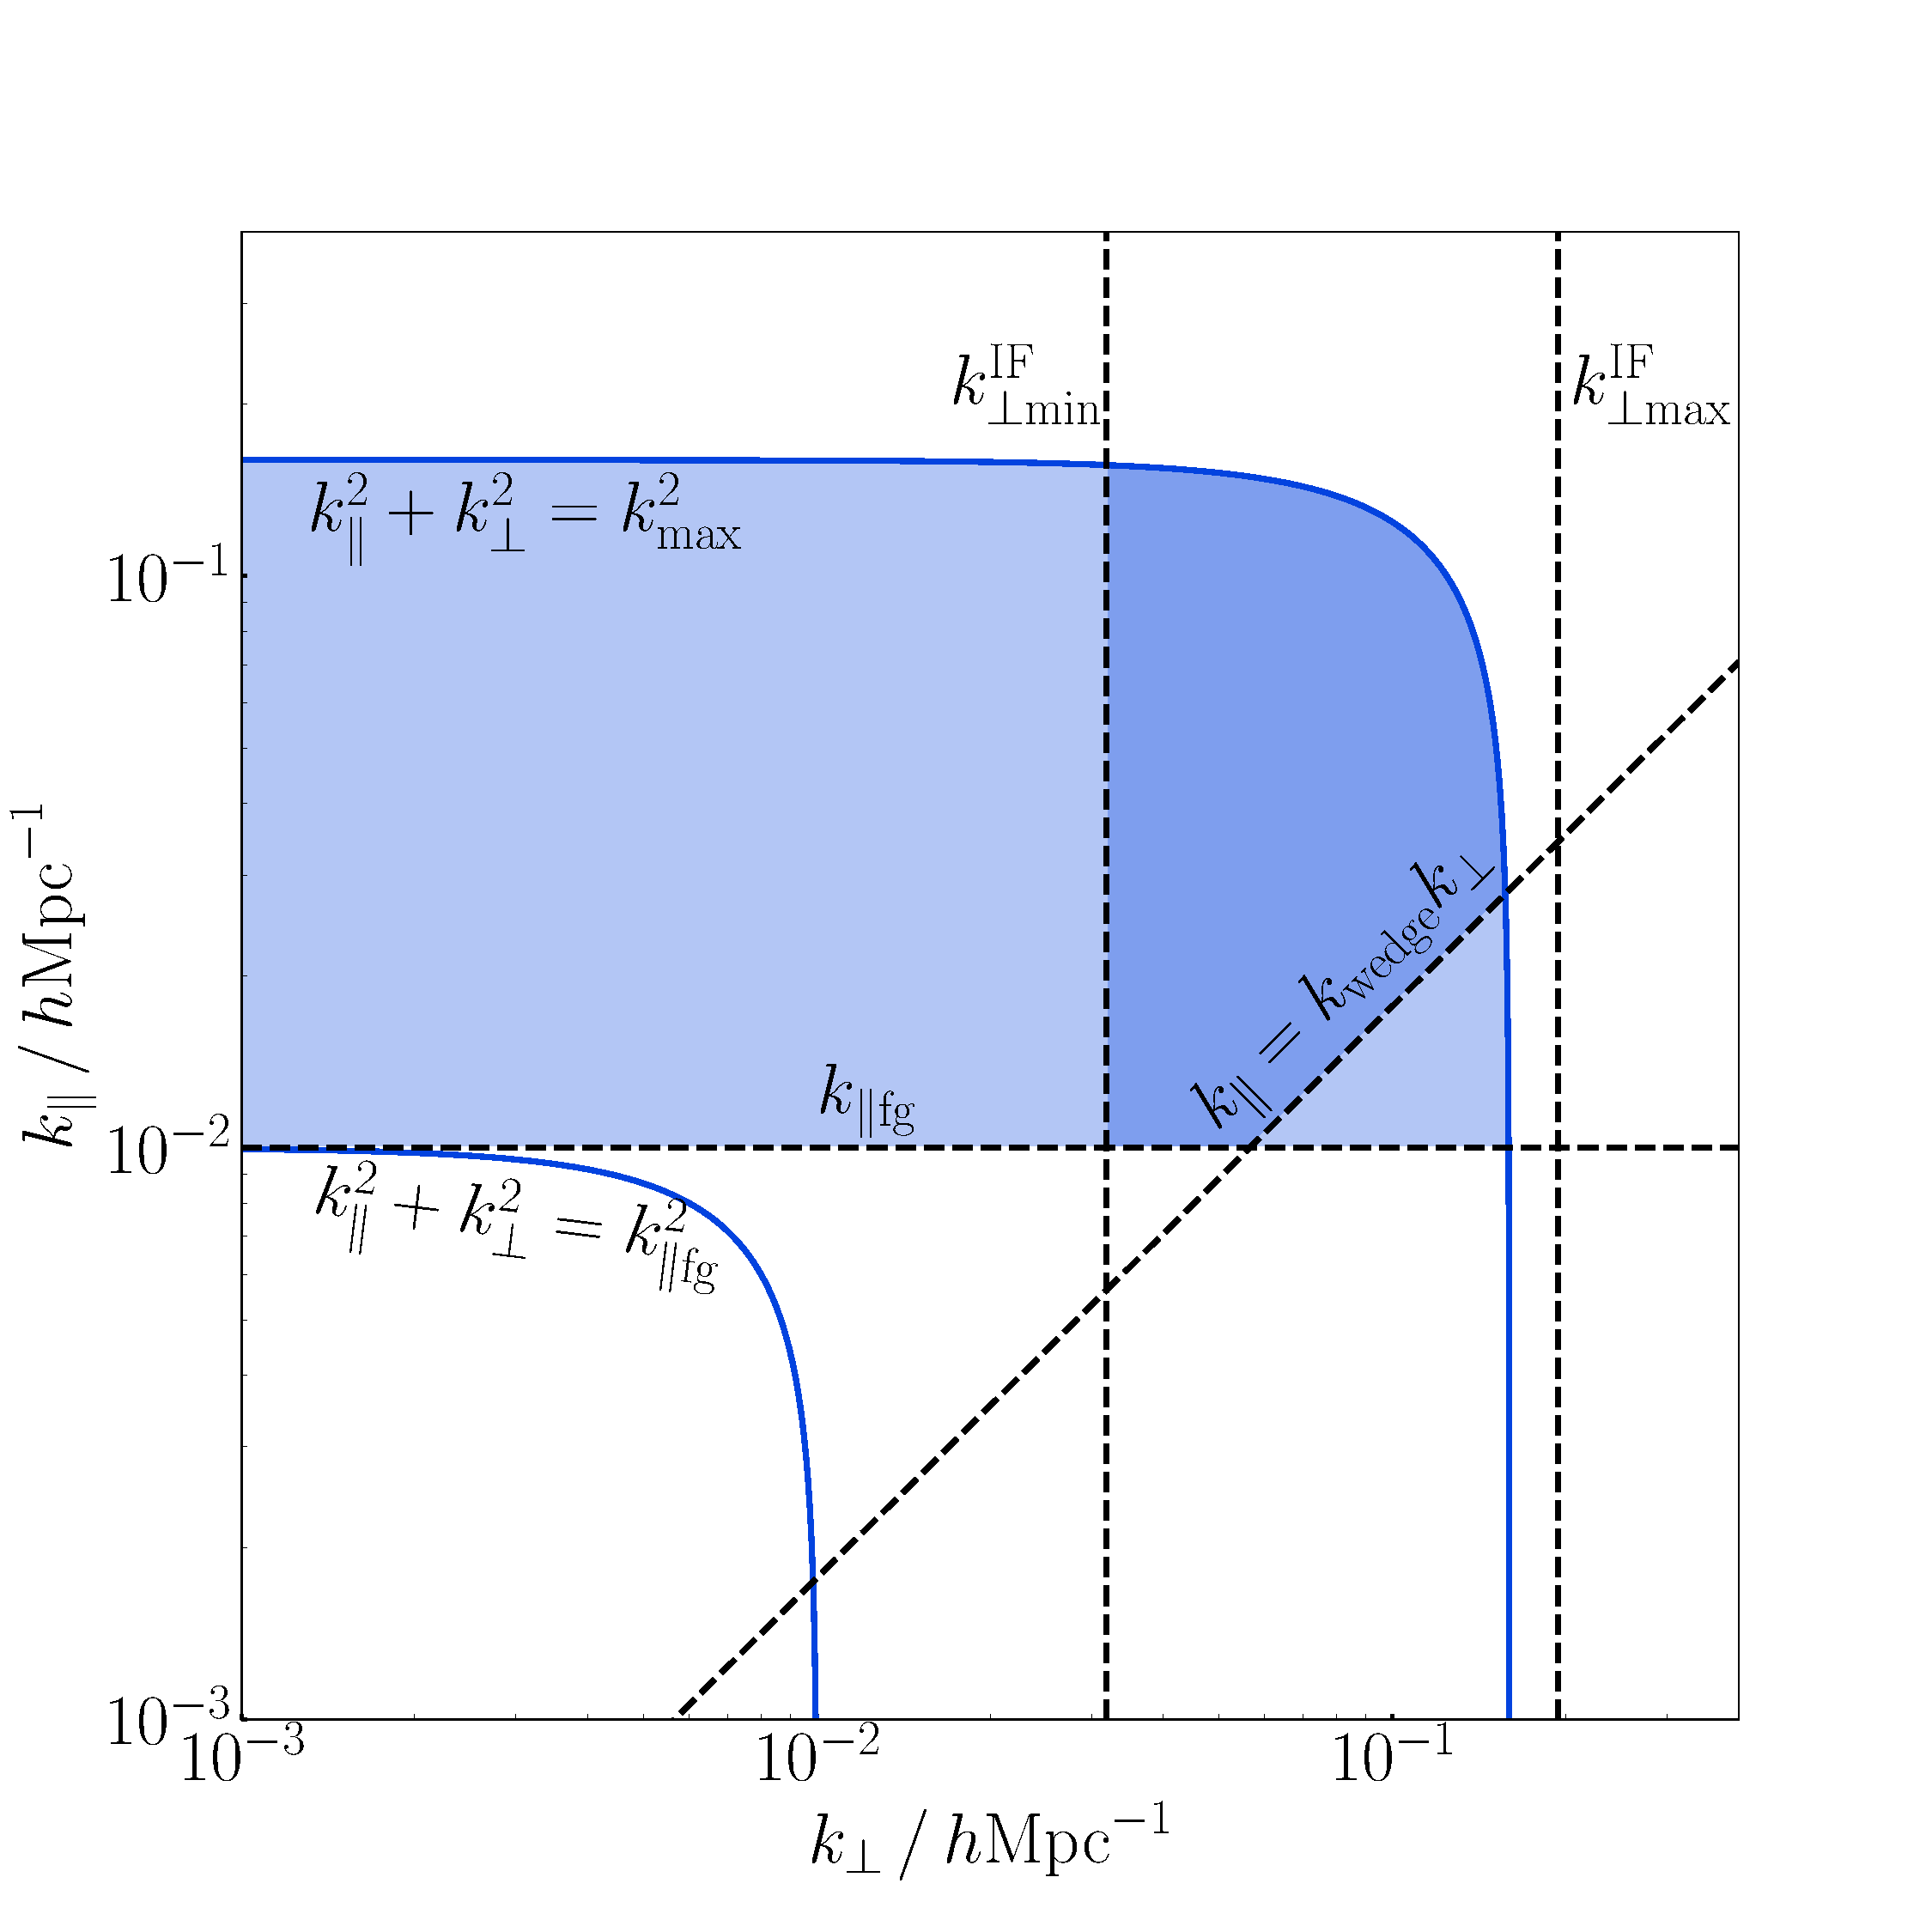
\includegraphics[width=.49\textwidth]{fig/kplane}
%\vspace*{-0.5cm}
\caption{Schematic of important scales in the $k_\|,k_\perp$-plane at fixed $z$. Shading indicates the included region for SD mode (light) and IF mode (dark).}\label{kplane}
\end{figure}

In principle, the maximum wavelength probed by HI intensity surveys at redshift $z$ is $2\pi/k_\mathrm{f}(z)$, where the fundamental mode $k_\mathrm{f}$ is determined by the comoving volume of the redshift bin, via equation~\ref{eq:kfundamental}. 
However, foreground cleaning imposes on both SD- and IF-mode surveys the  limiting minimum radial wavenumber $k_{\|\mathrm{fg}}$, given by~\eqref{kfgpar}. Since $k^2=k_\|^2+k_\perp^2$, this means that  
\begin{equation} \label{eq:kmin}
k>k_{\|\mathrm{fg}} \quad \mbox{which implies}\quad k >  k_\mathrm{min}= \mathrm{max}\,\left\{ k_\mathrm{f}(z), k_{\|\mathrm{fg}} \right\}\,.
\end{equation}
In IF-mode surveys there is a further minimum wavenumber, corresponding to the maximum angular scale that can be probed. This limit depends on the minimum baseline and is given by~\cite{Bull:2014rha,Alonso:2017dgh,Karagiannis:2019jjx,Durrer:2020orn},
\begin{equation} \label{kifmin}
k_{\perp \mathrm{min}}^\mathrm{IF}(z) = \frac{2\pi}{r(z)\,\theta_\mathrm{b}(z)}\,.
\end{equation}
Since $k>k_\perp$, we have
\begin{equation} \label{kminif}
k > k_\mathrm{min} = \mathrm{max}\,\left\{ k_{\perp \mathrm{min}}^\mathrm{IF}(z), k_\mathrm{f}(z), k_{\|\mathrm{fg}} \right\} \quad \mbox{for IF surveys}.
\end{equation}
The scales from foreground cleaning and the maximum and minimum scales are shown schematically in Figure \ref{kplane}. This does not include the effects of the beam in SD mode; 
see Figure~\ref{pnoise}.
%
%
\subsection{Instrumental noise}\label{ssec:inoise}
%
In HI intensity mapping for the scales and redshifts we consider, the shot noise is much smaller than the instrumental noise for next-generation surveys\footnote{{For the futuristic PUMA (Full) survey, the noise is low enough to be comparable to the shot noise \cite{Chen:2018qiu}.}} and can be safely neglected \cite{Castorina:2016bfm,Villaescusa-Navarro:2018vsg}. 
The noise power spectrum for the fractional temperature perturbation is then determined by instrumental noise and is given by~\cite{Bull:2014rha,Alonso:2017dgh}:\footnote{It is also possible to put the beam factor $\beta$ in the signal, rather than in the noise; see e.g. \cite{Bernal:2019jdo} for a discussion.}
\begin{equation}
{P}_{\mathrm{noise}}(z) = \frac{2\pi f_{\mathrm{sky}}}{\nu_{21} t_{\mathrm{tot}}} \, \frac{(1+z) r(z)^{2} }{\cH(z) }\,\left[\frac{T_{\mathrm{sys}}(z)}{\bar{T}_{\hi}(z)}\right]^2\, \frac{\alpha(z,k_\perp)}{\beta(z,k_\perp)^2}
~~~ h^{-3}\mathrm{Mpc}^{3} \,. 
\label{e2.24}
\end{equation}
Here $t_\mathrm{tot}$ is the total observing time, and  the system temperature may be modelled as~\citep{Ansari:2018ury}:
\begin{equation}
T_{\mathrm{sys}}(z) = T_\mathrm{d}(z)+T_\mathrm{sky}(z) =T_\mathrm{d}(z) + 2.7 + 25\left[\frac{400\,\mathrm{MHz}}{\nu_{21}} (1+z)\right]^{2.75} ~ \mathrm{K}, \label{e2.25}
\end{equation} 
where $T_\mathrm{d}$ is the dish receiver temperature. (We consider only dish arrays.)

In~\eqref{e2.24}, the dish density factor $\alpha$ and the effective beam $\beta$ depend on the survey mode as follows~\cite{Bull:2014rha, Obuljen:2017jiy, Ansari:2018ury, Jalilvand:2019bhk, Durrer:2020orn},
\begin{align}
\alpha_\mathrm{SD} &= \frac{1}{N_\mathrm{d}}\,,\qquad\qquad\qquad\qquad  \beta_\mathrm{SD}= \exp\left[-\frac{k_\perp^2 r(z)^2\theta_\mathrm{b}(z)^2}{16\ln 2} \right], \label{sdn} \\
\alpha_\mathrm{IF} &=\left[ \frac{\lambda(z)^2}{A_\mathrm{e}}\right]^2 \frac{1}{n_\mathrm{b}(z,k_\perp)}
\,,\quad~  \beta_\mathrm{IF}= \theta_\mathrm{b}(z)\,. \label{ifn}
\end{align}
Here $N_\mathrm{d}$ is the number of dishes  and $A_\mathrm{e}$ is the effective beam area,
\begin{equation} \label{aeff}
A_\mathrm{e} = 0.7 A_\mathrm{d}\,, \quad A_\mathrm{d} = \frac{\pi}{4} D_\mathrm{d}^2\,.
\end{equation}
The dimensionless $n_\mathrm{b}$ is the baseline density in the image plane (assuming azimuthal symmetry), which is determined by the array distribution. The total number of baselines is $\int \ud^2{\bm u}\,n_\mathrm{b}(u) = N_\mathrm{d}(N_\mathrm{d}-1)/2.$
A physical baseline length $L$ is related to an image-plane scale $u$ as
\begin{equation}
L = u\lambda = \frac{k_\perp r}{2\pi}\,\lambda\,.
\end{equation}
Then the image-plane and physical distributions of the array are related by~\cite{Ansari:2018ury},
\begin{equation} \label{nbphy}
n_\mathrm{b}(z,u) = \lambda(z)^2\, n_\mathrm{b}^\mathrm{phys}(L)\,.
\end{equation}
%
%
\subsection{Future 21cm IM surveys}
%
We consider surveys proposed for the following dish arrays:
\begin{itemize}
\item 
SD mode:  MeerKAT, 
SKA1-MID.
\item
IF\ mode: HIRAX,
PUMA (Petite). 
\end{itemize}
The survey specifications are given in Table~\ref{tab:hisurveyspecs}, based on~\cite{Santos:2017qgq, Bacon:2018dui, Slosar:2019jwd,Karagiannis:2019jjx,Castorina:2020zhz}. Limiting wavenumbers for large wavelengths are shown for these surveys in Figure~\ref{figmin}: the fundamental wavenumber~\ref{eq:kfundamental}, the minimum radial wavenumber~\eqref{kfgpar} from foreground cleaning and the IF-mode minimum wavenumber~\eqref{kifmin}.


\begin{table}[ht]
\footnotesize
\centering
\caption{\label{tab:hisurveyspecs} HI intensity mapping survey specifications. 
(For *, see Table~\ref{tab:skasystemp}.)} 
\vspace*{0.2cm}
\begin{tabular}{|lccccccc|} \hline
Survey & Redshift range & $f_\mathrm{sky}$ & $t_{\mathrm{tot}}$  & $T_{\mathrm{d}}$ & $D_\mathrm{d}$ & $N_\mathrm{d}$ & $D_\mathrm{max}$ \\
&  & & [$10^{3}$ hr] & [K]  & [m] & & {[m]} \\
\hline\hline 
MeerKAT L Band   & 0.10--0.58 & 0.10 & 4  & * & 13.5 & 64 & -- \\
MeerKAT UHF Band & 0.40--1.45 & 0.10 & 4  & * & 13.5 & 64  & --  \\
SKA1-MID Band 1  & 0.35--3.05 & 0.48 & 10 & * & 15.0 & 197  & --  \\
SKA1-MID Band 2  & 0.10--0.49 & 0.48 & 10 & * & 15.0 & 197  & --  \\
HIRAX            & 0.75--2.00 & 0.36 & 10 & 50 & 6.0  & 1024  & 270\\
PUMA (Petite)    & 2.00--6.00 & 0.50 & 40 & 50 & 6.0  & 5000 & 600 \\
\hline
\end{tabular}
\end{table}

\vspace*{-0.5cm}
\begin{table}[ht]
\centering
\caption{\label{tab2} Parameters in~\eqref{e3.4} (from \cite{Ansari:2018ury}).} 
\vspace*{0.2cm}
\begin{tabular}{|lcccccl|} \hline
Survey & $a$ & $b$ & $c$  & $d$ & $e$ & $N_\mathrm{s}$  \\ \hline\hline 
HIRAX & 0.4847 & $-0.3300$ & 1.3157 & 1.5974 & 6.8390 & 32  \\
PUMA (Petite) & 0.5698 & $-0.5274$ & 0.8358 & 1.6635 & 7.3177 & {100} \\
\hline
\end{tabular}
\end{table}

For the system temperature, we use the results of measurements and simulations for MeerKAT and SKA1-MID, given below in Table~\ref{tab:skasystemp} and Figure~\ref{fig:Tsysforska}. For HIRAX and PUMA, we use the fit~\eqref{e2.25}. 

\vspace*{-0.5cm}
\begin{table}[! ht]
\centering
\caption{\label{tab:skasystemp} System temperatures for MeerKAT and SKA1-MID, used in Figure~\ref{fig2} (from \cite{Fonseca:2019qek}).} 
\vspace*{0.2cm}
  \begin{tabular}{|l|l|l|l|l|l|l|l|}
    \hline
      \multicolumn{2}{|c|}{MeerKAT L Band} &
      \multicolumn{2}{c|}{MeerKAT UHF Band} &
      \multicolumn{2}{c|}{SKA1-MID Band 1} & 
      \multicolumn{2}{c|}{SKA1-MID Band 2} \\
      \hline \hline
    $~~~~z~~$ & $~~T_\mathrm{sys}\;/\;\mathrm{K}~~~$ & $~~~z~$ & $~~~~T_\mathrm{sys}\;/\;\mathrm{K}~~$ & $~~~z~$ & $~~T_\mathrm{sys}\;/\;\mathrm{K}~~$ & $~~~~z~~$ & $~~T_\mathrm{sys}\;/\;\mathrm{K}~~$ \\
    \hline
    
  %& & & & & & & \\
  
     0.136 & ~~~~19.2 & 0.420 & ~~~~~~20.3 & 0.403 & ~~~~27.2 & 0.115 & ~~~~16.4 \\
    
     0.183 & ~~~~19.7 & 0.495 & ~~~~~~21.0 & 0.470 & ~~~~26.9 & 0.168 & ~~~~16.6 \\
    
     0.235 & ~~~~20.3 & 0.578 & ~~~~~~21.7 & 0.539 & ~~~~26.8 & 0.223 & ~~~~16.8 \\
    
     0.291 & ~~~~20.9 & 0.671 & ~~~~~~22.5 & 0.612 & ~~~~26.9 & 0.280 & ~~~~17.0 \\
    
     0.352 & ~~~~21.5 & 0.775 & ~~~~~~23.5 & 0.767 & ~~~~27.5 & 0.341 & ~~~~17.2 \\
    
    0.420 & ~~~~22.3 & 0.893 & ~~~~~~24.7  & 0.850 & ~~~~28.1 & 0.403 & ~~~~17.6 \\
    
    0.495 & ~~~~23.1 & 1.03 & ~~~~~~26.1   & 0.938 & ~~~~28.8 & 0.470  & ~~~~18.0 \\
    
    0.578 & ~~~~24.0 & 1.18 & ~~~~~~27.9   & 1.03  & ~~~~29.8 &        &  \\
    
          &          & 1.37 & ~~~~~~30.3   & 1.12  & ~~~~30.8 &        &  \\
     
          &          & 1.45 & ~~~~~~31.5   & 1.22  & ~~~~32.1 &        &  \\
    
          &          &      &              & 1.33  & ~~~~33.5 &        &   \\
    
          &          &      &              & 1.44  & ~~~~35.2 &        &    \\
    
          &          &      &              & 1.55  & ~~~~37.1 &        &   \\
    
          &          &      &              & 1.67  & ~~~~39.2 &        &   \\
    
          &          &      &              & 1.80  & ~~~~41.6 &        & \\
    
          &          &      &              & 1.93  & ~~~~44.2 &        &  \\
    
          &          &      &              & 2.07  & ~~~~47.2 &        &  \\
    
          &          &      &              & 2.22  & ~~~~50.6 &        &  \\
    
          &          &      &              & 2.37  & ~~~~54.4 &        &  \\
    
          &          &      &              & 2.54  & ~~~~58.6 &        &  \\
    
          &          &      &              & 2.69  & ~~~~63.4 &        &  \\
    
          &          &      &              & 2.87  & ~~~~68.8 &        &  \\
    
          &          &      &              & 3.05  & ~~~~74.8 &        &  \\
    
 %         &          &      &              &       &          &        &  \\
    \hline
  \end{tabular}
\end{table}
% \vspace*{-0.5cm}
 \begin{figure}[!ht]
\centering
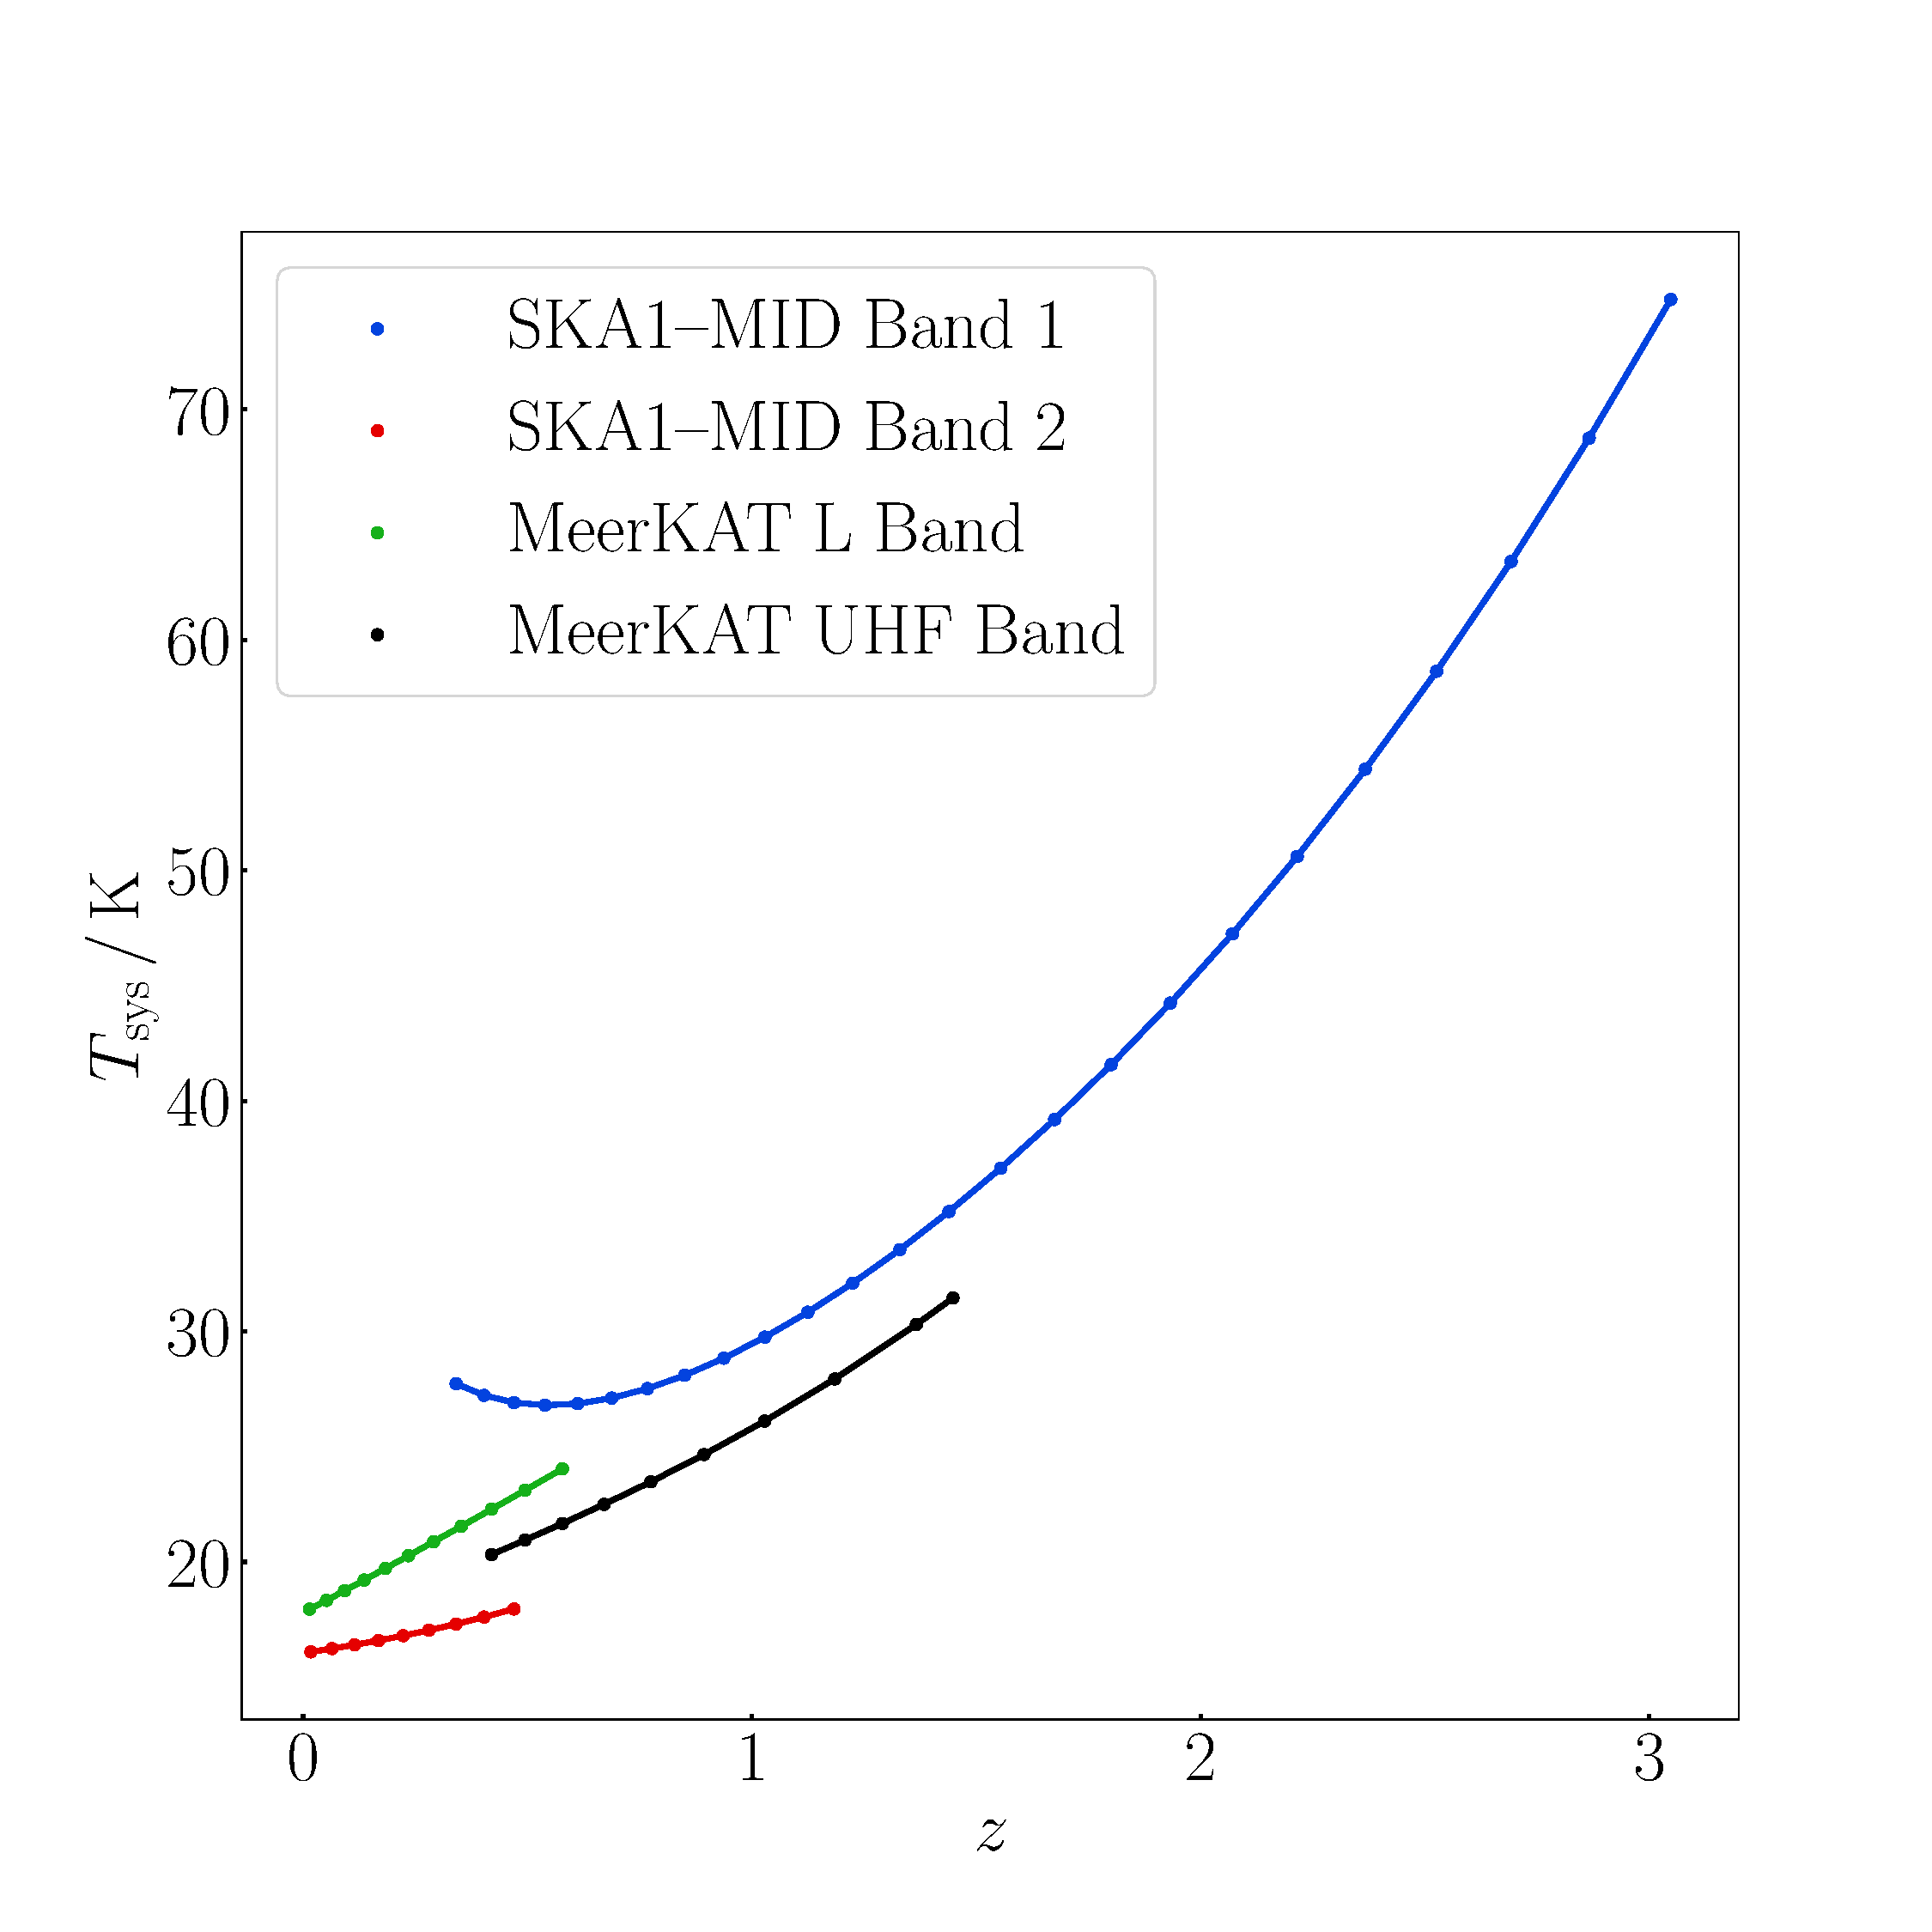
\includegraphics[width=.49\textwidth]{fig/tSys}
% \vspace*{-0.5cm}
\caption{$T_\mathrm{sys}$ for the different frequency bands of MeerKAT and SKA1 (from Table~\ref{tab:skasystemp}).} \label{fig:Tsysforska}
\end{figure}  

In IF mode, HIRAX is assumed to be a square-packed array, while PUMA is taken as hexagonal-packed in a circular area, {with 50\% fill factor}. We follow~\cite{Karagiannis:2019jjx} and use the fitting formula from~\cite{Ansari:2018ury} for the baseline density of such arrays,
\begin{equation}
n_\mathrm{b}^\mathrm{phys}(L) = \left(\frac{N_\mathrm{s}}{D_\mathrm{d}}\right)^2\,\frac{a+b\left(L/L_\mathrm{s}\right)}{1+c\left(L/L_\mathrm{s}\right)^{d}}\,\exp{\left[-(L/L_\mathrm{s})^{e}\right]}\,, \label{e3.4}
\end{equation}
where $L_\mathrm{s} = N_\mathrm{s} D_\mathrm{d}$ and $N_\mathrm{s}^2 = N_\mathrm{d}$.
The parameters in~\eqref{e3.4} are given in Table~\ref{tab2}, and $n_\mathrm{b}^\mathrm{phys}(L)$ is shown in Figure~\ref{nbphys}.
\begin{figure}
\centering
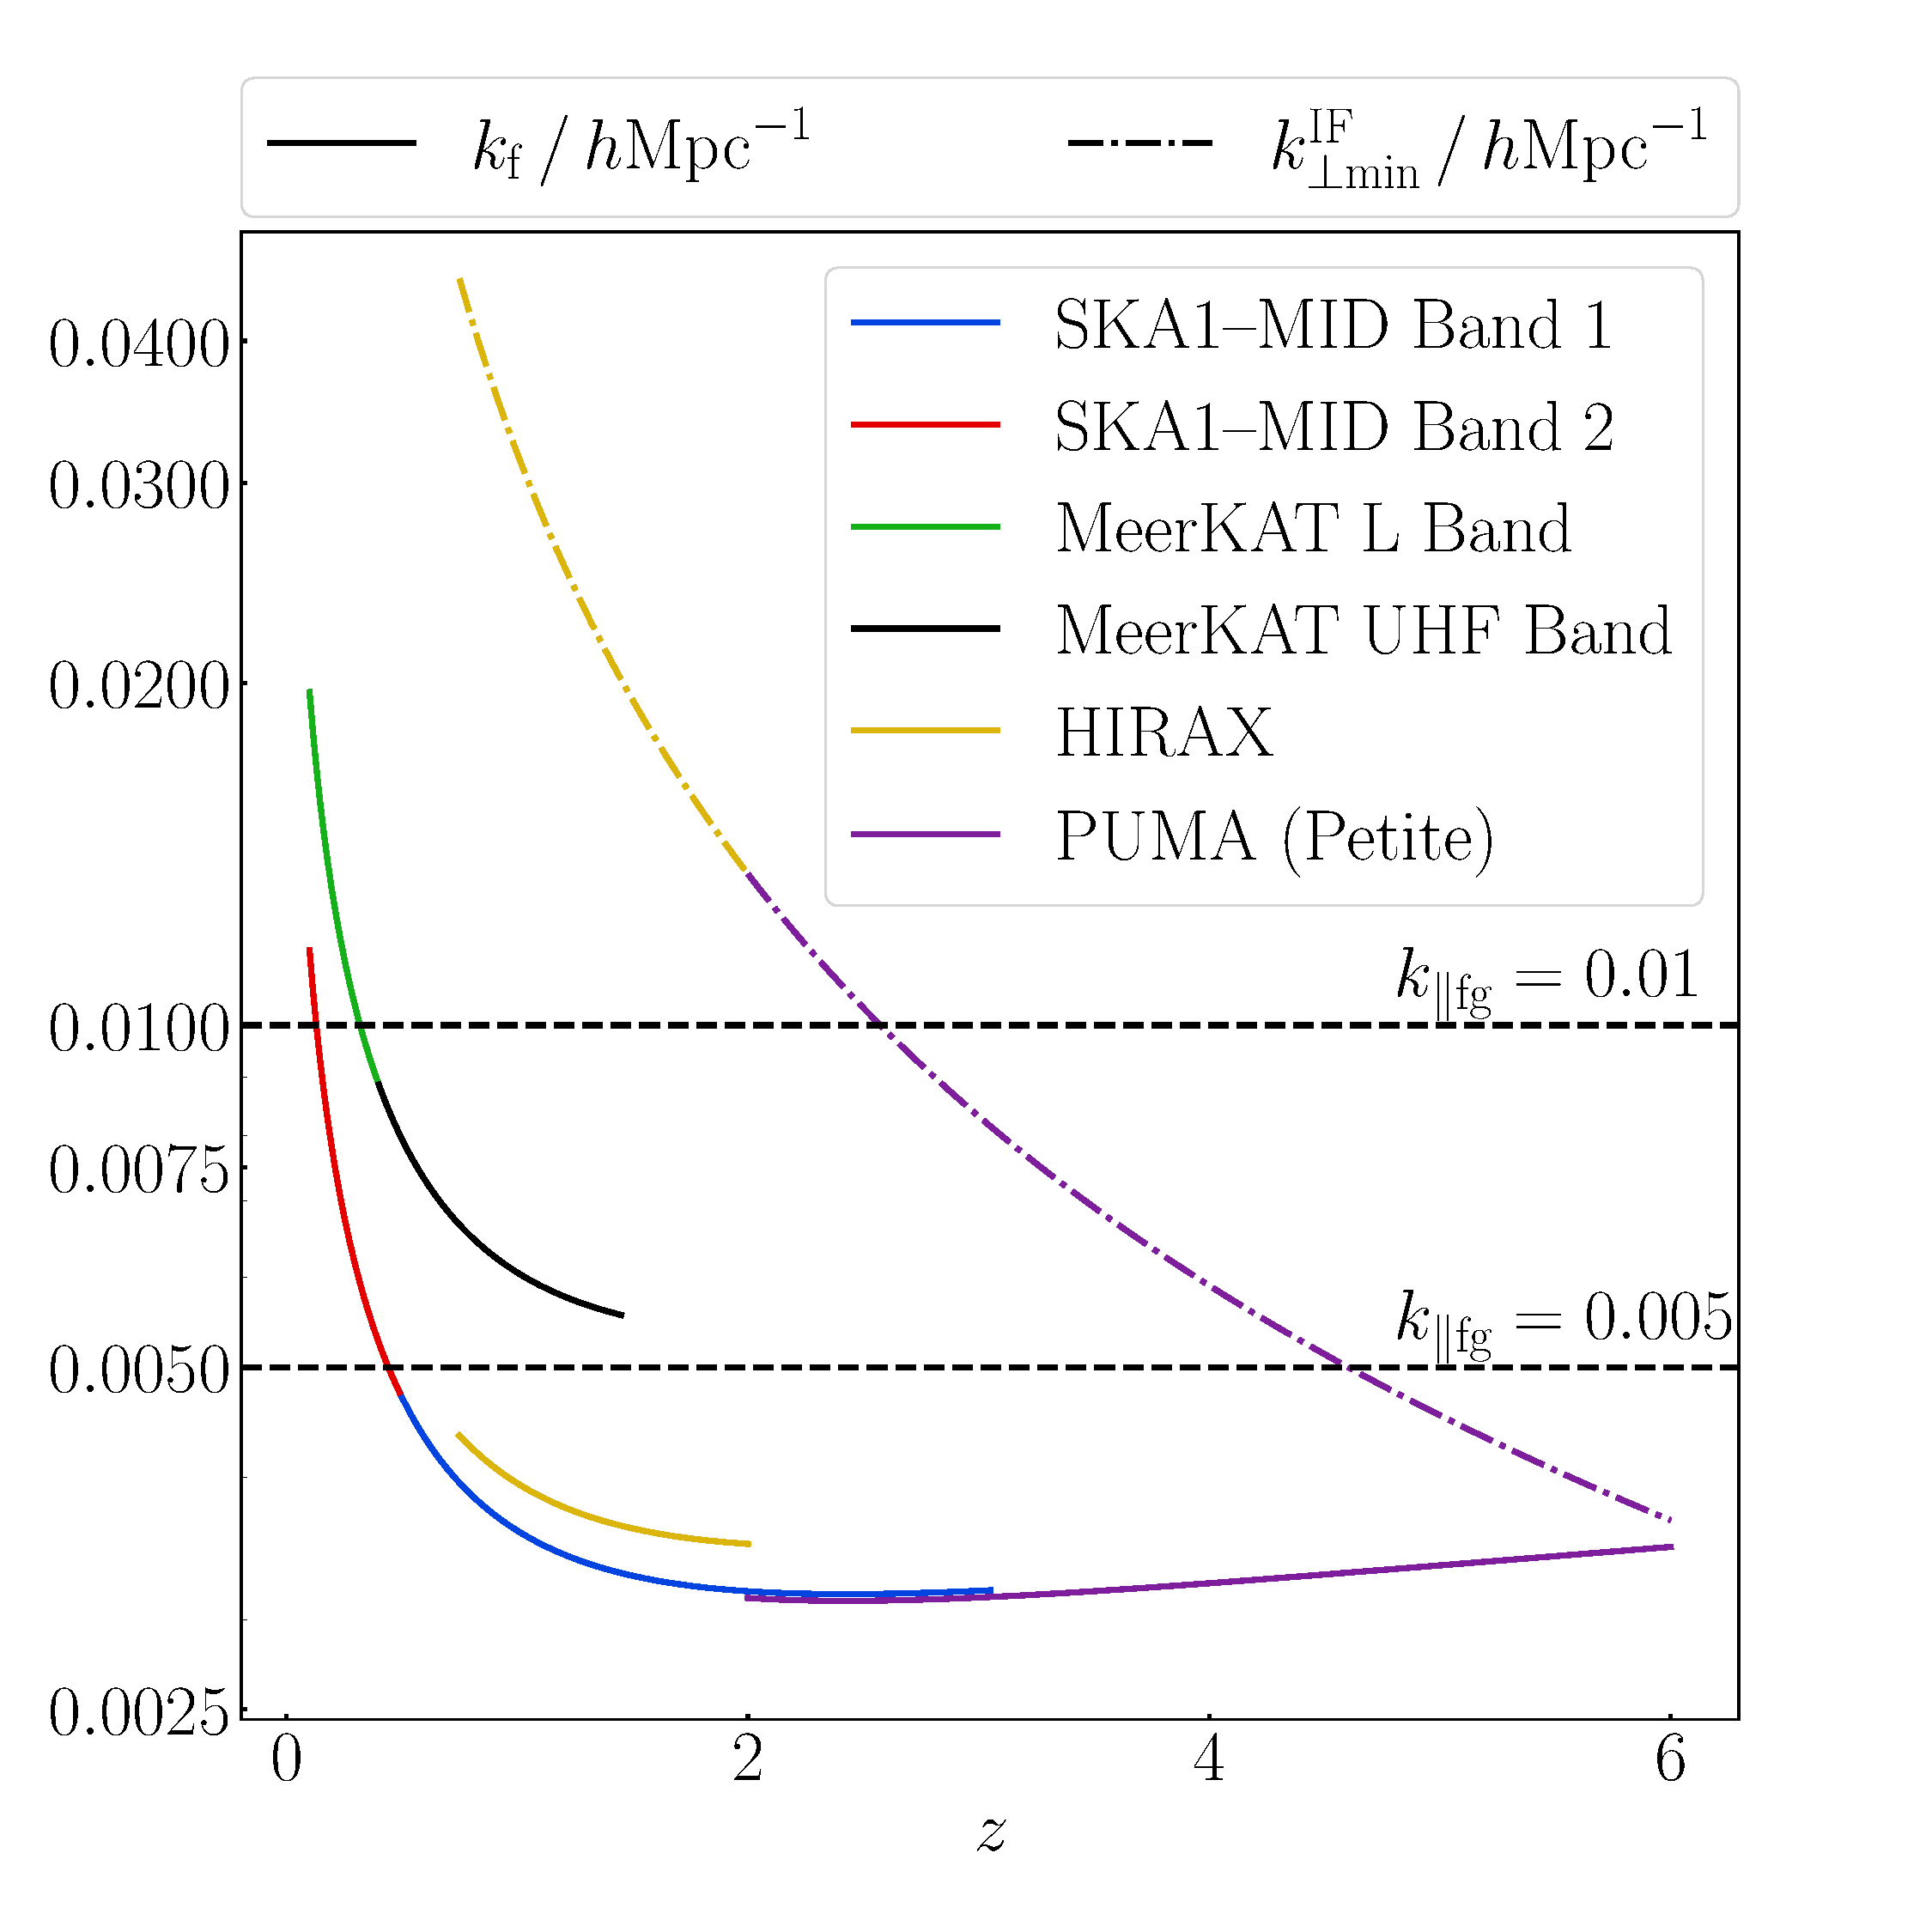
\includegraphics[width=.49\textwidth]{fig/k}
\caption{Minimum wavenumbers for the surveys, where $k$ is subject to~\eqref{kmin} (SD) or~\eqref{kminif} (IF).}\label{figmin}
\end{figure}
\begin{figure}[ht]
\centering
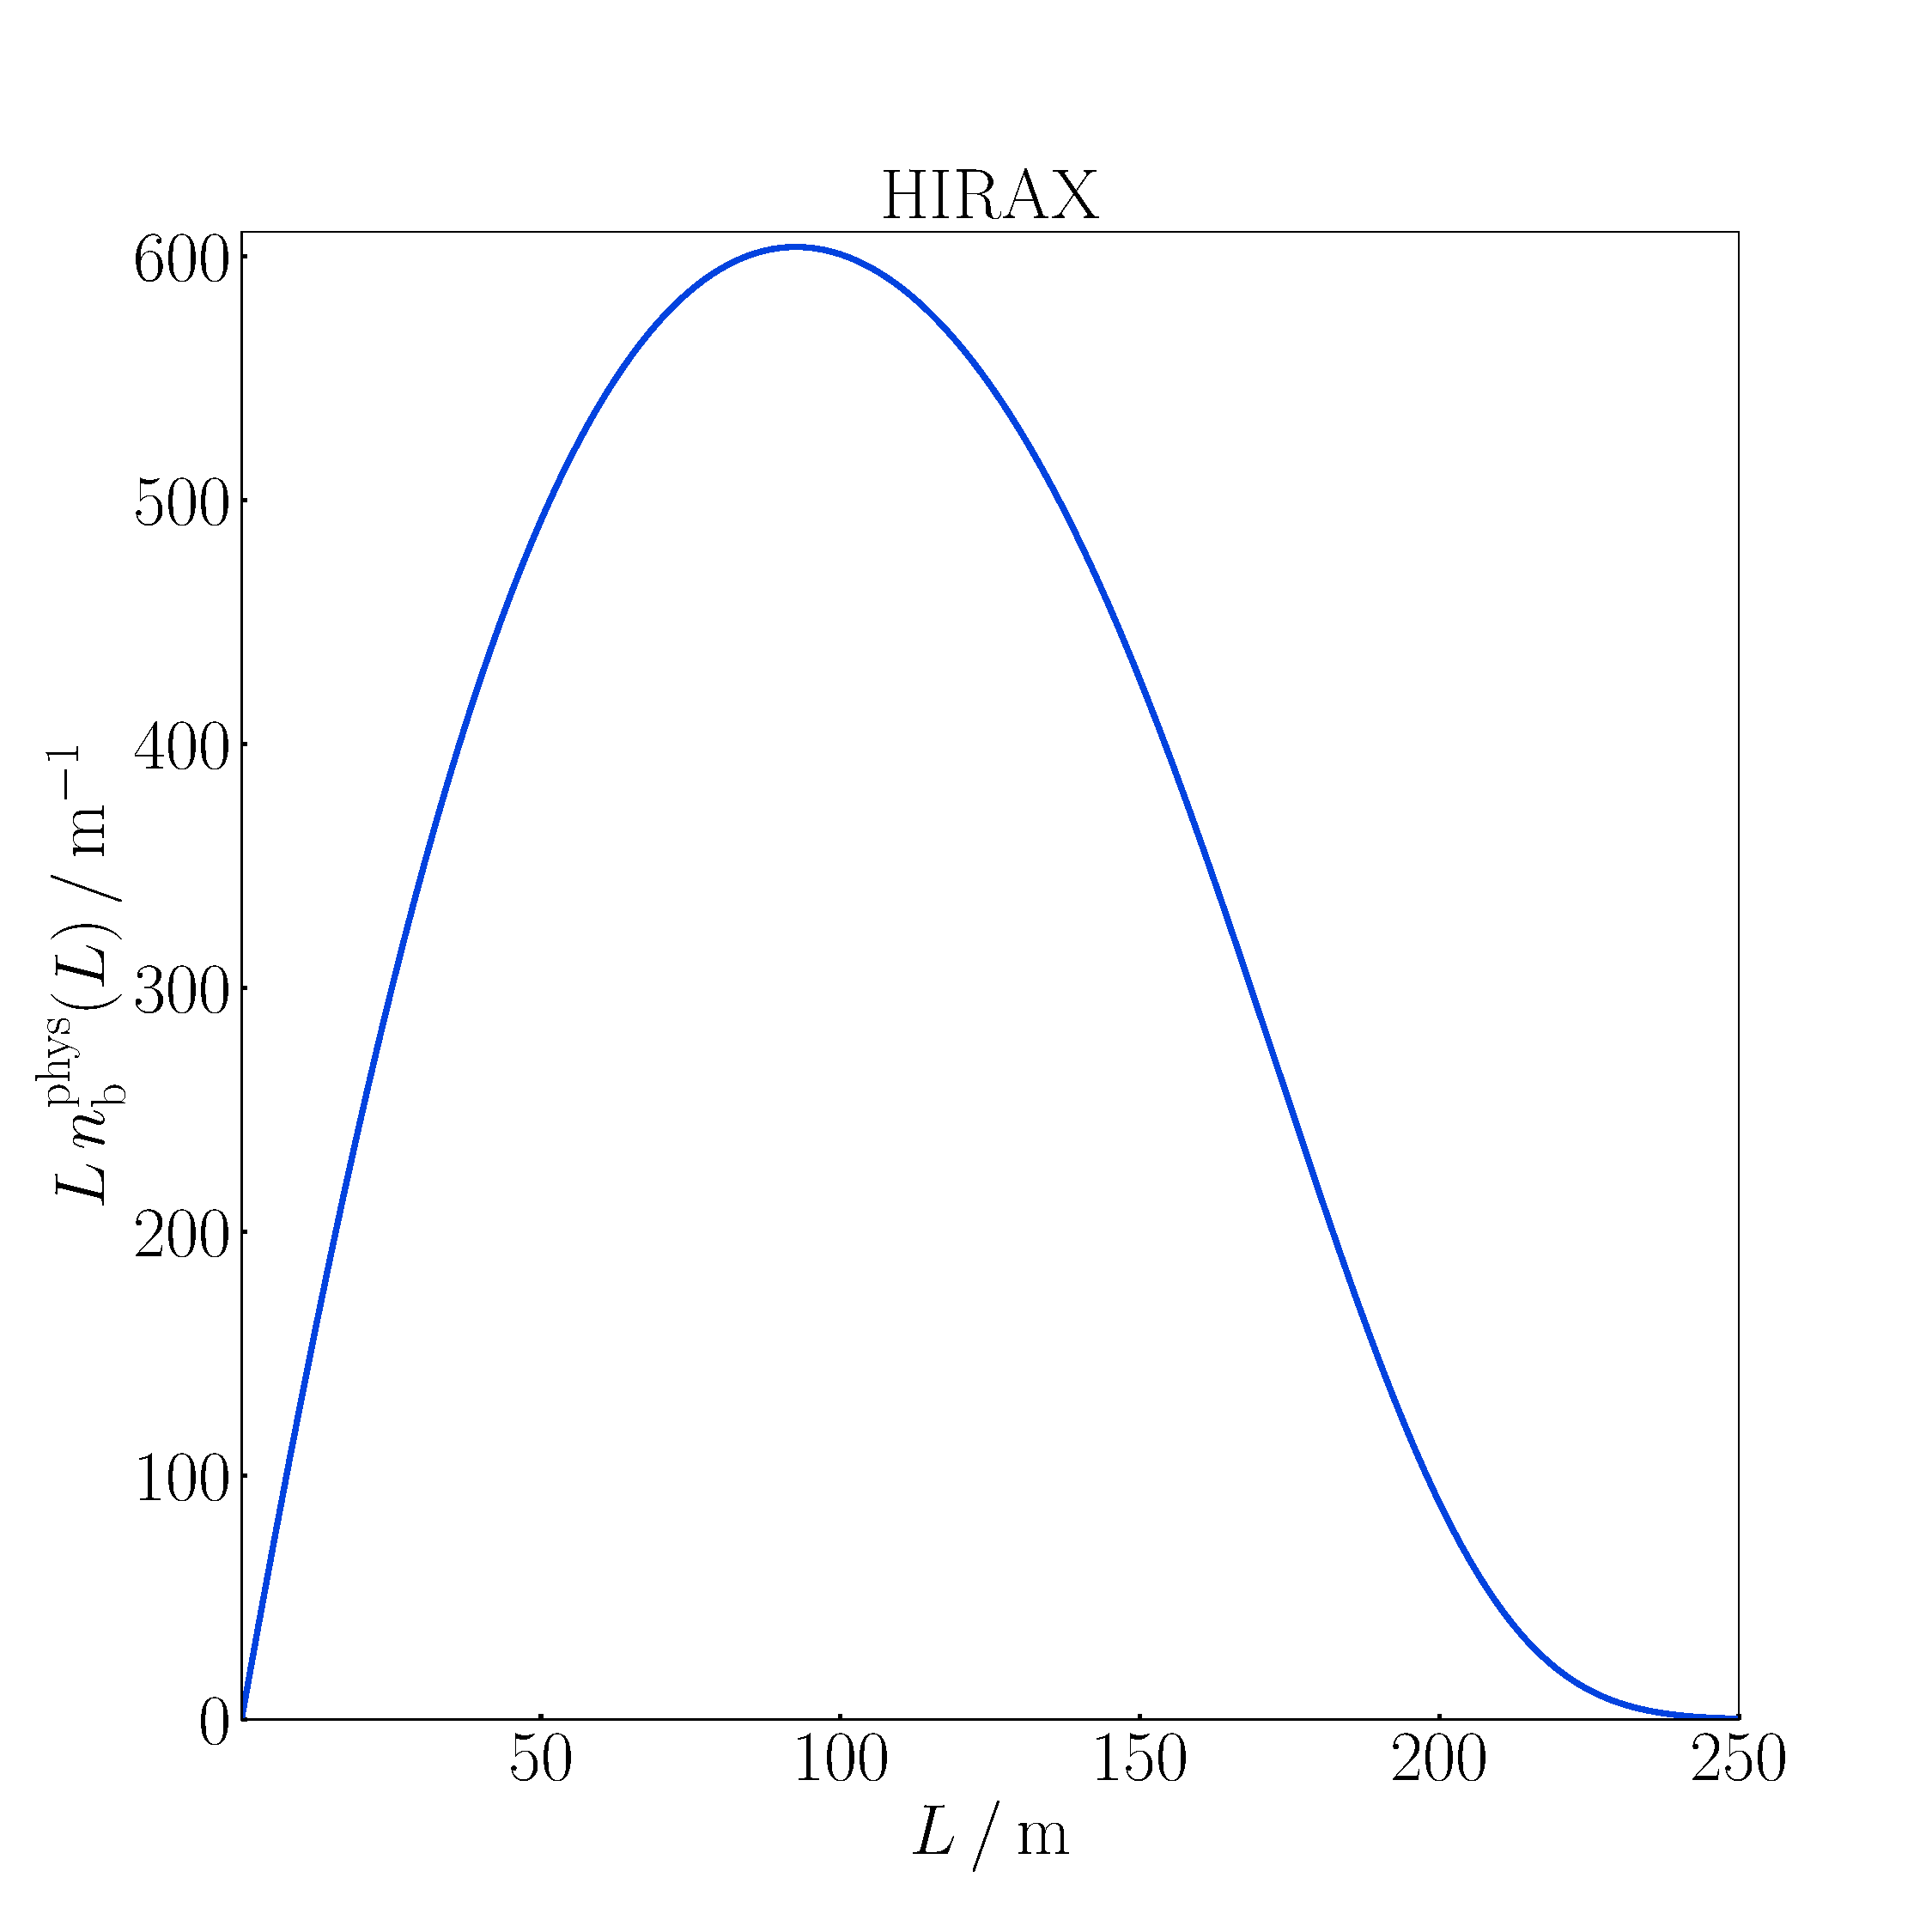
\includegraphics[width=.49\textwidth]{fig/nbHIRAX}
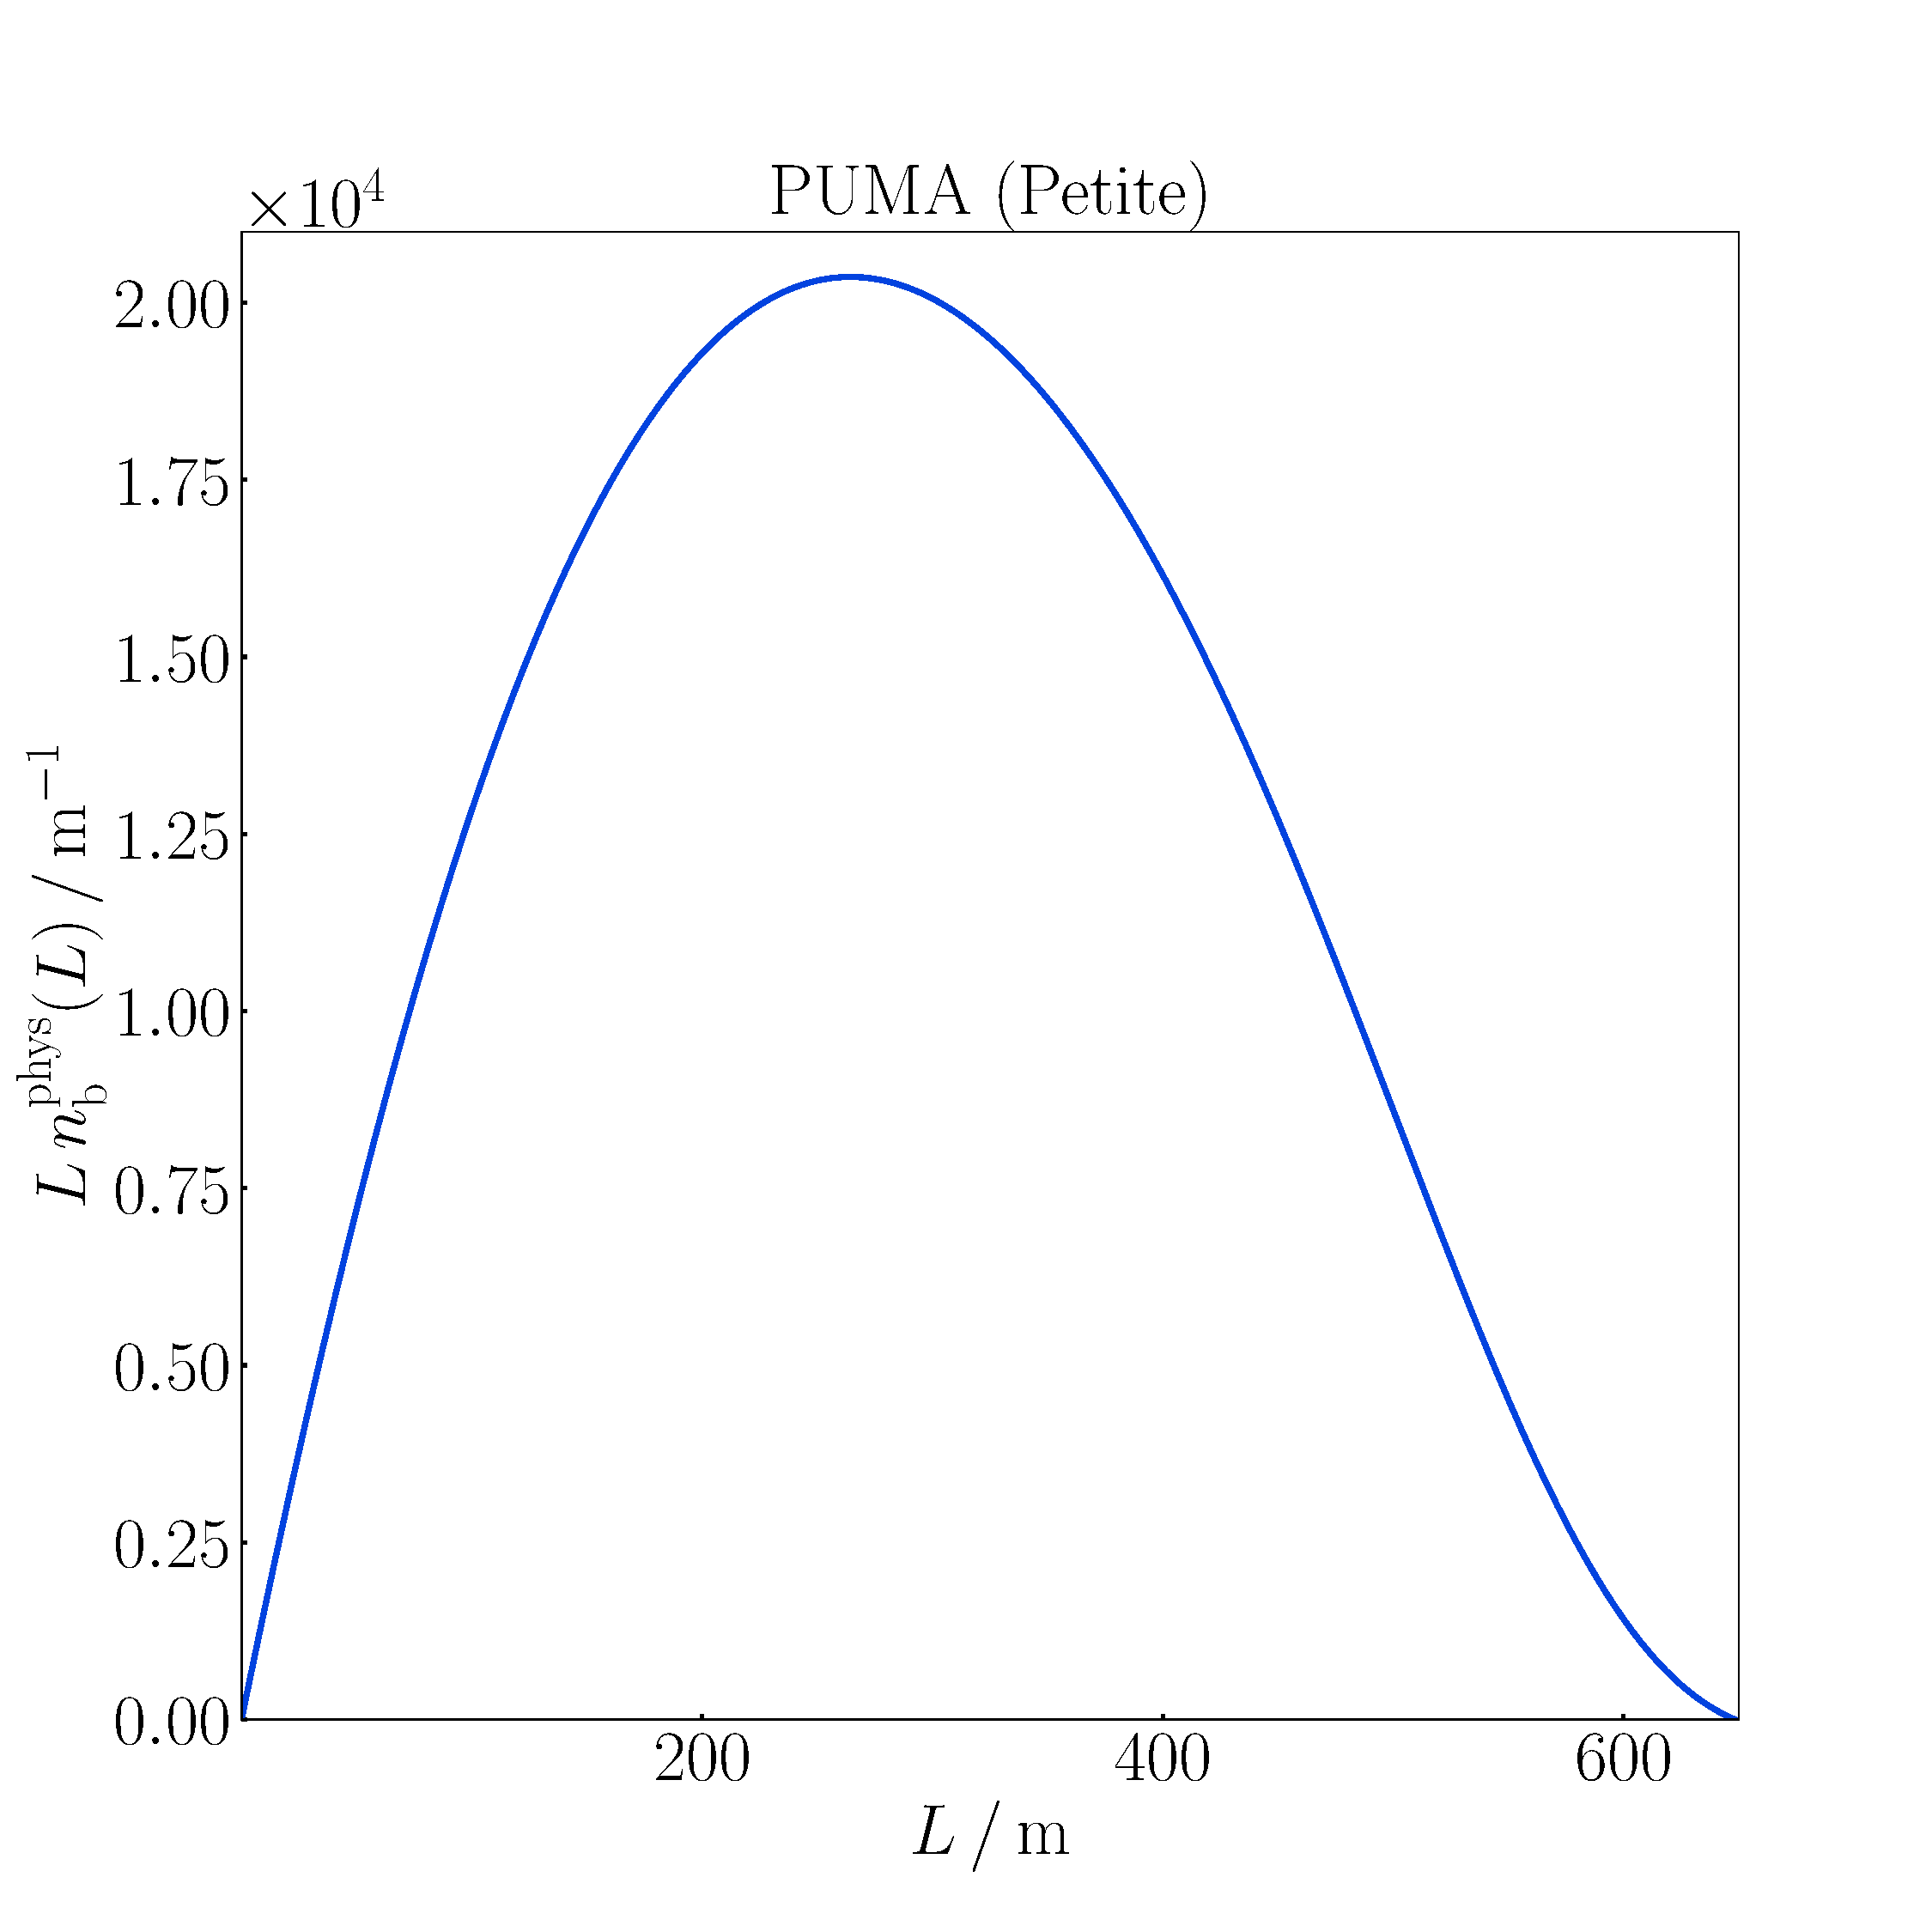
\includegraphics[width=.49\textwidth]{fig/nbPUMAPetite}
\vspace*{-0.5cm}
\caption{Physical baseline density models for HIRAX (left) and PUMA (right).}\label{nbphys}
\end{figure}
\begin{figure}[!ht]
\centering
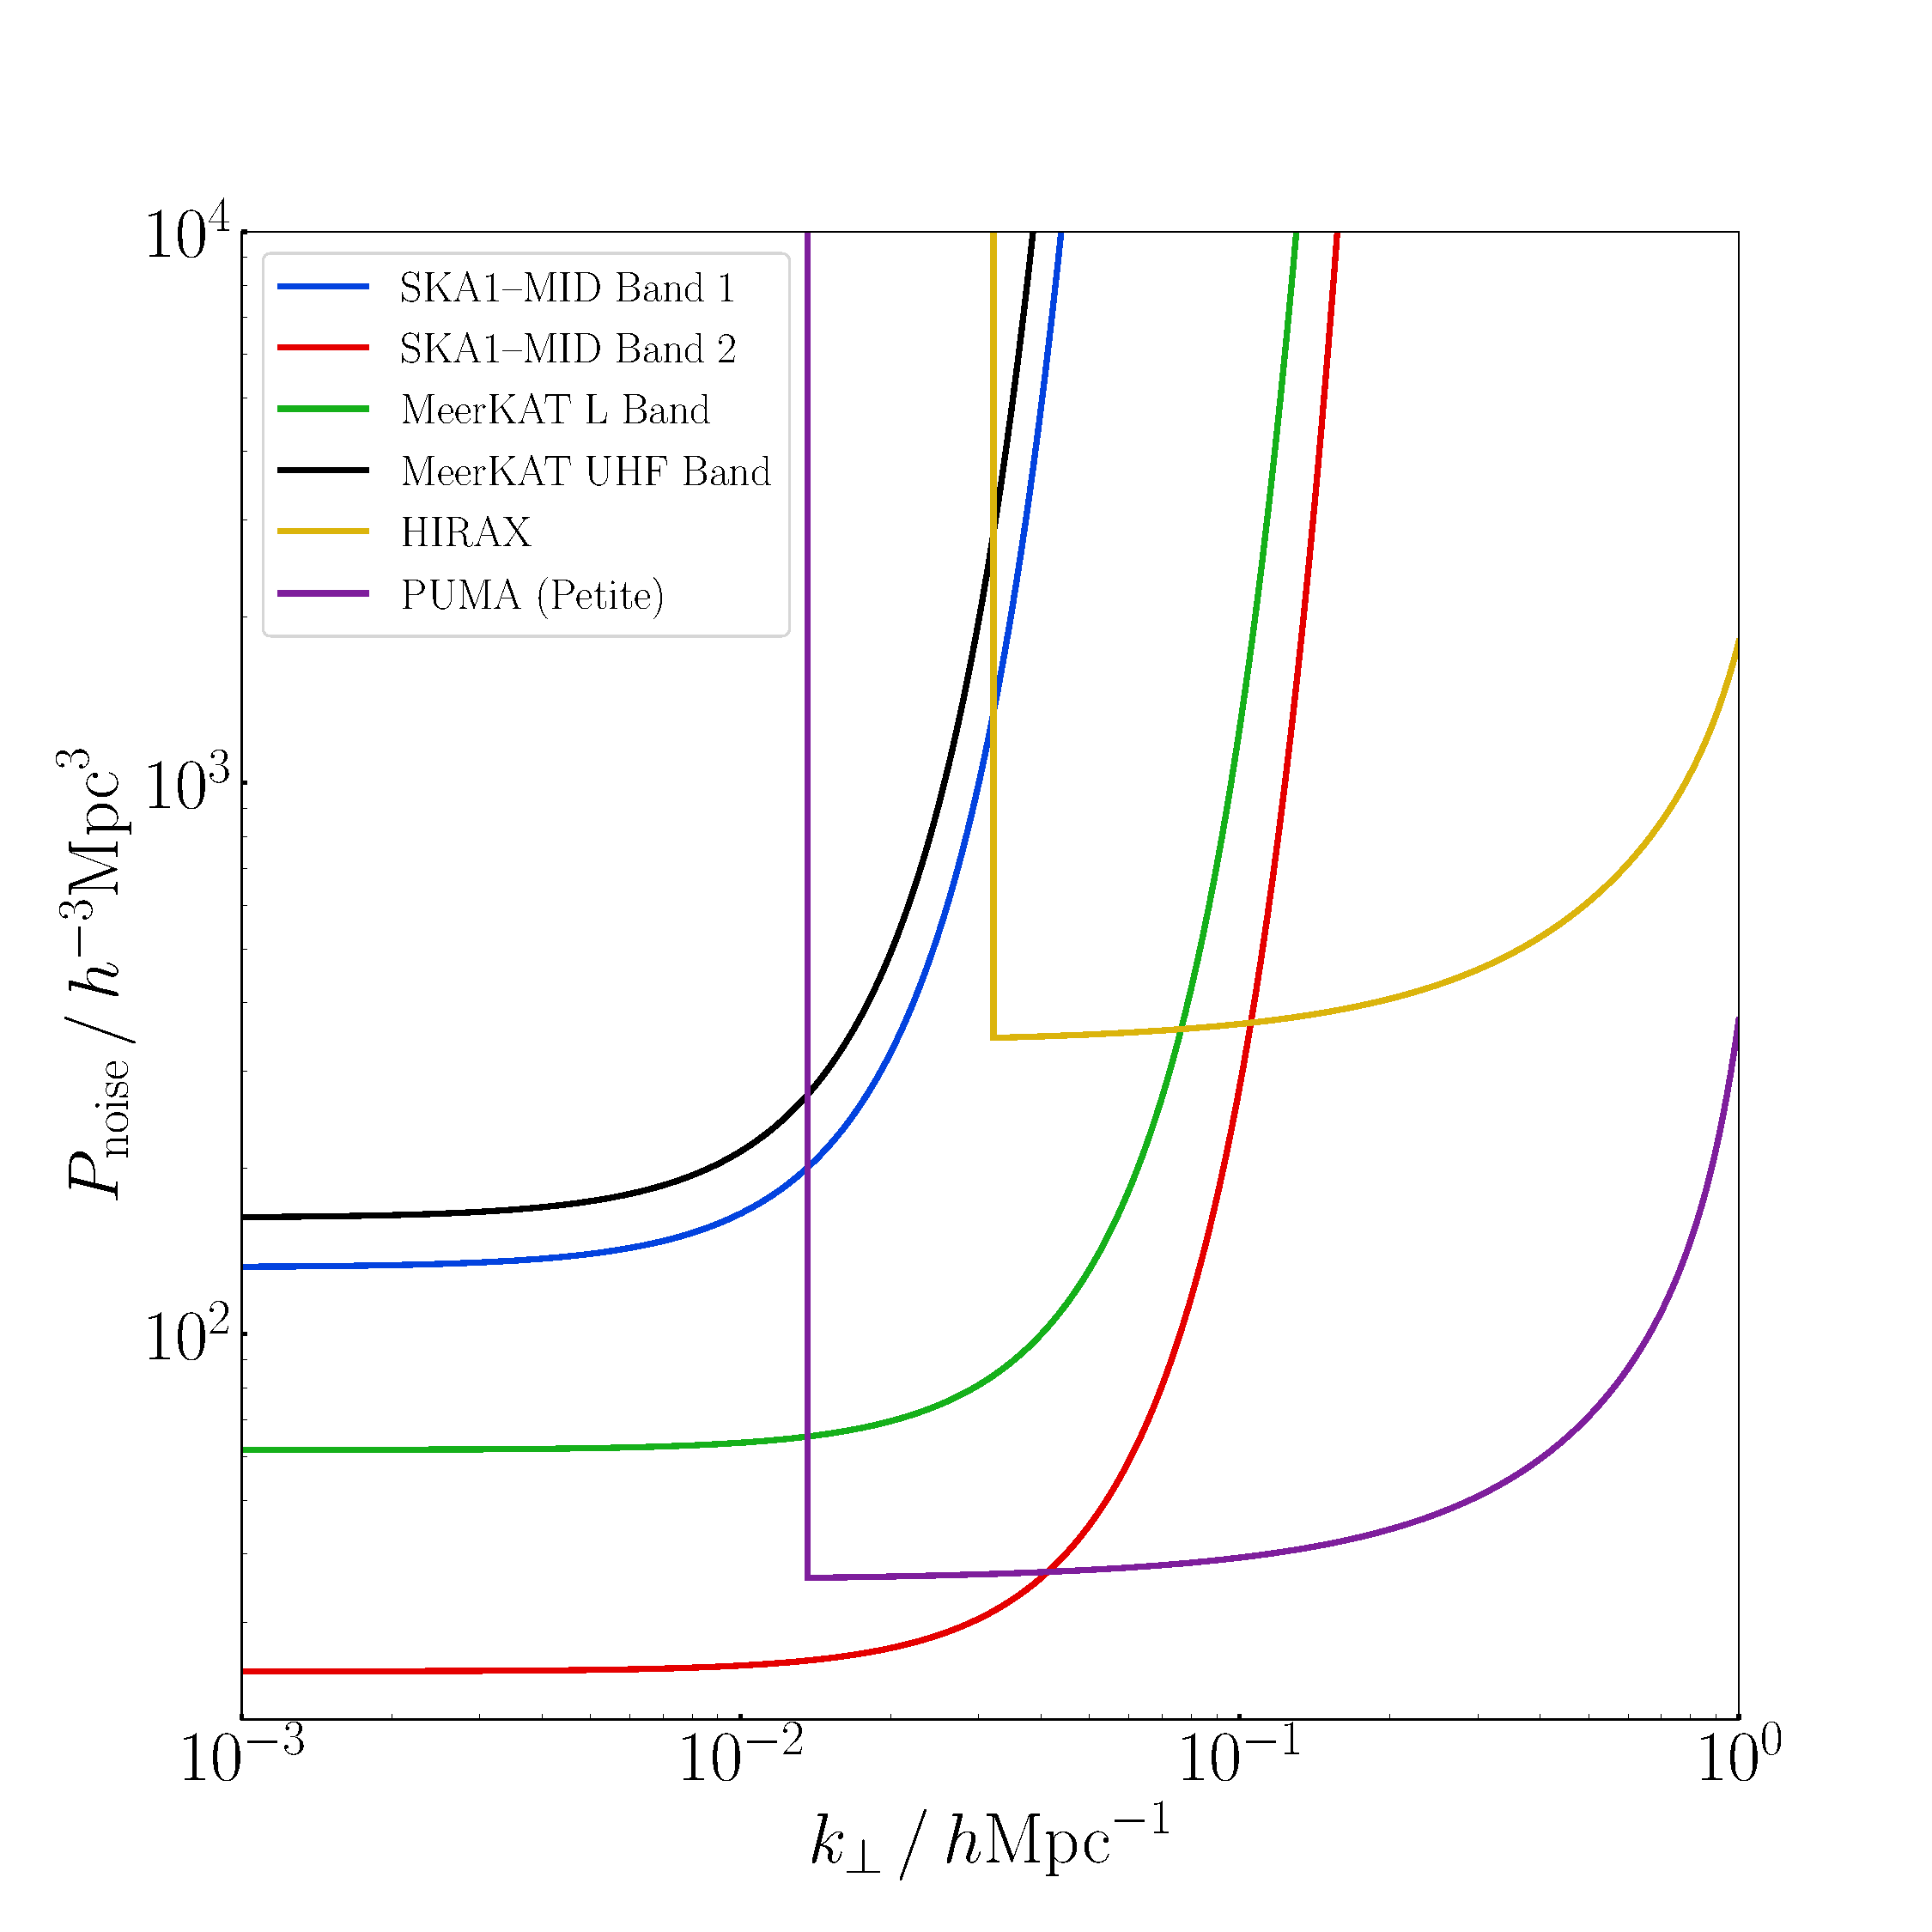
\includegraphics[width=.49\textwidth]{fig/Pnoise}
\vspace*{-0.5cm}
\caption{Noise power spectra of the SD-mode surveys (at $z=0.4$ for low-$z_\mathrm{max}$ bands and $z=1$ for high-$z_\mathrm{max}$ bands) and IF-mode surveys (HIRAX at $z=1$, PUMA at $z=2$).}\label{pnoise}
\end{figure}

In the case of PUMA, we take account of the 50\% fill factor as follows. We use double the number of dishes to define $N_\mathrm{s}$ for the computation of~\eqref{e3.4}, i.e. $N_\mathrm{s}^2= 2\times 5000$. Then  we  remove half of the dishes without changing the baseline, i.e. without changing the shape and ground-area of the array.

The noise power spectra of the surveys at fixed redshift are displayed in Figure~\ref{pnoise}. For SD-mode surveys, the poor angular resolution is reflected in the blow-up of noise due to the beam in~\eqref{sdn}.
The minimum transverse scale for IF-mode surveys  is shown as a sharp cut-off, as in~\eqref{kifmin}, with effectively infinite noise.
Figure~\ref{pnoise} also shows the smooth blow-up of IF-mode noise on small transverse scales, which results  from the fact that 
$n_\mathrm{b}\to 0$ as the baseline approaches its maximum $D_\mathrm{max}$ (see Figure~\ref{nbphys}). The unbounded increase of noise kills the signal, corresponding to the approximate cut-off scale~\eqref{kifmax}.

\subsection{Forecasts for the relativistic signal-to-noise ratio}
\subsubsection{Single-dish mode experiments}
%
%
The SNR of the relativistic part of the bispectrum is shown in Figure~\ref{fig3}, per $z$-bin and cumulative.
\begin{figure}[ht]
\centering
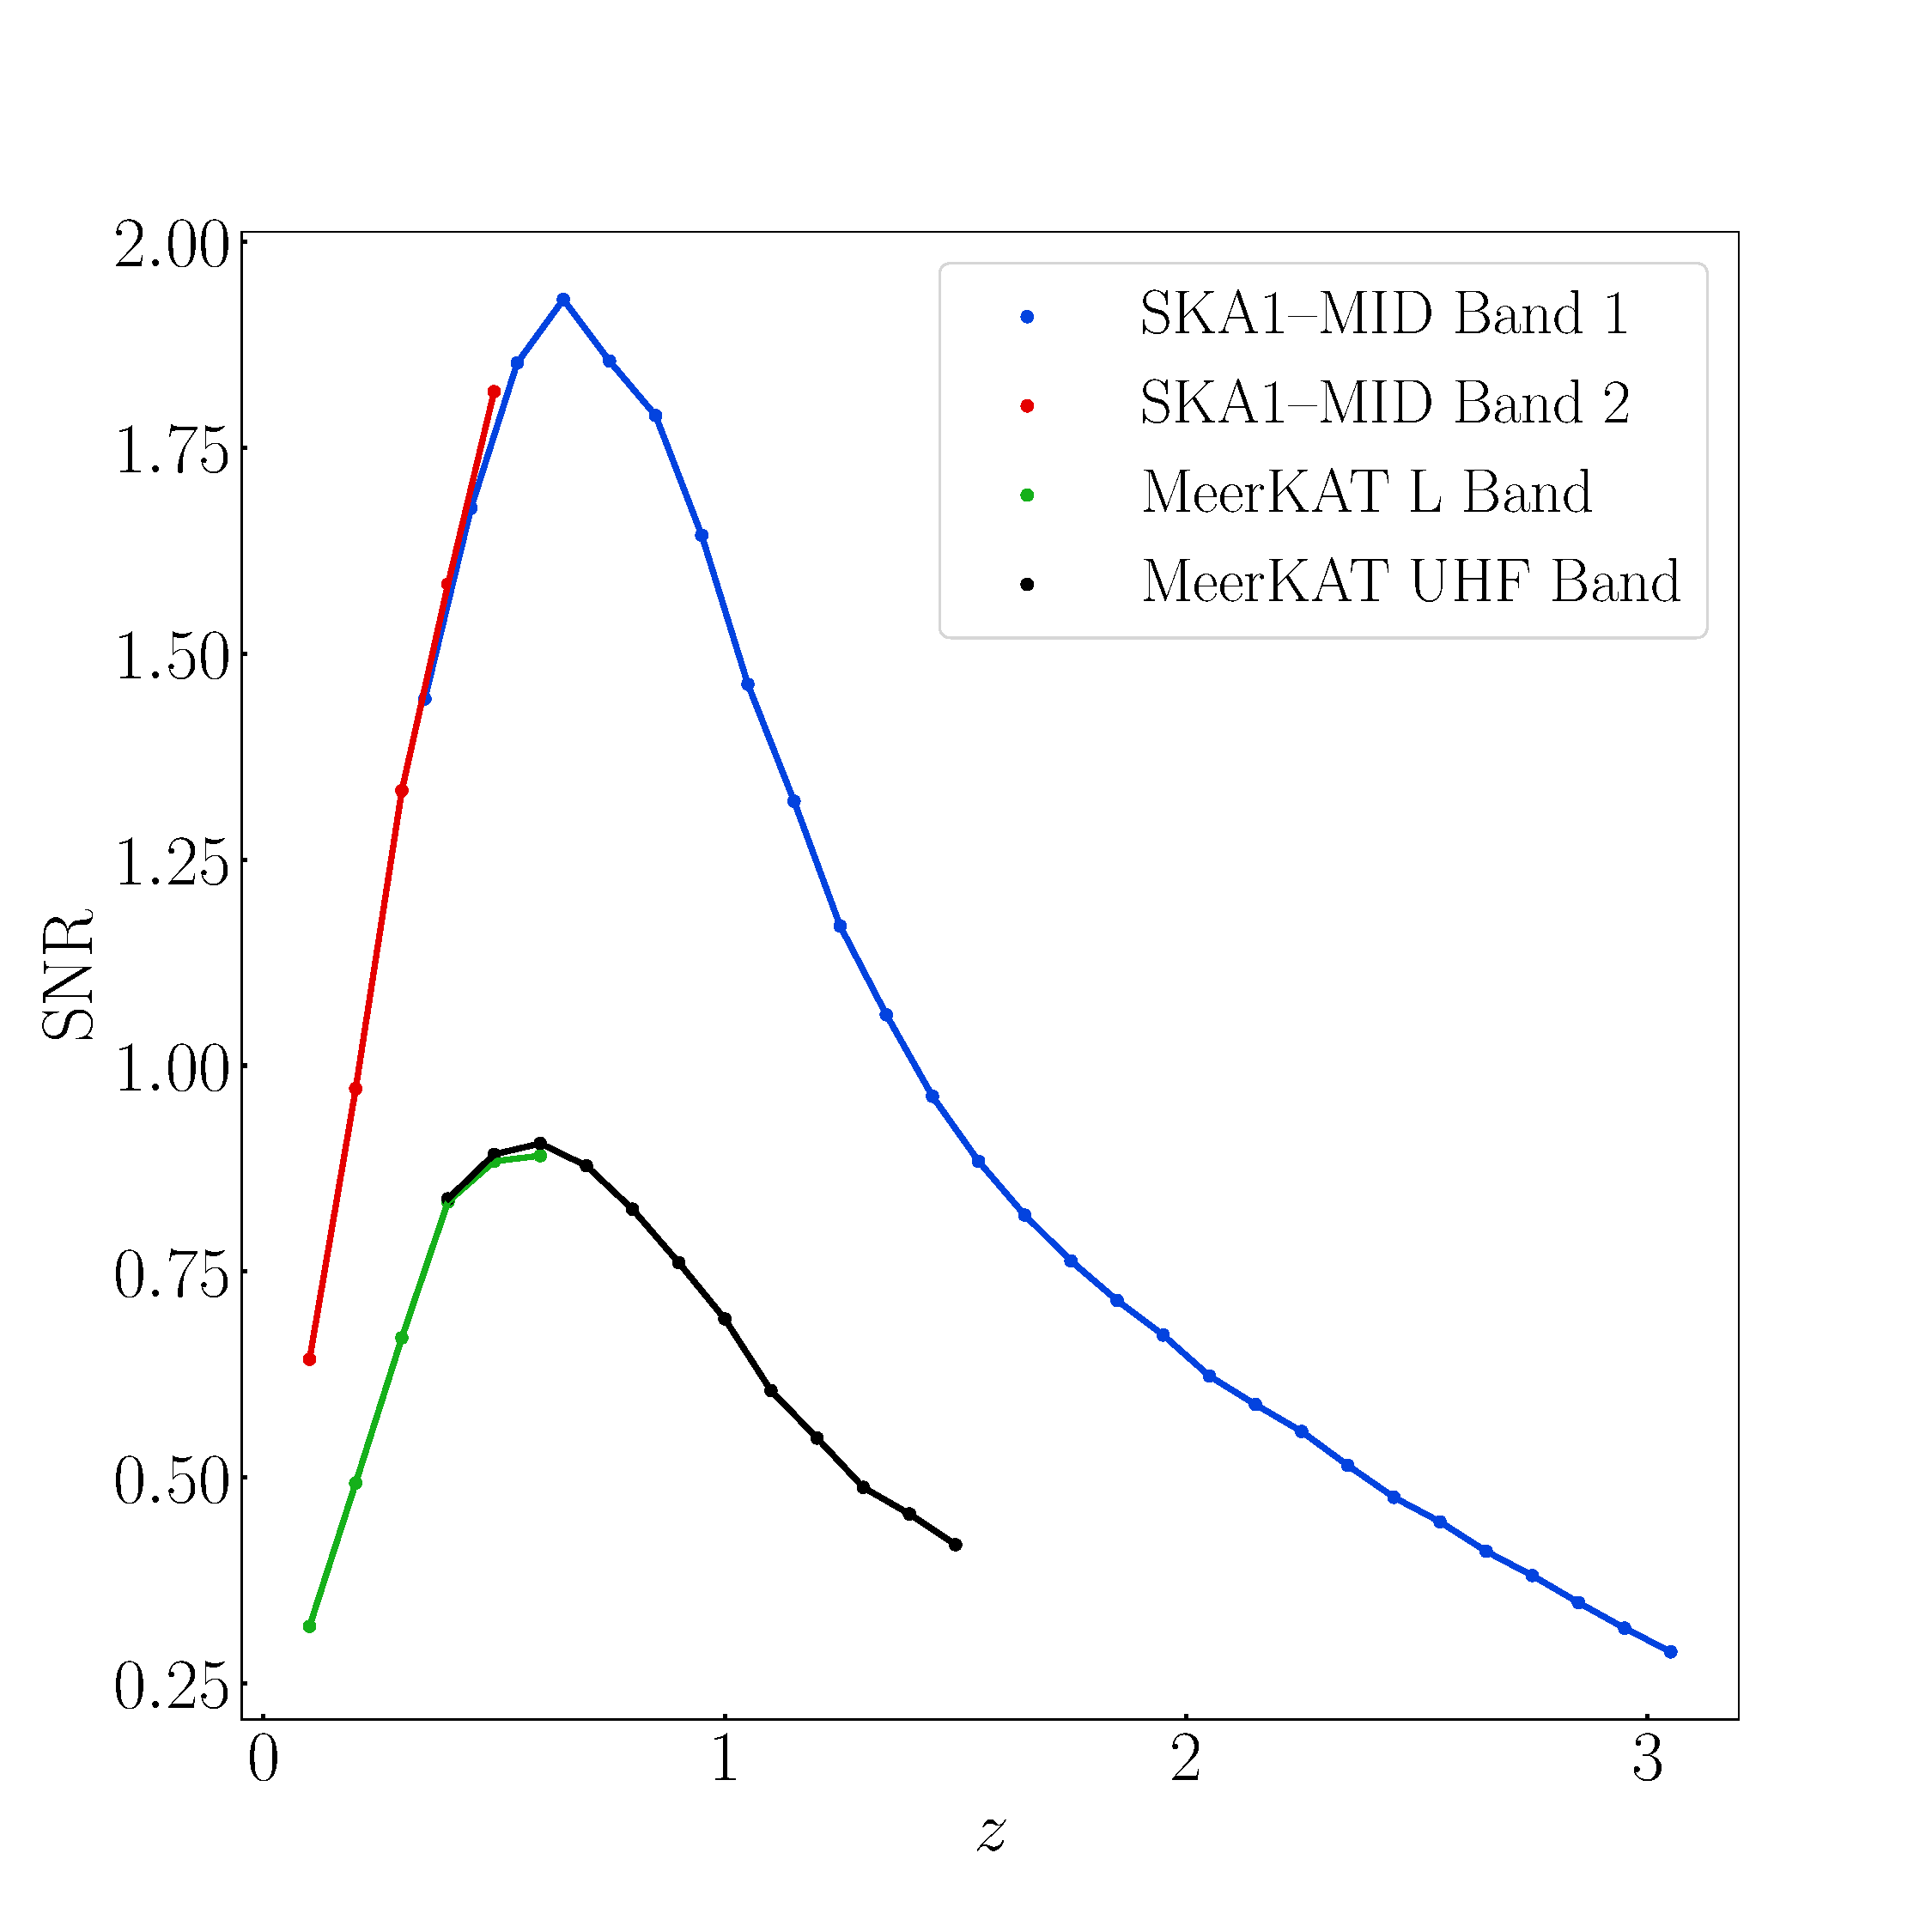
\includegraphics[width=.49\textwidth]{fig/snrSingleDishDopplerBg}
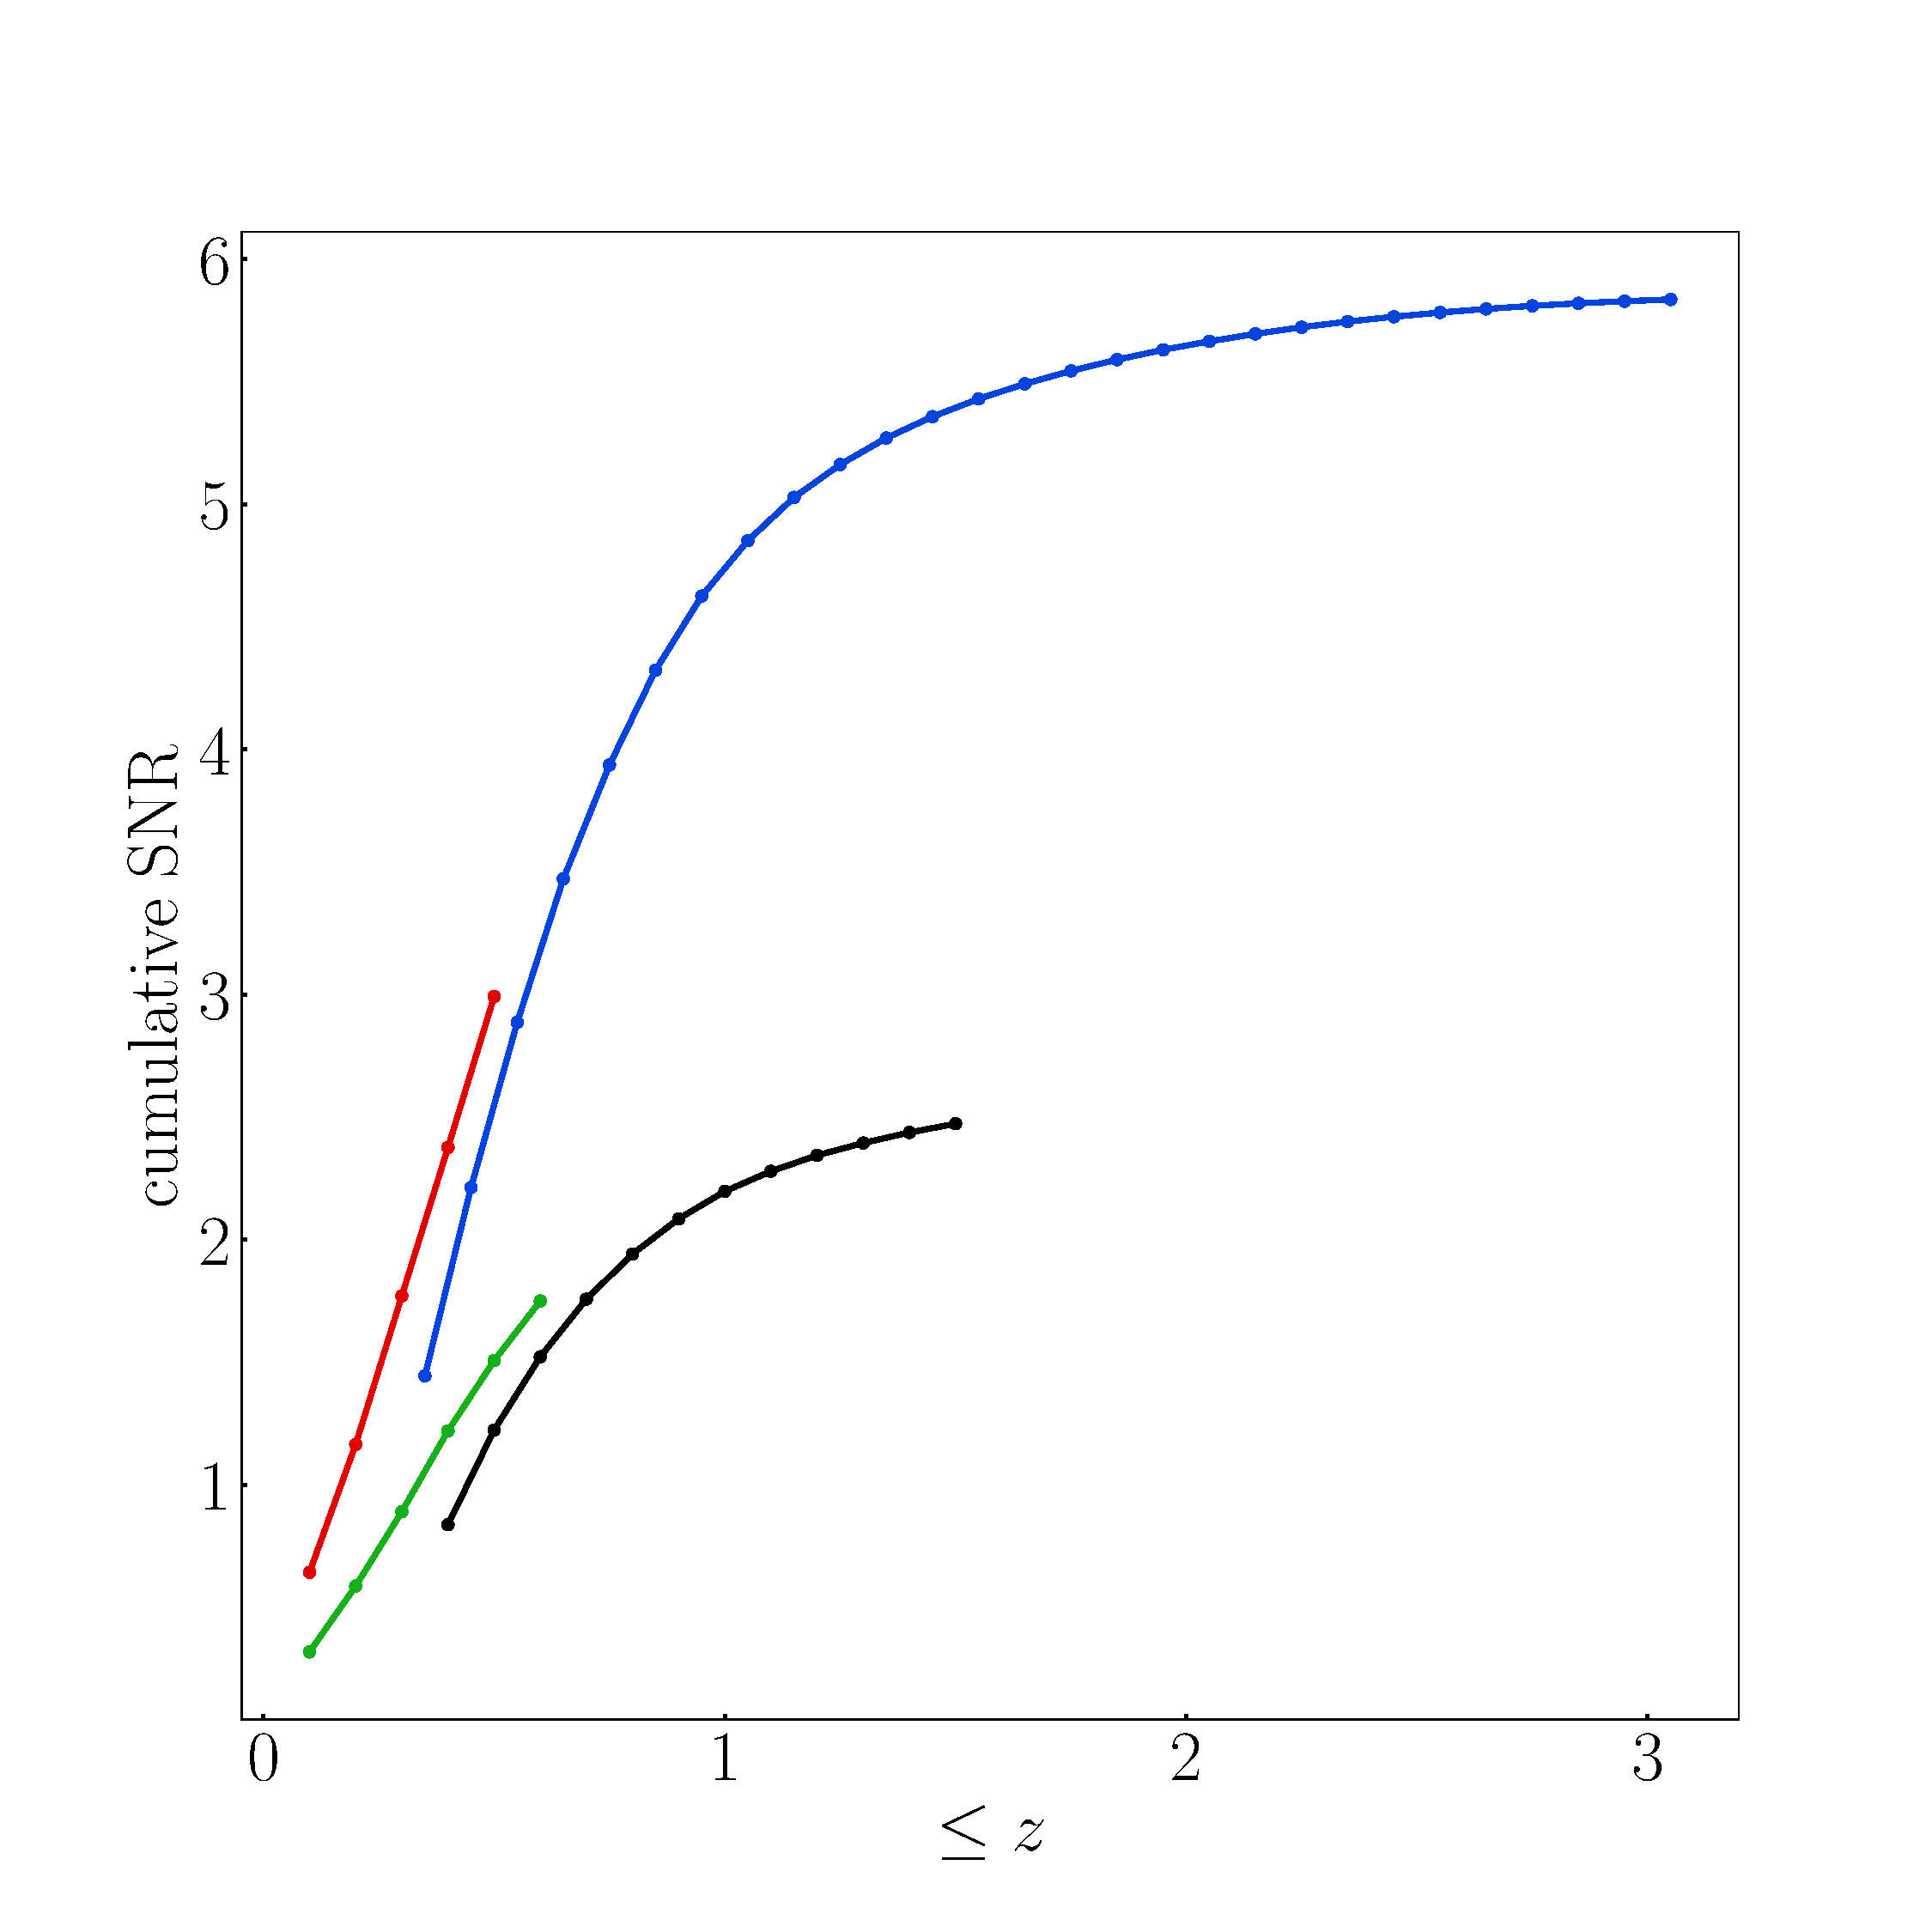
\includegraphics[width=.49\textwidth]{fig/snrSingleDishCumDopplerBg} 
\caption{SNR of the relativistic bispectrum per $z$-bin (\emph{left}) and cumulative (\emph{right}) for  SD-mode surveys. }
\label{fig3}
\end{figure}
\begin{table}[ht]
\centering
\caption{\label{tab3} Total SNR for single-dish mode surveys.} 
\vspace*{0.2cm}
\begin{tabular}{|lc|} \hline
Survey & Total SNR \\ \hline\hline 
MeerKAT UHF Band & 2.5 \\
MeerKAT L  Band & 1.8 \\
\hline
MeerKAT L+UHF Bands & {\bfseries 3.0}  \\
\hline
SKA1-MID Band 1 & 5.8 \\
SKA1-MID Band 2 & 3.0 \\
\hline
SKA1-MID Bands 1+2 & {\bfseries 6.6} \\
\hline
\end{tabular}
\end{table} 

The total SNR for the HI IM surveys in SD mode is {$3 \lesssim \mathrm{SNR} \lesssim 7$, with the high-$z_\mathrm{max}$ bands giving higher SNR.} 
Table~\ref{tab3} displays the predicted total SNR for the SD-mode HI IM surveys.
We can slightly improve the best total SNR by combining measurements in the two bands, for both MeerKAT and SKA.  In general, since we ignore cross-redshift correlations, we can sum in quadrature the per-bin values, $\mathrm{SNR}(z_i)$, as if they were a collection of bins from the same set of observations.
However, it must be noted that the two bands overlap in the redshift range  $0.40\leq z\leq 0.58$ for MeerKAT and $0.35\leq z \leq 0.49$ for SKA.
In that range, we follow a conservative approach and only consider the band yielding the largest value of SNR.
The values obtained are shown in Table~\ref{tab3}.

The best case, SKA1 Bands 1+2 gives a total SNR\, $\sim$6 that is detectable, a few times smaller than the SNR predicted for a Stage IV H$\alpha$ (similar to {\em Euclid}) spectroscopic survey~\cite{Maartens:2019yhx}. 
%
\subsubsection{Interferometer mode experiments}
%
\begin{figure}[ht!]
\centering
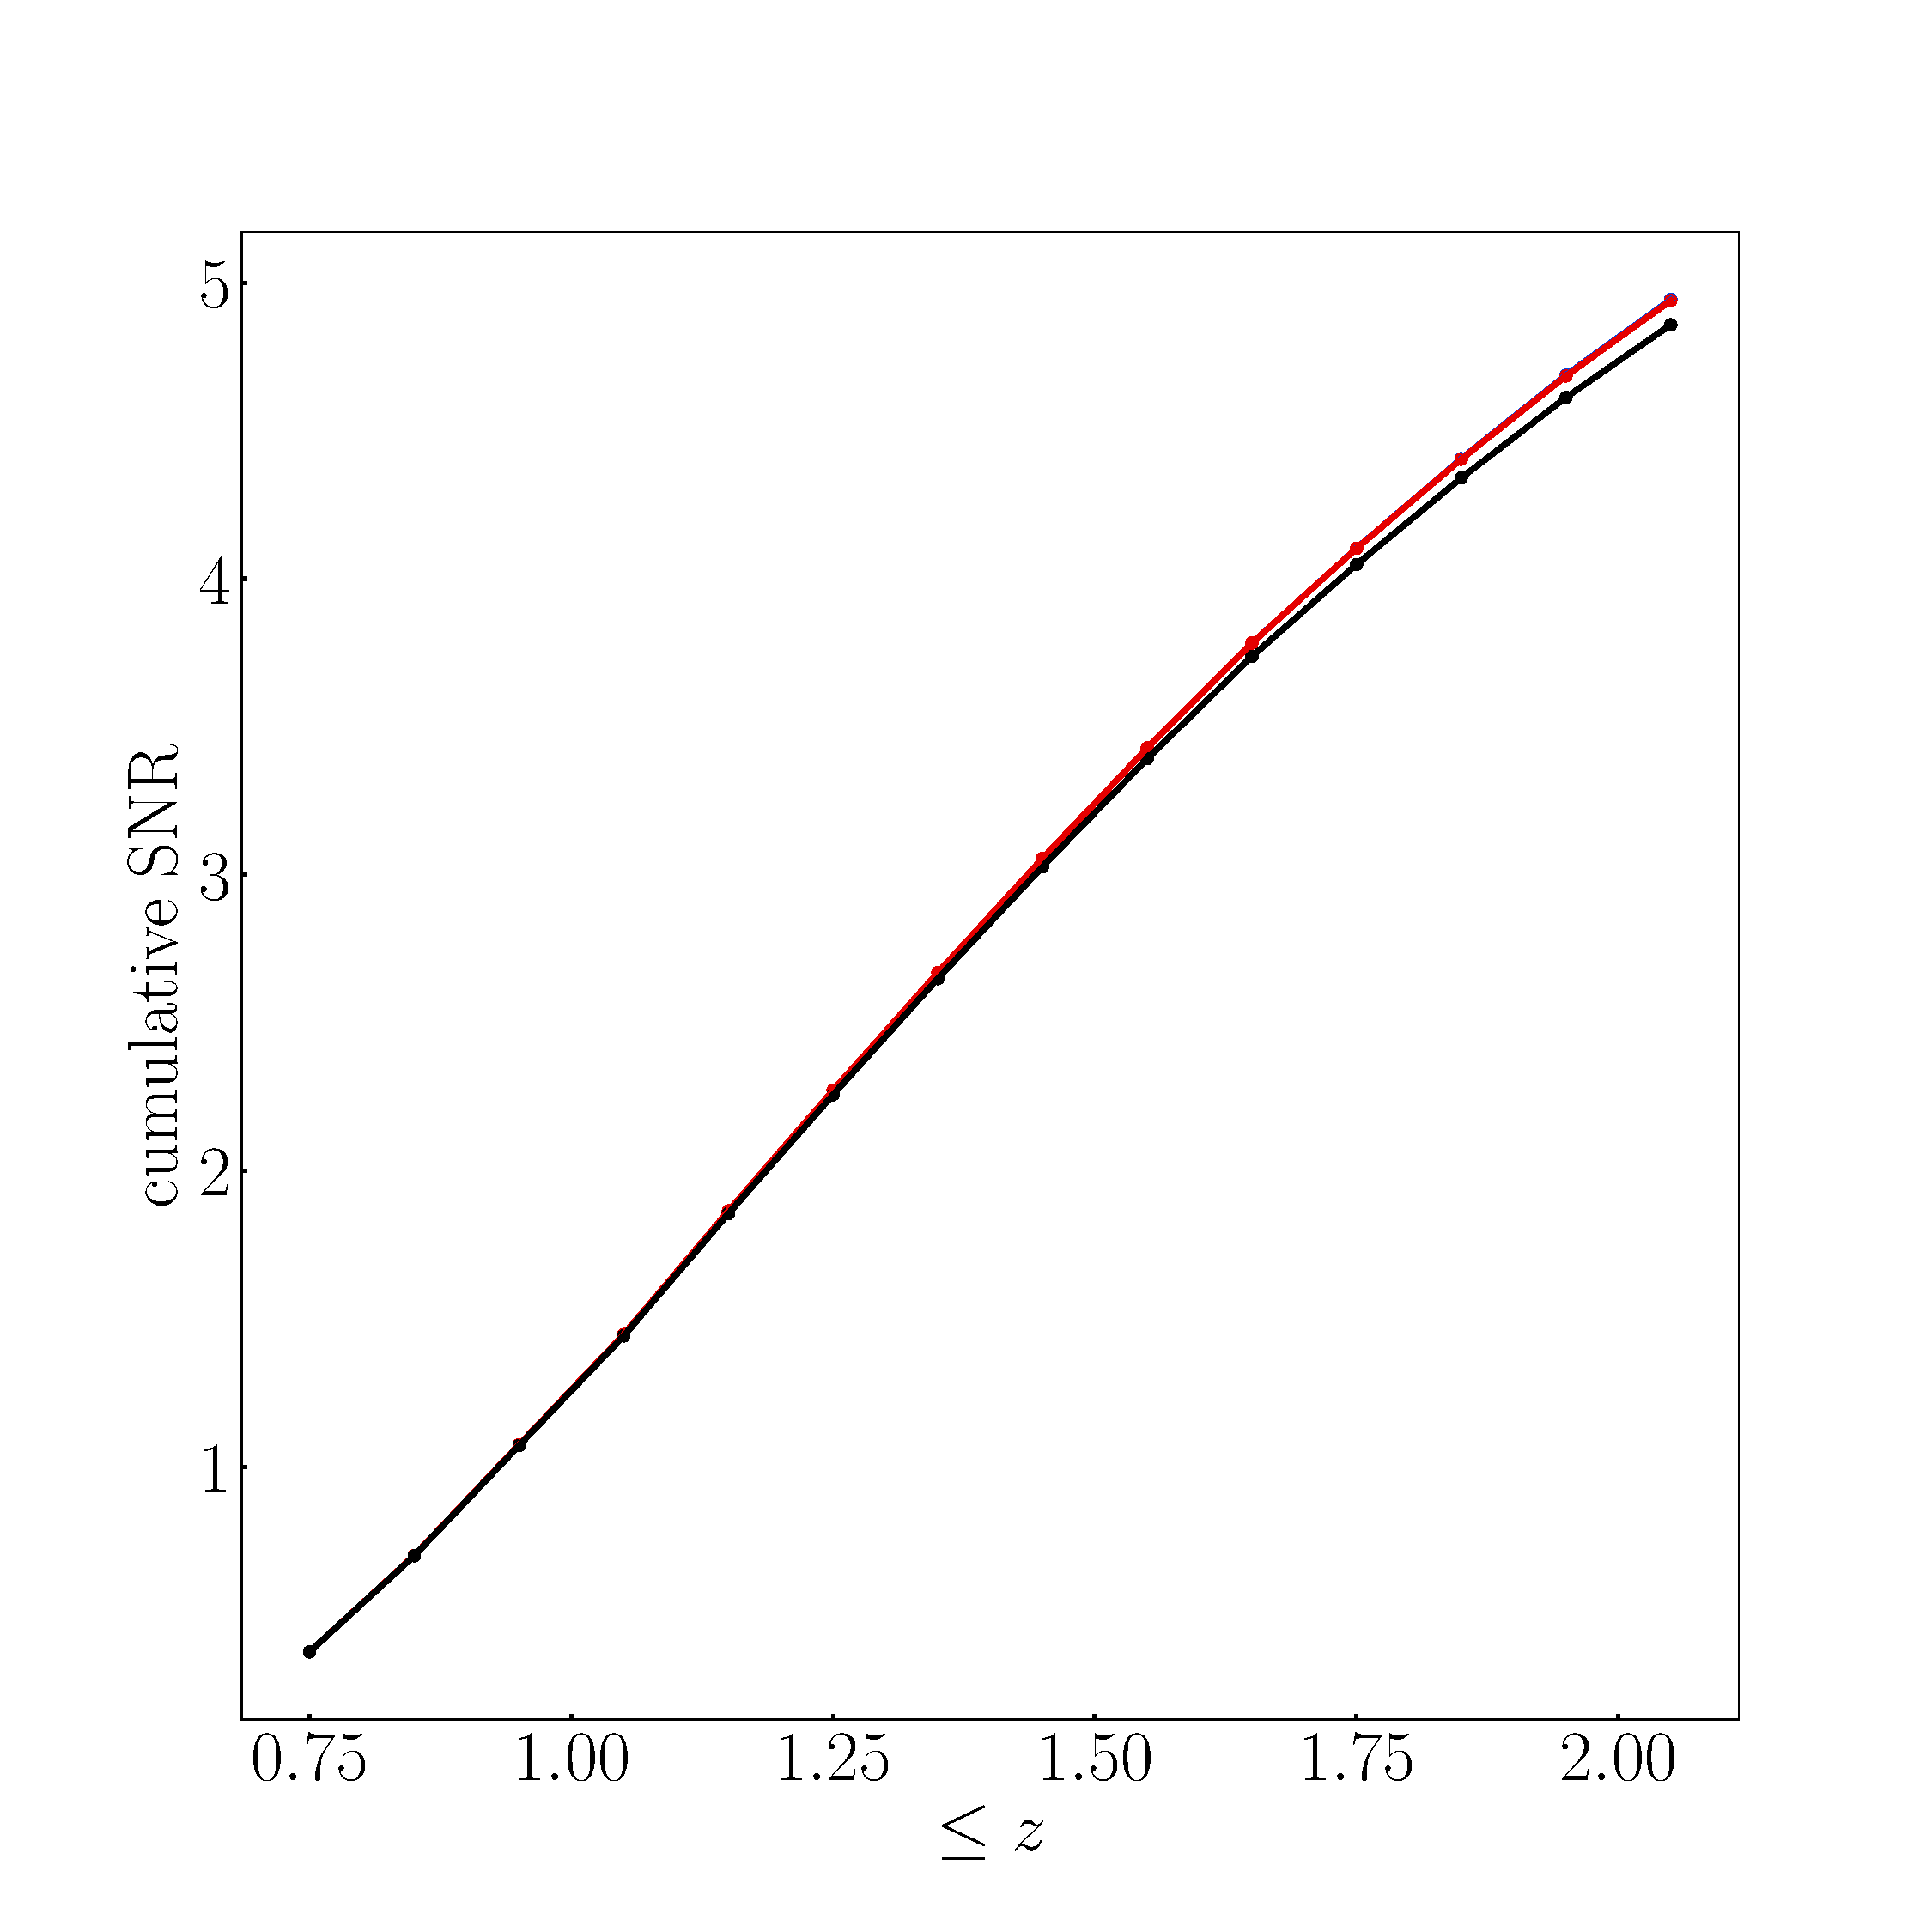
\includegraphics[width=.49\textwidth]{fig/snrInterferometerHIRAXCumDopplerBg}  
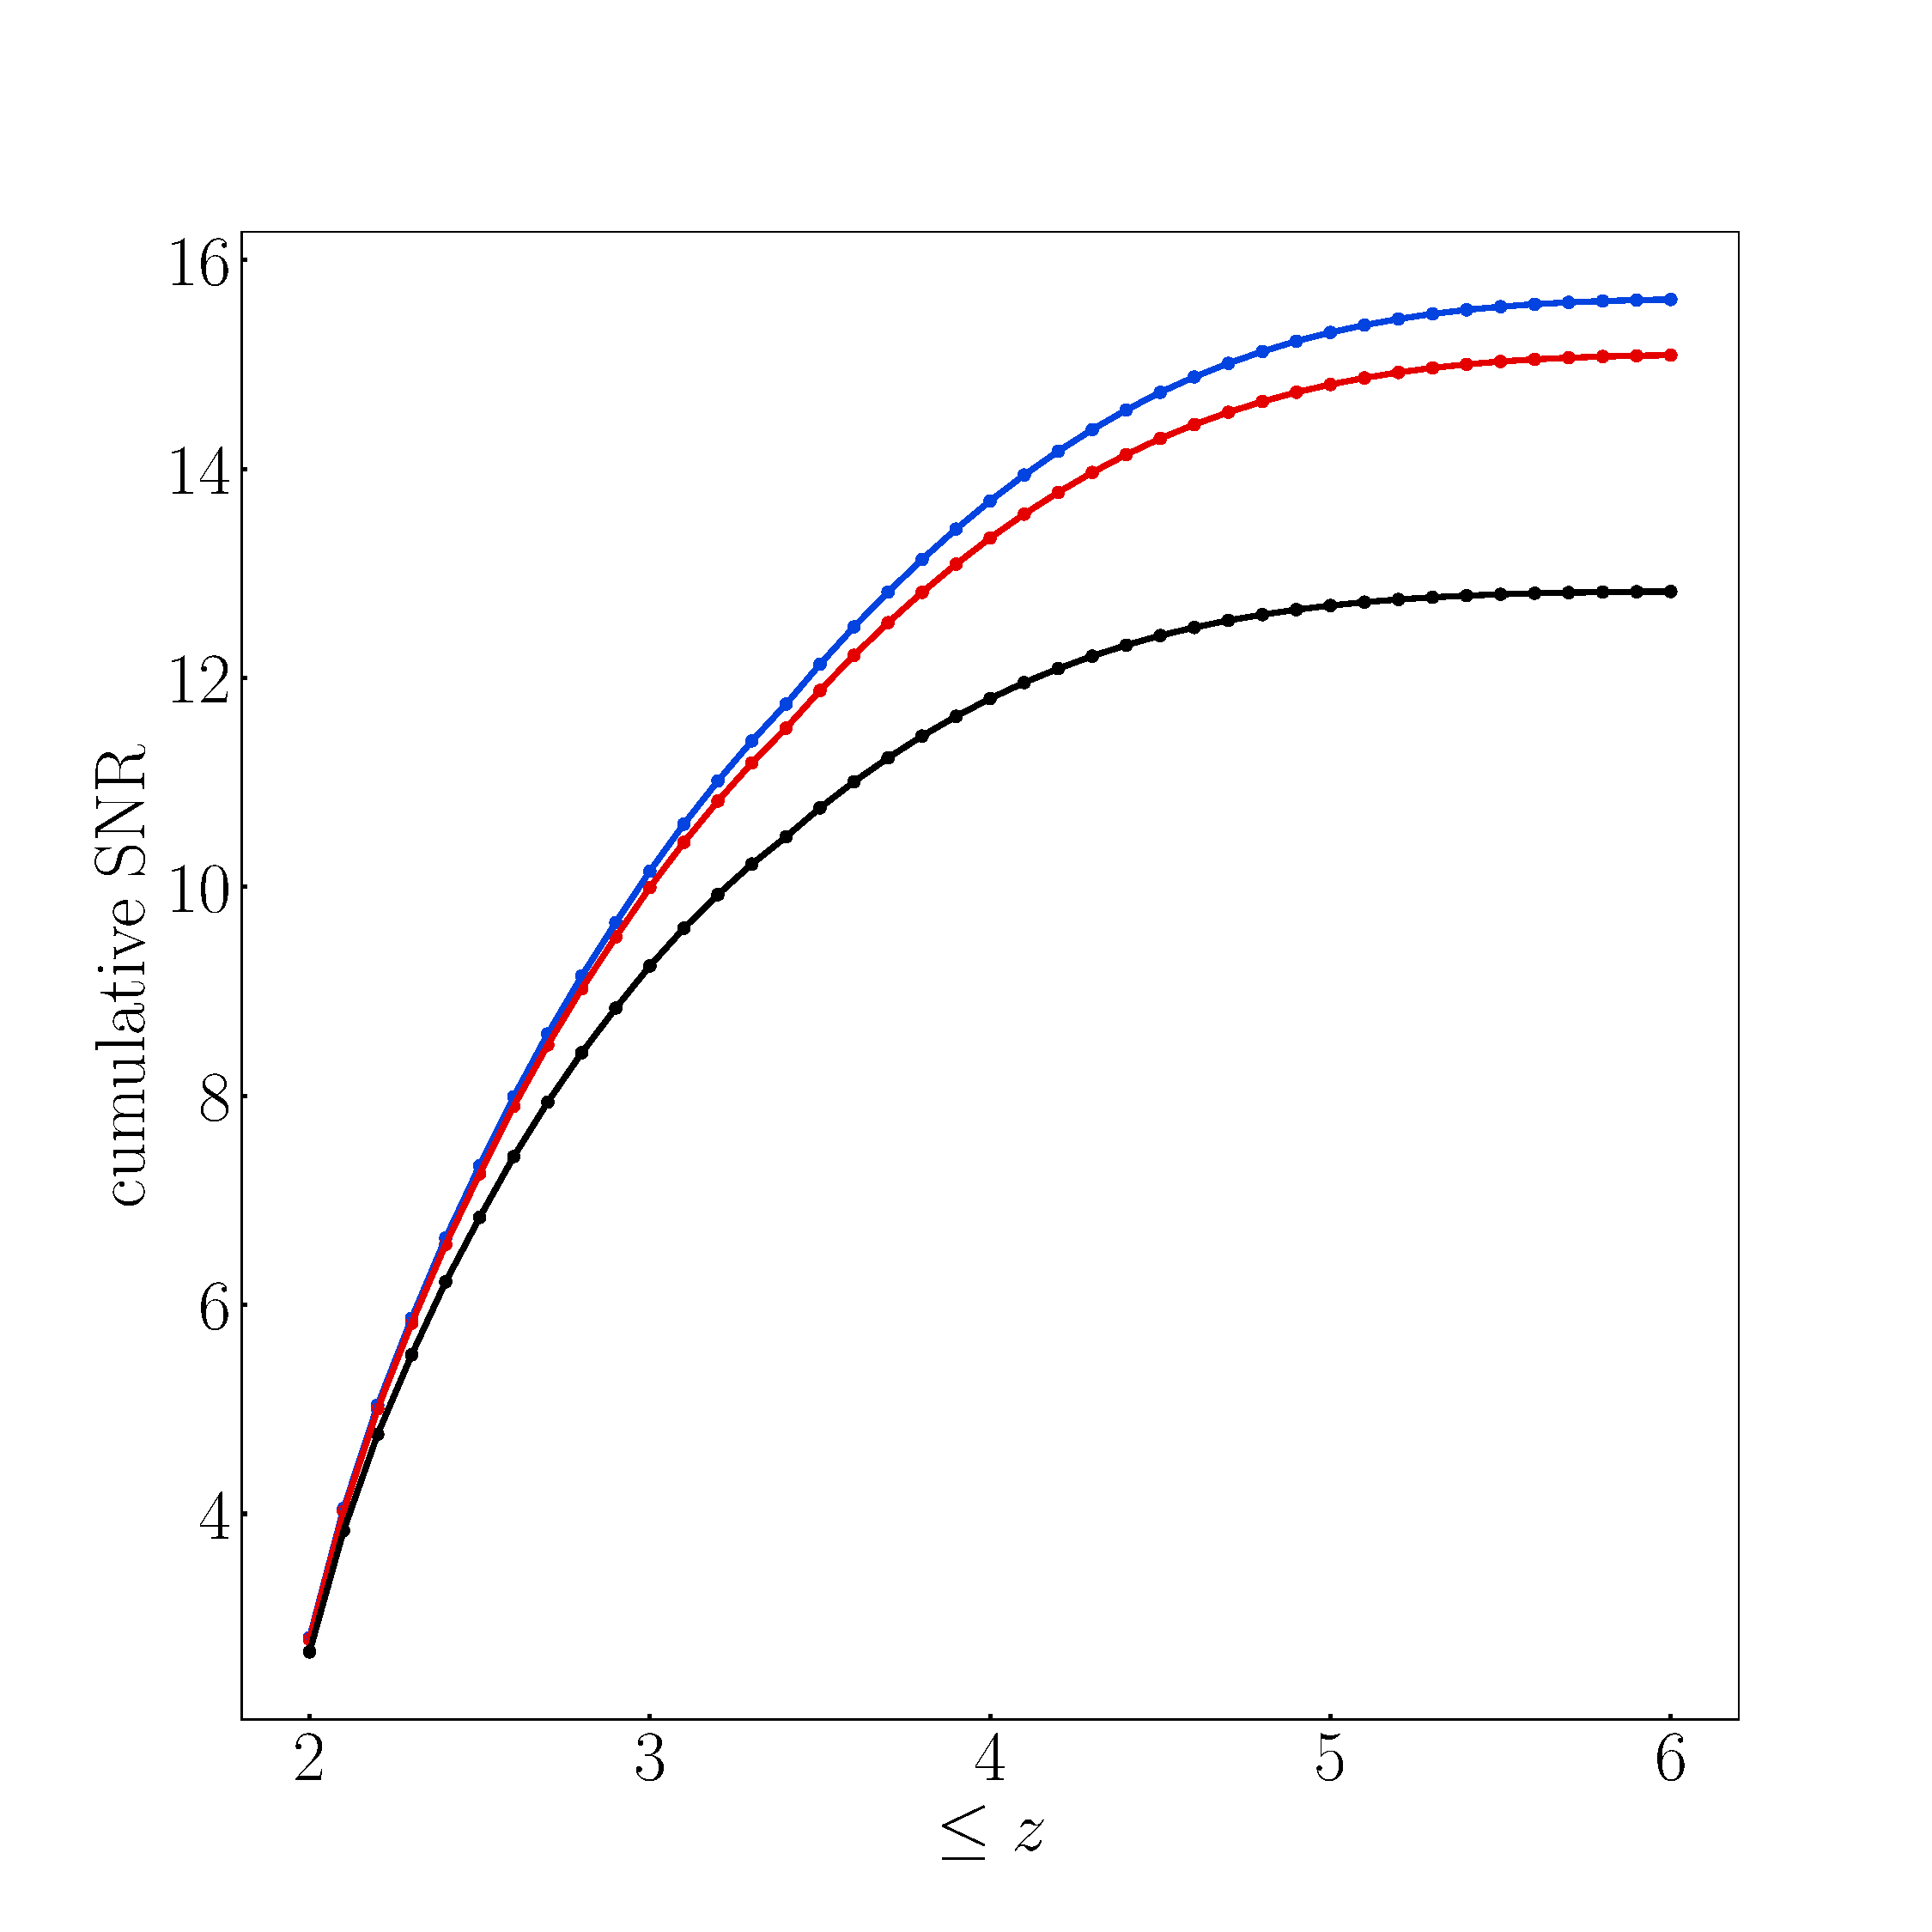
\includegraphics[width=.49\textwidth]{fig/snrInterferometerPUMAPetiteCumDopplerBg}
\caption{Cumulative SNR of the relativistic bispectrum for IF-mode surveys.}
\label{fig:imsnrres}
\end{figure}

\noindent Figure~\ref{fig:imsnrres} shows the forecasts of the relativistic bispectrum SNR for HIRAX and PUMA, using three values of the wedge parameter $N_\mathrm{w}$. 
HIRAX predicts SNR values slightly lower than an SKA SD-mode survey. The proposed PUMA survey (the `Petite' or PUMA--5K phase of the full or PUMA--32K proposal) gives the highest SNR, at a level similar to a Stage IV H$\alpha$ ({\em Euclid}-like) spectroscopic survey. This SNR would safely detect the relativistic signal.
Note that PUMA is more sensitive than HIRAX to the $N_\mathrm{w}$ parameter. 
Table~\ref{tab4} gives the predicted total SNR for the  IF-mode surveys.
\begin{table}[!ht]
\centering
\caption{\label{tab4} Total SNR for interferometer-mode surveys.} 
\vspace*{0.2cm}
\begin{tabular}{|l||*{5}{c|}}\hline
\backslashbox{Survey}{$N_{\mathrm{w}}$}
&\makebox[3em]{0}&\makebox[3em]{1}&\makebox[3em]{3} \\ \hline\hline
HIRAX &{5.4} & {\bfseries 5.4} & 5.3 \\ \hline
PUMA (Petite) & {14.5}& {\bfseries 14.0} & {12.0}\\ \hline
\end{tabular} 
\end{table}

\subsubsection{Reducing the radial foreground cut}
%
{We investigate how much improvement in SNR results if we increase the number of very large scale modes by reducing the radial foreground cut to $k_{\parallel\mathrm{fg}}=0.005\,h\mathrm{Mpc}^{-1}$. Such a reduction may be achieved by future advances in reconstruction techniques. 

It turns out that the SNR is relatively insensitive to this reduction in $k_{\parallel\mathrm{fg}}$: very little gain in SNR is achieved, as shown in Tables~\ref{tab5a} and~\ref{tab6}.}

\begin{table}[!ht]
\centering
\caption{\label{tab5a} Total SNR for single-dish mode surveys with $k_{\parallel\mathrm{fg}}=0.005\,h\mathrm{Mpc}^{-1}$. }
\vspace*{0.2cm}
\begin{tabular}{|lc|} \hline
Survey & Total SNR \\ \hline\hline 
MeerKAT UHF Band & 2.8  \\
MeerKAT L Band & 2.0  \\
\hline
MeerKAT L+UHF Bands & {\bfseries 3.4}  \\
\hline
SKA1-MID Band 1 & 6.5 \\
SKA1-MID Band 2 & 3.4 \\
\hline
SKA1-MID Bands 1+2 & {\bfseries 7.3} \\
\hline
\end{tabular}
\end{table} 
\begin{table}[!ht]
\centering
\caption{\label{tab6} Total SNR for interferometer-mode surveys with $k_{\parallel\mathrm{fg}}=0.005\, h\mathrm{Mpc}^{-1}$.} 
\vspace*{0.2cm}
\begin{tabular}{|l||*{5}{c|}}\hline
\backslashbox{Survey}{$N_{\mathrm{w}}$}
&\makebox[3em]{0}&\makebox[3em]{1}&\makebox[3em]{3} \\ \hline\hline
HIRAX & 5.6 & {\bfseries 5.6} & 5.5 \\ \hline
PUMA (Petite) & 15.2 & {\bfseries 14.6} & 12.5 \\ \hline
\end{tabular} 
\end{table}
%
%
\section{Conclusions} \label{sec5}
%
%
The imaginary part of the galaxy bispectrum at leading order is a unique signal that is purely relativistic~\cite{Clarkson:2018dwn} -- and that can be readily extracted from the full bispectrum. In Fourier space, the leading-order local lightcone effects that generate the Doppler-type signal scale as $\i\left(\cH/k\right)$ (see~\eqref{e1.9} and~\eqref{e1.10}). In the galaxy power spectrum for a single tracer, these Doppler-type contributions only occur squared, thus scaling as $\cH^2/k^{2}$. Only a cross-power spectrum analysis of two different tracers will generate an imaginary contribution~\cite{McDonald:2009dh}. For single tracers, the relativistic Doppler-type signal in the power spectrum is therefore highly suppressed and not detectable, even for a cosmic-variance limited survey~\cite{Alonso:2015uua}.

However, in the bispectrum of a single tracer, the $\i \left(\cH/k\right)$ relativistic signal survives because it couples with the Newtonian terms~\cite{Clarkson:2018dwn}. This increases the chance of detectability and, as shown by~\cite{Maartens:2019yhx}, the SNR forecast for a Stage IV H$\alpha$ galaxy spectroscopic survey  (similar to {\em Euclid}) is $\sim$17. 

We extended the analysis of~\cite{Maartens:2019yhx} to HI intensity mapping spectroscopic surveys, which requires significant additions in order to deal with foreground contamination and the complexities of instrumental noise (that dominates over shot noise). As expected, loss of signal due to foreground cleaning and telescope beam effects reduces the SNR for the next-generation surveys on MeerKAT, SKA1-MID and HIRAX. 
We forecast a detectable SNR\,$\sim$6 for SKA1 and $\sim$5 for HIRAX.
The proposed PUMA survey in its Petite or 5,000-dish first phase (before the futuristic full survey with 32,000 dishes) delivers a SNR $\sim$14, comparable to that  of a Stage IV H$\alpha$ galaxy survey.

Surveys in single-dish mode (MeerKAT, SKA1) suffer from poor angular resolution so that the Newtonian short-scale transverse modes are suppressed.  On the other hand, the interferometer-mode surveys (HIRAX, PUMA) do not probe ultra-large scales as well as SD-mode surveys because the maximum length scale is determined  by the minimum baseline~\eqref{kifmin}, as shown in Figure~\ref{pnoise}.

We investigated the effect of a more optimistic radial wavenumber cut and found that the improvement in SNR is small. This means that detection of the relativistic signal in the bispectrum does not require scales with $k\lesssim 0.01h/$Mpc. 

There are some caveats to our results and pointers for future work: 
\begin{itemize}
\item
In common with nearly all work on the Fourier-space bispectrum that includes RSD, we implicitly make a flat-sky assumption, based on the fixed global direction $\n$. This is an issue when probing ultra-large scales -- which applies not only to our case but also to all work on constraining primordial non-Gaussianity via the Fourier bispectrum. 
The flat-sky analysis loses accuracy as $\theta$ increases, where $\theta$ is the maximum opening angle to the three-point correlations at the given redshift. The corresponding comoving transverse scale is $k_\perp(z) = 2\pi/\left[r(z) \theta\right]$. There is a threshold scale  
$\theta_\mathrm{fs}$, beyond which the  approximation fails -- i.e., for $\theta> \theta_\mathrm{fs}$, or equivalently, $k_\perp < k_{\perp \mathrm{fs}}$, the SNR is not reliable.

For IF-mode surveys, the flat-sky assumption is reasonable if $\theta_\mathrm{fs}> \theta_\mathrm{b}$, where $\theta_\mathrm{b}$ is the beam, given by \eqref{thetab}. If we estimate that $\theta_\mathrm{fs} \sim 10^\circ$ (see~\cite{Matsubara:1999du}), then this condition holds for HIRAX, and for PUMA up to redshift 3 (see Figure~\ref{figmin}).
Consequently, the flat-sky assumption is reasonable for HIRAX. However for PUMA at $z>3$ and for the SD-mode surveys, there are modes with $k_\perp < k_{\perp \mathrm{fs}}$ and the accuracy of the SNR will be affected for these modes.

Including wide-angle effects is a key target for future work that constrains relativistic effects or primordial non-Gaussianity via the bispectrum. In fact, this is also important for standard cosmological constraints.
Corrections to the global flat-sky analysis of the Fourier bispectrum can be made by using a local flat-sky approximation~\cite{Scoccimarro:2015bla,Sugiyama:2018yzo}.
Such corrections are typically approximate and do not incorporate the full wide-angle effect. Ultimately, one needs to use the full-sky 3-point correlation function or the full-sky angular bispectrum (see e.g.~\cite{Kehagias:2015tda, DiDio:2016gpd, DiDio:2018unb, Durrer:2020orn}) to properly include all wide-angle correlations. These alternatives are computationally much more intensive than the Fourier analysis.

\item 
Also in common with other work on the Fourier power spectrum and bispectrum, we neglect cross-correlations among redshift bins.  This is justified by the exquisite redshift accuracy of HI intensity mapping, allowing for sharp-edged redshift bins, which in turn implies small or no overlap between them. Integrated effects will in principle induce correlations along the line-of-sight direction, but this is not going to be relevant in our case since the dominant integrated contribution is weak lensing magnification, which vanishes in HI intensity mapping~\cite{Hall:2012wd,Alonso:2015uua,DiDio:2015bua,Jalivand:2018vfz}.    
Ultimately, only approximate solutions are possible in Fourier space and a complete treatment would require the angular bispectrum or 3-point correlation function.
\item 
In the absence of a simulation-based model for the bispectrum RSD damping parameter $\sigma_B$, we set it equal to the power spectrum damping parameter $\sigma_P$, for which we used a fit from simulations given in~\cite{Sarkar:2019nak}. Realistically, we expect that $\sigma_B >\sigma_P$. We tested the impact  on the SNR of increasing $\sigma_B$ to $\sigma_B=1.5\, \sigma_P$ and found that it leads to only a small decrease in SNR. 

\end{itemize}



